\immediate\write18{makeindex Index.nlo -s nomencl.ist -o Index.nls}
%%%%%%%%%%%%%%%%%%%%%%%%%%%%%%%%%%%%%%%%%%%%%%%%%%%%%%%%%%%%%%%%%%%%%%%%
%%                                                                    %%
%% This is file `ucalgarythesis.tex'  -- a document template for      %%
%% graduate theses at the University of Calgary.                      %%
%%                                                                    %%
%% This template document is to be used in conjunction with the       %%
%% thesis class file `ucalgarythesis.cls'.                            %%
%%                                                                    %%
%% Created by M.W. Girard, last updated 10 April 2016.                %%
%%                                                                    %%
%% This template was created to be in compliance with the University  %%
%% of Calgary thesis guidelines (version 14 April 2014)               %%
%%       https://grad.ucalgary.ca/current/thesis/guidelines.          %%
%%                                                                    %%
%%%%%%%%%%%%%%%%%%%%%%%%%%%%%%%%%%%%%%%%%%%%%%%%%%%%%%%%%%%%%%%%%%%%%%%%
%%                                                                    %%
%% By default, the text of the thesis is double spaced and should be  %%
%% printed single-sided. All margins must be exactly one inch on all  %%
%% sides, and should not be bound or have binding edges. This is      %%
%% required by the University of Calgary thesis guidelines.           %%
%% All theses are now required to be submitted electronically.        %%
%%                                                                    %%
%%%%%%%%%%%%%%%%%%%%%%%%%%%%%%%%%%%%%%%%%%%%%%%%%%%%%%%%%%%%%%%%%%%%%%%%


%%%%%%%%%%%%%%%%%%%%%%%%%%%%%%%%%%%%%%%%%%%%%%%%%%%%%%%%%%%%
%%
%% Load the `ucalgarythesis.cls' document class
%%%%%%%%%%%%%%%%%%%%%%%%%%%%%%%%%%%%%%%%%%%%%%%%%%%%%%%%%%%%

  \documentclass{ucalgarythesis}
  
  %%%%%%%%%%%%%%%%%%%%%%%%%%%%%%%%%%%%%%%%%%%%%%%%%%%%%%%%%%%%%%%%%%%%%%
  %% If you would like to print a personal copy of your thesis for    %%
  %% your own record, you may print it double-sided and with extra    %%
  %% margins for binding. Use the following line instead of the above %%
  %% \documentclass{ucalgarythesis} for compiling personal copies of  %%
  %% the thesis to be printed double-sided and bound.                 %%
  %%%%%%%%%%%%%%%%%%%%%%%%%%%%%%%%%%%%%%%%%%%%%%%%%%%%%%%%%%%%%%%%%%%%%%
  %\documentclass[twoside,binding]{ucalgarythesis}

%%%%%%%%%%%%%%%%%%%%%%%%%%%%%%%%%%%%%%%%%%%%%%%%%%%%%%%%%%%%
%%
%% Imported packages & custom user commands
%%%%%%%%%%%%%%%%%%%%%%%%%%%%%%%%%%%%%%%%%%%%%%%%%%%%%%%%%%%%

%% Include extra packages here

\usepackage{float} % for figure fix H

\usepackage[utf8]{inputenc}
\usepackage{amssymb,amsthm,amsmath}
\usepackage[hidelinks]{hyperref}
  
\usepackage{graphicx}
\DeclareGraphicsExtensions{.pdf,.png}

\usepackage[numbers,sort]{natbib} % for bibliography

\usepackage{amsmath,amssymb,amsfonts}
\usepackage{algorithm}
% \usepackage{algorithmicx}
\usepackage{algpseudocode}

\usepackage{textcomp}
\usepackage{xcolor}
\usepackage{caption}
\usepackage{listings}

\usepackage{url} 	% for URLs with hyperlink use: hyperref
\newcommand{\squeezeup}{\vspace{-30mm}}	% to reduce space between figures and text
\usepackage{multirow}	% multi r/c of tables
\usepackage[euler]{textgreek}
%%  Include other user-defined commands here

\usepackage{booktabs}
\usepackage[parfill]{parskip}

%% Abbreviations
% \usepackage{nomencl}
\usepackage[intoc, english]{nomencl}
\makenomenclature

\usepackage{enumitem}	% for item spacing

\usepackage{pdflscape} % change landscape/ portrait mode

% Keep figures within their own subsection
\usepackage[section]{placeins}
\usepackage{subcaption} 

% For strike out
\usepackage{soul}
\newcommand{\prune}[1]{\textcolor{red}{\st{#1}}}

\usepackage{etoolbox}

  \theoremstyle{plain}
  \newtheorem{theorem}{Theorem}[chapter]
  \newtheorem{lemma}[theorem]{Lemma}
  \newtheorem{corollary}[theorem]{Corollary}
  
  \theoremstyle{definition}
  \newtheorem{definition}[theorem]{Definition}

\definecolor{red}{RGB}{205, 92, 92}
\newcommand{\todo}[1]{\hfill \break [\textcolor{red}{\textbf{TODO:}} #1]}
% \newcommand{\todo}[1]{\hfill \break [\textcolor{red}{\textbf{TODO:}} #1]\PackageWarning{TODO:}{#1}}
% \newcommand{\todo}[1]{\hfill \break - #1}

\newcommand{\content}[1]{#1}
% \newcommand{\content}[1]{\space}


\newcommand*{\figuretitle}[1]{
    {\centering
    \textbf{#1}
    \par\medskip}
}

%% ABBREVIATIONS

\newcommand{\Name}[0]{\underline{Ru}le set \underline{G}eneration \underline{R}epeated on \underline{A}ltering \underline{T}ime \underline{S}cales }
\newcommand{\Abb}[0]{RuGRATS }
\newcommand{\RIPPER}[0]{\underline{R}epeated \underline{I}ncremental \underline{P}runing to \underline{P}roduce \underline{E}rror \underline{R}eduction }
\newcommand{\IREP}[0]{\underline{I}ncremental \underline{R}educed \underline{E}rror \underline{P}runing }
\newcommand{\FOIL}[0]{\underline{F}irst-\underline{O}rder \underline{I}nductive \underline{L}earner}


%%%%%%%%%%%%%%%%%%%%%%%%%%%%%%%%%%%%%%%%%%%%%%%%%%%%%%%%%%%%%%%%%%%%%%%%
%%                                                                    %%
%% Begin document                                                     %%
%%                                                                    %%
%%%%%%%%%%%%%%%%%%%%%%%%%%%%%%%%%%%%%%%%%%%%%%%%%%%%%%%%%%%%%%%%%%%%%%%%
\begin{document}

%%%%%%%%%%%%%%%%%%%%%%%%%%%%%%%%%%%%%%%%%%%%%%%%%%%%%%%%%%%%%%%%%%%%%%%%
%%                                                                    %%
%% Title page                                                         %%
%%                                                                    %%
%%%%%%%%%%%%%%%%%%%%%%%%%%%%%%%%%%%%%%%%%%%%%%%%%%%%%%%%%%%%%%%%%%%%%%%%

%%%%%%%%%%%%%%%%%%%%%%%%%%%%%%%%%%%%%%%%%%%%%%%%%%%%%%%%%%%%%%%%%%%%%%%%
%% Instructions for title page information:                           %%
%%                                                                    %%
%%  Fill in the following fields with the required information:       %%
%%   - \title{...}        Title of the thesis                         %%
%%   - \author{...}       Your full name                              %%
%%   - \thesis{Thesis}    Type of document (may change to `Thesis' to %%
%%                           `Dissertation' depending on type of work)%%
%%   - \dept{...}         Full name of the graduate department or     %%
%%                           degree program                           %%
%%   - \degree{...}       Full name of the degree obtained            %%
%%                          (i.e. Doctor of Philosophy,               %%
%%                                 Master of Science, etc)            %%
%%   - \gradyear{...}     Year of submission                          %%
%%   - \monthname{...}    Month of submission                         %%
%%%%%%%%%%%%%%%%%%%%%%%%%%%%%%%%%%%%%%%%%%%%%%%%%%%%%%%%%%%%%%%%%%%%%%%%

  \title{
  Design and Implementation of a Recommender System \\for use at an Emergency Homeless Shelter in Calgary
  % \\ \bigskip
	% [The \Abb system]
   }
   
  \author{Caleb Thomas John}
  \thesis{Thesis}
  \dept{Graduate Program in Electrical Engineering}
  \degree{Master of Science}
  \gradyear{2021}
  \monthname{April}
  

%%%%%%%%%%%%%%%%%%%%%%%%%%%%%%%%%%%%%%%%%%%%%%%%%%%  
%% Make the thesis title page.
%%%%%%%%%%%%%%%%%%%%%%%%%%%%%%%%%%%%%%%%%%%%%%%%%%%
  \frontmatter           %% Don't remove this line.
  \makethesistitle       %% Don't remove this line.


%%%%%%%%%%%%%%%%%%%%%%%%%%%%%%%%%%%%%%%%%%%%%%%%%%%%%%%%%%%%%%%%%%%%%%%%
%%                                                                    %%
%% Prefatory pages                                                    %%
%%                                                                    %%
%%%%%%%%%%%%%%%%%%%%%%%%%%%%%%%%%%%%%%%%%%%%%%%%%%%%%%%%%%%%%%%%%%%%%%%%
%% The following sections are in the correct order as specified by    %%
%% April 2014 thesis guidelines set by the University of Calgary. %%
%%                                                                    %%
%% You may remove optional sections, but do not change the order.     %%
%%%%%%%%%%%%%%%%%%%%%%%%%%%%%%%%%%%%%%%%%%%%%%%%%%%%%%%%%%%%%%%%%%%%%%%%

%%%%%%%%%%%%%%%%%%%%%%%%%%%%%%%%%%%%%%%%%%%%%%%%%%%
%%
%% Abstract page (REQUIRED)
%%%%%%%%%%%%%%%%%%%%%%%%%%%%%%%%%%%%%%%%%%%%%%%%%%%

  \begin{thesisabstract}  
    Modern homeless shelters are collecting data from key interactions with clients. This data can be utilized by machine learning algorithms to identify clients that are at risk for chronic homelessness. This would provide shelter operators with a powerful new tool to assist them in housing individuals. However, most machine learning algorithms are not suitable for the task due to the lack of interpretability. Classification rule learning is brought forward in this work as an exceedingly interpretable class of machine learning algorithms.
A novel recommender system based on classification rule learning is proposed and evaluated on local homeless shelter data. The results from this work suggest that classification rule learning is robust and interpretable enough to be used to support modern homeless shelters.
		% A novel system based on classification rule learning was proposed and evaluated on local homeless shelter data. These results suggest that classification rule learning is robust enough to be considered for use in modern homeless shelters.
  \end{thesisabstract}


%%%%%%%%%%%%%%%%%%%%%%%%%%%%%%%%%%%%%%%%%%%%%%%%%%%
%%
%% Preface page (OPTIONAL)
%%%%%%%%%%%%%%%%%%%%%%%%%%%%%%%%%%%%%%%%%%%%%%%%%%%

%% This section is required if the work presented in the thesis is 
%% done as part of a collaboration. In this case, the preface must 
%% state which part of the thesis are the author's original work.
%% Otherwise this section is optional.

%  \chapter{Preface}
% 
% [State if a part of the thesis has been already published.]
 
  % Some of the research conducted for this thesis forms part of an international research collaboration, led by Professor R.C. Smith at the University of Calgary
   
 
%%%%%%%%%%%%%%%%%%%%%%%%%%%%%%%%%%%%%%%%%%%%%%%%%%%
%%
%% Acknowledgements page (REQUIRED)
%%%%%%%%%%%%%%%%%%%%%%%%%%%%%%%%%%%%%%%%%%%%%%%%%%%

  \chapter{Acknowledgements}  

	First of all, I'd like to thank my supervisor Geoffrey Messier, without his input and support this would not have been possible.
	Next I'd like to thank my teammates who have been excellent companions through the different stages of this degree; Ayush, Santosh, Rajith, and Sujoy.
	I'd also like to thank my family, who have supported me throughout all my years of schooling.
	And finally, thanks to my loving wife Rachel, who has listened to me soundboard ideas more than a sane person should have to.
    
%%%%%%%%%%%%%%%%%%%%%%%%%%%%%%%%%%%%%%%%%%%%%%%%%%
%%
%% Dedication page (this section is OPTIONAL)
%%%%%%%%%%%%%%%%%%%%%%%%%%%%%%%%%%%%%%%%%%%%%%%%%%

  % \chapter[Dedication]{}
  
  % \begin{dedication}
  %    \emph{To my family for their endless love and encouragement.}
  % \end{dedication}

%%%%%%%%%%%%%%%%%%%%%%%%%%%%%%%%%%%%%%%%%%%%%%%%%%
%%
%% Various lists
%%%%%%%%%%%%%%%%%%%%%%%%%%%%%%%%%%%%%%%%%%%%%%%%%%
%% The Table of Contents and all Lists should be single-spaced.

  \begin{singlespace}   %% Do not remove this line

%%%%%%%%%%%%%%%%%%%%%%%%%%%%%%%%%%%%%%%%%%%%%%%%%%
%%
%% Table of Contents (REQUIRED)
%%%%%%%%%%%%%%%%%%%%%%%%%%%%%%%%%%%%%%%%%%%%%%%%%%
  \renewcommand\contentsname{Table of Contents}
  \cleardoublepage\phantomsection
  \addcontentsline{toc}{chapter}{\contentsname}
  \tableofcontents

%%%%%%%%%%%%%%%%%%%%%%%%%%%%%%%%%%%%%%%%%%%%%%%%%%
%% List of figures (required, if any)
  \renewcommand{\listfigurename}{List of Figures and Illustrations}
  \cleardoublepage\phantomsection
  \addcontentsline{toc}{chapter}{\listfigurename}
  \listoffigures

%%%%%%%%%%%%%%%%%%%%%%%%%%%%%%%%%%%%%%%%%%%%%%%%%%
%% List of tables (required, if any)
  \renewcommand{\listtablename}{List of Tables}
  \cleardoublepage\phantomsection
  \addcontentsline{toc}{chapter}{\listtablename}
  \listoftables

%%%%%%%%%%%%%%%%%%%%%%%%%%%%%%%%%%%%%%%%%%%%%%%%%%
%% List of Symbols, abbreviations, and nomenclature (required, if any)   
  %% List of Symbols, abbreviations, and nomenclature (required, if any)   

\renewcommand\nomgroup[1]{%
  \item[\bfseries
  \ifstrequal{#1}{S}{Symbols}{%
  \ifstrequal{#1}{A}{Abbreviations}{%
  \ifstrequal{#1}{N}{Nomenclature}{}}}%
]}

\renewcommand{\nomname}{List of Symbols, Abbreviations and Nomenclature}

\nomenclature[A]{DI}{Calgary \underline{D}rop-\underline{I}n \& Rehab Centre}
\nomenclature[A]{VI-SPDAT}{\underline{V}ulnerability \underline{I}ndex-\underline{S}ervice \underline{P}rioritization \underline{D}ecision \underline{A}ssistance \underline{T}ool}
\nomenclature[A]{ROC}{\underline{R}eceiver \underline{O}perating \underline{C}haracteristic}
\nomenclature[A]{\Abb}{\Name}
\nomenclature[A]{RIPPER}{\RIPPER}
\nomenclature[A]{IREP}{\IREP}
\nomenclature[A]{FOIL}{\FOIL}
\nomenclature[s]{$\mathcal{E}$}{Set of all examples (set of all clients)}
\nomenclature[s]{$\mathcal{P}$}{Set of positive examples}
\nomenclature[s]{$\mathcal{N}$}{Set of negative examples}
\nomenclature[S]{$P$}{Number of positive examples ($\hat P + \bar P$)}
\nomenclature[S]{$N$}{Number of negative examples ($\bar N + \hat N$)}
\nomenclature[S]{$\hat P$}{Number of correct positive classifications (True positives)}
\nomenclature[S]{$\hat N$}{Number of incorrect positive classifications (False positives)}
\nomenclature[S]{$\bar P$}{Number of incorrect negative classifications (False negatives)}
\nomenclature[S]{$\bar N$}{Number of correct negative classifications (True negatives)}
\nomenclature[A]{RelLinCost}{\underline{Rel}ative \underline{Lin}ear \underline{Cost}}
\nomenclature[S]{$T$}{Data table supplied by the DI}
\nomenclature[S]{$A$}{Attribute table}
\nomenclature[S]{$a_i$}{Attribute number $i$}
\nomenclature[S]{$min(a)$, $max(a)$}{The minimum and maximum of attribute $a$}
\nomenclature[S]{$A_d$}{Attribute table restricted to a time period of $d$ days}
\nomenclature[S]{$\mathcal{F}$}{Feature set}
\nomenclature[S]{$f_i$}{The $i$th feature of $\mathcal{F}$}
\nomenclature[A]{MTTI}{\underline{M}ean \underline{T}ime \underline{T}o \underline{I}dentification}

\printnomenclature[1in]


    \end{singlespace} 
%%%%%%%%%%%%%%%%%%%%%%%%%%%%%%%%%%%%%%%%%%%%%%%%%%
%% End single spacing after the last list
    %% Do not remove this line
  
%%%%%%%%%%%%%%%%%%%%%%%%%%%%%%%%%%%%%%%%%%%%%%%%%%
%
% Epigraph (this section is OPTIONAL)
%%%%%%%%%%%%%%%%%%%%%%%%%%%%%%%%%%%%%%%%%%%%%%%%%%

%  \chapter{Epigraph}
%
%  \begin{epiquote} 
%   \textit{A quotation is a handy thing to have about, saving one the trouble of thinking for oneself, always a laborious business.} 
%  \end{epiquote}    
%  \begin{flushright} - A.A. Milne, \textit{If I May}\end{flushright}\bigskip
%   
%  [(Remove this line.) An epigraph is an apt quotation that precedes the text of a chapter or of a book. Quotation marks are not used. The author and title of the source must be cited below the quotation.]


%%%%%%%%%%%%%%%%%%%%%%%%%%%%%%%%%%%%%%%%%%%%%%%%%%%%%%%%%%%%%%%%%%%%%%%%
%%                                                                    %%
%% Main matter                                                        %%
%%                                                                    %%
%%%%%%%%%%%%%%%%%%%%%%%%%%%%%%%%%%%%%%%%%%%%%%%%%%%%%%%%%%%%%%%%%%%%%%%%

  \mainmatter           %% Do not remove this line
    
%%%%%%%%%%%%%%%%%%%%%%%%%%%%%%%%%%%%%%%%%%%%%%%%%%
%%
%% Chapters
%%%%%%%%%%%%%%%%%%%%%%%%%%%%%%%%%%%%%%%%%%%%%%%%%%
  
 \chapter{Introduction} \label{chap:intro}

The purpose of this research project was to identify a way in which the data generated from day-to-day homeless shelter operations can be leveraged to identify shelter users who are at risk for chronic homelessness. 
Section \ref{chap:intro:motivation} will provide a brief background on the importance of the work presented here.
Section \ref{chap:intro:data} gives a brief introduction to the data used in this work.
Section \ref{chap:intro:algos} provides a survey of classification systems that could be employed in the homeless space.
Section \ref{chap:intro:contrib} details the author's contributions to the work detailed in this thesis.
Section \ref{chap:intro:org} will provide an outline for the rest of this thesis.

\section{Motivation and Setting} \label{chap:intro:motivation}

% Employment Services Training, Free goods/donation centre, Tenant/Landlord housing information, Meals/bagged lunch, Health Services, Victim service (to help clients who have been the victim of a crime), and Housing support. 

The Calgary Drop-In \& Rehab Centre (DI) is a non-profit organization based in  Calgary, Alberta, Canada. They are primarily an emergency homeless shelter, but provide other services ranging from employment services and training, to freely available meals and housing placement \cite{di_2020}. Notably, they employ a housing first approach as part of the housing placement services.

Housing first is a modern approach for housing homeless individuals but the benefit is constrained by limited housing. Housing first has been demonstrated to be effective at preventing re-entry into homelessness, Tsemberis et.al demonstrated when using a housing first approach, 88\% of clients remained housed, compared to 47\% when using the city's residential treatment system \cite{tsemberis2000housingfirst}.
The DI has almost 1000 unique clients sleeping at the shelter per month, with approximately 143 there for the first time, according to data provided by the DI. Diverting these first-time clients into a housing first program would require approximately 143 available homes per month. This is likely infeasible for the vast majority of homeless shelters.

Fortunately, the majority of shelter users can self-resolve with minimal intervention. Kuhn and Culhane set forward a classification system for shelter users based on an analysis of nights spent in shelter vs. number of homeless episodes \cite{kuhn1998applying}. They proposed three types of shelter users, Transient, Episodic, and Chronic. Transient shelter users are those that can permanently come out of homelessness after relatively few nights spent in shelter. At the DI, many of these clients have as few as one or two nights spent in shelter. Episodic users have a similar access pattern but have multiple episodes of homelessness spread across years. Chronic shelter users make up the smallest portion of the chronic population and are characterized by having a large number of nights spent in shelter with very few breaks from homelessness. This means that chronic shelter users are often the focus for housing first programs, because of the severity of their experience and the low likelihood of becoming housed.

Chronically homeless individuals are identified using definitions that are based on the number of nights spent in shelter within a given period (see Section \ref{chap:data:labelling}). This requires that shelter users must spend more than a given number of nights in shelter before being prioritized due to chronic status. At the DI, users must spend at least 276 nights in shelter before being considered chronic, with an average of 666 nights spent before being recognized as chronic (see Section \ref{chap:data:labelling}). To house clients more rapidly, the DI employs a Diversion Services team whose role is to identify chronic and potentially chronic individuals to funnel them into housing support. Unfortunately, given the number of new clients per month, and the challenge of identifying and triaging them into diversion services, many clients will "slip through the cracks" and will not be identified until they are flagged as chronic.

A common technique for housing prioritization is to use an intake survey. The Vulnerability Index-Service Prioritization Decision Assistance Tool (VI-SPDAT)  is one such \cite{levitt2015assessment} \cite{brown2018reliability} vulnerability assessment tool. The VI-SPDAT assigns a client a score from 1 to 17 with 17 being the highest vulnerability index and 1 being the lowest. However, Karusala et al. \cite{karusala2019street} indicate that, while this type of tool is necessary, there are several troubling concerns with its use. One such concern is the bias that can be introduced by the front-line worker while filling out the survey. Another is the trust/privacy issues that might prevent a client from being honest during the survey. Additionally, some of the staff expressed concern that the survey impeded on time that would be better spent getting to know the client.

This thesis proposes a system that uses data collected over the course of normal shelter operations (e.g. nights spent in shelter) to make predictions about a client's future chronic status.
Such a system will free up front-line staff's time to get to know the client personally, and support them in identifying clients who are at higher risk for chronic homelessness, proving valuable insight and improving client outcomes.
% Such a system will free up front-line staff's time to spend getting to know clients while providing front-line staff with valuable insight into future outcomes.

% The following sections include a discussion about prediction algorithms in the homeless space, as well as predictive algorithms in general. That will be followed with a brief discussion of the specific challenges in the space and where existing solutions fall short. A solution that addresses these challenges will be proposed, and demonstrated in the later chapters.

\section{Data Set} \label{chap:intro:data}

The data provided by the DI is formatted as a single table with each row representing a single client interaction. This table contains 5,393,987 interactions with 34,577 unique clients.
Half of the clients have fewer than eight interactions with the DI according to the provided data. This lack of data (or sparse data) can make it hard for certain predictor systems to function correctly.
Furthermore, Section \ref{chap:data:labelling} demonstrates that less than 5\% of individuals who access DI services ever meet the definition for chronically homeless. 
Of those individuals who do meet the definition, none met it in less than 276 days, and most will not meet it until having spent 349 nights in shelter (or an average of 666 nights).
These represent two major issues when using prediction algorithms, namely the issue of sparse data (little information gain on each sample), and the issue of class imbalance (a random prediction can achieve an accuracy of over 95\%).
% What follows will be a discussion of several interesting technologies for implementing a prediction system and the relative benefits/drawbacks of each.


\section{Algorithm discussions} \label{chap:intro:algos}
An important consideration is that of model transparency and perceived fairness \cite{karusala2019street}. Model transparency is the ability for users of a model to understand exactly how a specific classification was made. Perceived fairness comes from this transparency as it allows users to understand why the classifications were made. This topic is of particular importance when dealing with a vulnerable population \cite{eubanks2018automating} due to the at-risk nature of the individuals. These considerations, along with the nature of the data, an appropriate algorithm will handle sparse/small data sets, data sets with a large class imbalance, and do so in a transparent way. The form of the predictor will be a classification system that identifies clients with a high probability of becoming chronically homeless.
% The focus of this work is presenting a model/training procedure that is as transparent as possible, this means that simplicity should be favoured above model performance and there should be no inconsistencies or perceived contradictions in the presented results.

Deep learning is currently a very popular area of machine learning\cite{vanberlo2020interpretable} \cite{fisher2020simulating}. The name deep learning refers to a specific type of neural network that has more than three layers \cite{ibm2020dl}. Deep learning in general has seen a rise in popularity, in part due to astounding results across disciplines; including game-playing \cite{deepmind2020go} and protein folding \cite{deepmind2020alphafold2}. However, these impressive results are often only possible with terabytes worth of training data, and many thousands of dollars worth of compute time. In the homeless space, this amount of data is only available through theoretical modelling \cite{fisher2020simulating}. Smaller neural networks can be used on smaller data sets, but the benefits are less pronounced. In addition, neural networks famously suffer from a lack of interpretability. Section \ref{chap:rl:nn} provides more detail about neural networks.

Tree-based techniques, such as decision trees and random forests, are another popular branch of machine learning \cite{chan2017evidence} \cite{kube2019allocating}. Decision trees form a tree structure by repeatedly posing queries about the data and branching based on the result. These trees are naturally interpretable because the branches of the tree can be observed for each decision, thus allowing a user to understand exactly what went into a classification. However, the branching procedure means that decision trees are prone to over-fitting and are limited in the size of the population that they can classify. Random forests help with the latter problem by training a large number of randomized trees in parallel and utilizing them together to make classifications. This enables multiple trees to specifically target different aspects of the classified population. By introducing multiple trees, random forests reduce the interpretability of decision trees and can even become more akin to black-box techniques when there are enough trees. Section \ref{chap:rl:tree} introduces decision trees in more detail.

Logistic regression is another technique known for interpretability. Logistic regression is similar to linear regression, but compares a linear combination of features to the log-odds of the class label, as opposed to comparing the variable directly. This technique provides interpretability because the weight of each feature used for classification is directly visible. The drawback of this is that logistic regression assumes a linear relationship between the features and the class label. This limitation can be mitigated somewhat by introducing new features that are made up of non-linear combinations of the source features. 
Section \ref{chap:rl:lr} provides more details on logistic regression.

Classification rule learning is a less popular technique that uses the same form of queries as decision trees. Rules are similar to decision trees but do not have an inherent ordering. Rules are typically grouped in what is called a rule set. A rule set allows for multiple rules that target different aspects of the classified population. This is similar to random forests, but rule sets are typically generated one rule at a time in combination with the current rules. This procedure means that rule sets are simpler than a random forests model and can thus maintain interpretability.
Chapter \ref{chap:rule} provides a more detailed introduction to classification rule learning.



% The use of prediction algorithms in the homeless space isn't novel \cite{wachter2019predicting}. However, much of the previous work falls short in a number of ways that are outlined below. Below is a discussion about a selection of popular algorithms in this space and their associated shortcomings. 


\section{Proposal and Contributions}\label{chap:intro:contrib}

In this thesis, the use of classification rule learning is proposed as a tool to identify clients with the potential to become chronically homeless.
Classification rule learning is ideally suited for this task because the generated model is highly transparent. So transparent in fact, that the rule set can be inspected by front-line shelter staff, who can add or remove rules based on expert knowledge. Chapter \ref{chap:algo} will provide specific details on the proposed rule learning system.

An extension to the rule learning system is proposed that will identify potentially chronic clients as rapidly as possible. This is achieved by training multiple models using data from the first 7, 14, 30, 61, and 91 days since each client's first night in shelter. These models (or lists of identified clients) can then be presented to front-line shelter staff in order to allow them to make critical prioritization decisions. Additional details on this are provided in Chapter \ref{chap:algo}.

The overall proposed system is called \Name (\Abb). The \Abb system was evaluated using data provided by the DI. The rule learning component of the system is compared against Logistic Regression and Decision Trees, and then multiple configurations of the \Abb system are compared against one another. These comparisons are detailed in Chapter \ref{chap:results}.


\section{Organization of the Work}\label{chap:intro:org}


The rest of this thesis is organized as follows:

\textbf{Chapter \ref{chap:rl}: Related Algorithms} furthers the discussion from Section \ref{chap:intro:algos} and elaborates on the algorithms introduced.

\textbf{Chapter \ref{chap:data}: Data} provides an introduction to the data provided by the DI. Including basic analysis and class labelling.

% \textbf{Chapter \ref{chap:perf}: Measuring Performance} explores different methods of measuring model performance and the impact that each method has on model training.
\textbf{Chapter \ref{chap:rule}: Classification Rule Learning} gives a better introduction to classification rule learning and provides a framework for how to structure classification rule learning systems.

\textbf{Chapter \ref{chap:algo}: Rule Learning System Details} follows the framework provided in the previous chapter and introduces each stage of the proposed classification rule learning system.

\textbf{Chapter \ref{chap:results}: Results} is a presentation of the \Abb system evaluations alongside a comparison to the linear regression and random forest models.

\textbf{Chapter \ref{chap:conclusion}: Conclusion} summarizes the work in this thesis and provides commentary on the outlook.


% \textbf{Chapter \ref{Chapter_}}

 \chapter{Related Algorithms} \label{chap:rl}


This chapter will provide deeper introductions into the algorithms discussed in Chapter \ref{chap:intro}.
Section \ref{chap:rl:nn} will introduce neural networks and deep learning in more detail.
Section \ref{chap:rl:tree} will introduce decision trees and random forests, demonstrating a diagram of the tree structure.
Finally Section \ref{chap:rl:lr} will introduce logistic regression.

\section{Neural Networks} \label{chap:rl:nn}

Neural networks are one of the more public-facing machine learning technologies today. They get their name from the structural design of the models, which are inspired by neurons in the brain. Figure \ref{fig:rl:nn} demonstrates what the structure of a basic neural network would look like. Neural networks are organized in layers, where each layer has a different number of nodes ($n$, $m$, and $k$ in Figure \ref{fig:rl:nn}).

\begin{figure}[ht]
    \centering
    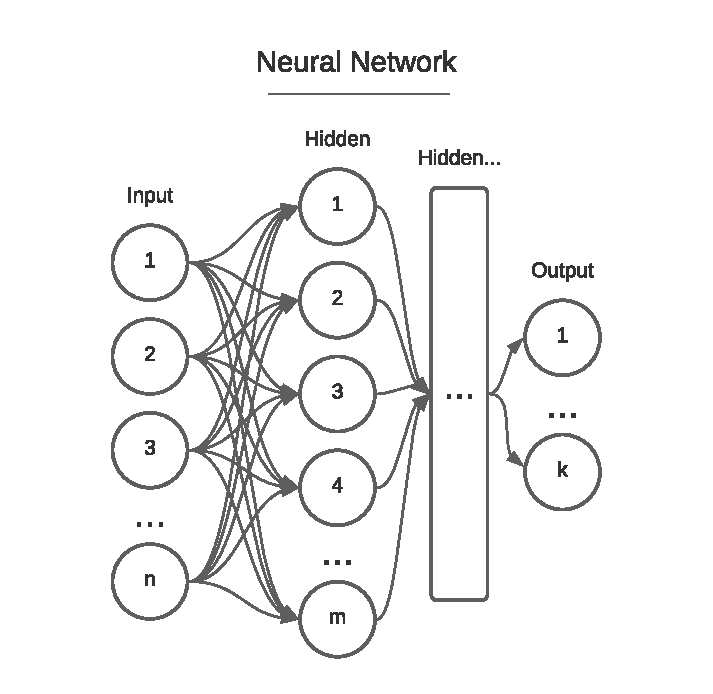
\includegraphics[width=0.8 \textwidth]{Figures/Neural-Network.pdf}
    \caption{An example diagram of basic neural network structure.}
    \label{fig:rl:nn}
\end{figure}

As noted in Chapter \ref{chap:intro}, deep learning techniques based on neural networks \cite{deepmind2020go} \cite{deepmind2020alphafold2} have been widely praised and covered in the media. Deep learning is not practical for use in this project as the size of the data set is too small (Chapter \ref{chap:data}). 

Smaller neural networks can be employed on the DI data.
However, even smaller networks can be hard to interpret, as seen in Figure \ref{fig:rl:nn} the nodes of a neural network are all deeply interconnected. This interconnection is powerful in that it enables the network to create complicated features based on the data during training. These complicated features are double-edged, because they can allow for higher classification performance, but can make it nearly impossible for a human to determine how a classification decision was made. In the simple case of a network with one or two layers and a reasonable number of nodes, it is possible to inspect the network and determine how classifications are made. However, as the number of layers and nodes increases, this power is lost.
Techniques, such as LIME \cite{ribeiro2016lime} \cite{vanberlo2020interpretable} \cite{lundberg2017shap}, have been proposed as a tool that helps overcome the interpretability issue. However, this technique and others like it only help explain why a neural network-based classifier made the classifications it did, they do not help interpret the inner workings of the network itself. 



\section{Decision Trees and Random Forests} \label{chap:rl:tree}
Decision (and regression) trees are another popular tool for creating interpretable models \cite{friedman2001greedy} \cite{chen2016xgboost} \cite{chan2017evidence} \cite{kube2019allocating}. Decision trees start from a single root proposition, such as "Will become chronic?", and iteratively create divisions until the root proposition can be answered with some given degree of certainty. Figure \ref{fig:example-decision-tree} demonstrates the structure of a decision tree. This tree structure makes models immediately interpretable, either by presenting the tree or breaking the tree down into rules of the form "Will become chronic if feature A and feature B". This transparency fades when the tree becomes very large. However, this is usually not an issue as large trees suffer from over-fitting. Over-fitting is the result of a machine learning system that learns patterns in a training population that do not extend to the broader population. This results in poor real world performance and makes over-fitting something to be avoided. Decision trees also suffer from the issue of feature ordering. Tree models are fit by "growing" the tree downwards, meaning the order of feature evaluation is fixed during growth, which can result in a sub-optimal tree structure.
Random forests are a method \cite{toros2019early} that overcome this problem by building an ensemble of decision trees. Random forests make a classification decision by taking a vote of confidence from all trees in the forest, this also helps alleviate the over-fitting problem with decision trees. While random forests are in general a marked improvement over decision trees, they lose the interpretability.

\begin{figure}[ht]
    \centering
    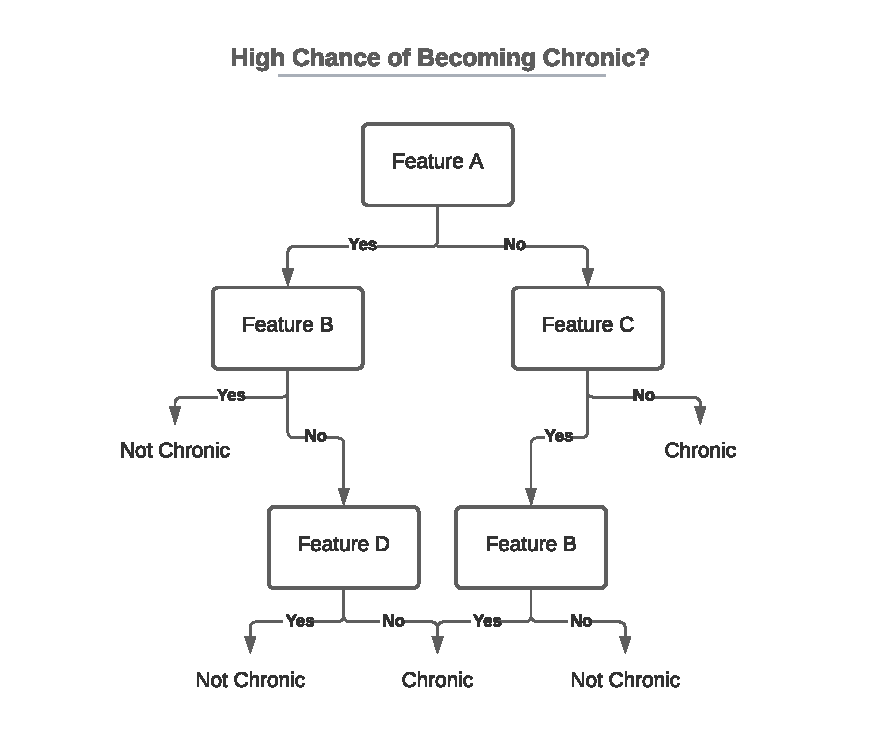
\includegraphics[width=1\textwidth]{Figures/Decision-Tree-Example.pdf}
    \caption{A diagram displaying the structure of a decision tree.}
    \label{fig:example-decision-tree}
\end{figure}

\section{Logistic Regression} \label{chap:rl:lr}
By far the most popular predictive tool in the homeless space is Logistic Regression \cite{hastie2009elements} \cite{king2001LogisticR} \cite{allegheny2019homeless} \cite{hong2018applications} \cite{toros2019early}. Logistic regression is a binary predictor that assumes a combination of feature variables have a linear relationship with the log-odds of an event. Historically, this has been popular because the simple definition lends itself well to interpreting (linear) relationships. Logistic regression is defined as $\log \frac {p}{1-p} = \beta_0 + \beta_1 f_0 + \beta_2 f_1 ...$ where $p$ is the probability of event, $f_n$ are the features based on the data set, and $\beta_n$ are the parameters of the model. The parameter values ($\beta_n$) can be used after training to demonstrate a feature's impact on the classification, leading to a model with a fairly large degree of interpretability.
Logistic regression falls short in two places. First, the model is interpretable for users with the right set of tools, however, the layperson (e.g. front-line shelter staff) is left to trust in parameter values often without the math background to have confidence in the model. Second, the algorithm has a necessary assumption that the data is linearly related, which limits the insights that can be generated. This can be mitigated to a degree by adding new features that are non-linear combinations of existing features, but this method would damage the  interpretability of the model.


% \section{Survival analysis} \label{chap:rl:survival}
% \tdo{Finish the survival analysis section}
% There are also similar algorithms used for regression. Notably in this space is Cox proportional hazards regression \cite{greer2016targeting} \cite{Kim2009UnstableHA}, which is used to calculate some risk value corresponding to the likelihood of a client entering/re-entering homelessness. This technique is especially popular in the homeless space, as it provides an approximate "time to event" rather than a binary flag. 


 \chapter {Data} \label{chap:data}


This chapter will introduce the data provided by the DI, and the processing steps necessary to anonymize and prepare the data for use in classification rule learning.
Section \ref{chap:data:cleaning} details the anonymization and bias-removal steps.
Next, Section \ref{chap:data:layout} introduces a naming convention and describes the format of the data before and after the initial aggregation. Section \ref{chap:data:labelling} will detail the chronic label.

\section{Data Anonymization and Cleaning} \label{chap:data:cleaning}

This work was carried out using data collected at the DI between July 1, 2007, and January 20, 2020. The data set contains 34,577 unique clients with a total of 5,393,987 recorded interactions with the DI. The data is organized into one table that covers all clients. Each row of the table contains a single interaction with the shelter, which can be a sleep event, a meeting with a counsellor (addiction services, career services, etc.), a log of some interaction, or an event resulting in a variable-length ban. Interactions have a timestamp, a unique client ID and a unique table index.
The data anonymization and a client privacy protocols used in this work were approved by the University of Calgary Conjoint Faculties Research Ethics Board. 
Following the procedure put forth by Kuhn and Culhane \cite{kuhn1998applying}, the data was pruned to mitigate the effects of left-truncation and right-censor bias.

Censoring is the effect that comes from the discrete start and end of data collection.  That is, a client who accesses shelter services before July 1, 2007, will have the initial portion of their access records missing. Any client who is not identified as chronic prior to January 20, 2018, will be potentially mislabeled because they could become chronic after January 20, 2018. These effects are called left-truncation bias and right-censor bias respectively.

Left-truncation bias results from the sharp cut-off at the start of data collection.
In the context of this work, there will be individuals who are chronic at the start of the data collection but any analysis will not see this and determine that the individual is a new client. The DI started collecting sleep records on July 1, 2008, thus we set the left-truncation bias cut-off to July 1, 2009, and remove any client that slept at the DI before that date. The assumption is that clients within one year of the start of data collection have a higher probability of having accessed DI services prior to the beginning of data collection.

Right-censor bias is a result of filtering clients who continue to access the shelter after the end of the data record. These clients might become chronic after the end of the available data, meaning any system is likely to classify them incorrectly. Thus we set the right-censor bias cut-off to January 20, 2018.

When performing the right-censor bias adjustment there are two appropriate methods. The first being to remove all clients that have a recorded interaction after the cut-off date. The other is to remove only the clients who have their first interaction (in this work, sleep interactions were used) after the cut-off date. The first method minimizes the number of individuals who become chronic that are mislabelled as not chronic at the cost of having fewer individuals in the data set. The second method retains more individuals in the data set but has a higher risk of mislabelling a few individuals. In this work, the second method was used as it resulted in a larger number of identified chronic individuals.

% Fortunately, these methods can be compared using historical data. As with the main work, this analysis will be performed using data after the censor bias mitigation efforts, with cut-off dates of July 1, 2009 and January 20, 2018 for the left-truncation and right-censor respectively. 

% To properly compare these two methods, it is necessary to make an estimate of the false non-chronic count using the first method and the additional true-chronic individuals identified using the second method. The latter value is much easier to calculate as it is simply the difference between the number of classified individuals when using each method. Performing this simple analysis tells us that there is a difference of 593 clients identified as chronic (884 vs 291).

% Estimating the false non-chronic count is more difficult. Individuals that are falsely classified as non-chronic because of the right censor bias, are those who eventually become chronic after the data collection date (January 20, 2020), with the cut-off date set to 2018. Which gives clients two years to become chronic in the worst case (the worst case is a client who first accesses shelter services in January 19, 2018). Using this we can generate an approximate upper bound on the number of missed clients.

% The upper bound can be estimated by observing the probability that an individual is identified as chronic after two or more years, and making the assumption that all clients from some period prior to January 20, 2018 all enter for the first time on January 19, 2020. For this work we will look at the period from January 20, 2016 - January 19, 2018. This includes a total of 5208 clients. Over the entire data set it was observed that \~1.84\% of clients become chronic after two or more years. Which gives the upper bound of $5208 \cdot 0.184 = 96 \text{ individuals}$ . A lower bound can be similarly computer by assuming all 5208 clients entered on January 20, 2016. ~0.818\% of clients become first chronic after four years, applying this gives  $5208 \cdot 0.0818 = 43 \text{ individuals}$ . 

% Finally, comparing the two methods it is observed that the first method results in 593 fewer identified chronic clients (a reduction of 67\%) but results in upwards of 100 fewer mis-classified individuals. In this work, the second method will be used, as having more than three times as many chronic individuals identified will help the learning algorithm.

Thus, any client that starts sleeping at the DI after January 20, 2018, is removed from the data set.
This reduced the clients covered down to 18,398, representing a 46.8\% reduction in the number of clients.



\section{Data Layout and Transformations} \label{chap:data:layout}

% Original (RAW) data table $T$
% Client data table (These are called attributes) $A$ (num_df)
% Individual attributes are labelled $a_1, a_2, ..., a_L$
% Coverage Table (features) $\mathcal{F}$
% Each column represents a feature (/single rule) $f_i$
% class labels (true/false) $c$
% predicted labels $\hat c$

\subsection{DI Data Table}


The data collected at the DI comes as one data table $T$, where columns contain data points being tracked (e.g. ClientID) and each row contains one interaction with the DI for a total of 2,184,854 interactions. Table \ref{tbl:university} outlines each column and the type of data that it can contain. The EntryType column details why each event was logged. For example, an EntryType of Bar is recording that the client was banned from the DI on that specific day. The Bar duration is not used in this work. Similarly CounsellorsNotes, ProgressDetails, and Log correspond to three different instances of entering a written log into the database. For privacy reasons the log text is not used. Sleep events occur when a client accesses the DI to sleep.


\begin{table}[h!]
	\begin{tabular}{ c c p{0.7\textwidth} } 
		\toprule
		Column name & Values &  \\
		\midrule
		ClientId & \emph{integer} & Unique to each client \\
		Date & \emph{date} & Date of interaction \\
		Age & \emph{integer} & Client's age at the time of data export \\
		EntryType & \emph{string} & One of 'Bar', 'CounsellorsNotes', 'ProgressDetails', 'Log', 'Sleep' \\
		EmployeeIsCounsellor & \emph{boolean} & Is the employee logging the interaction a counsellor? \\
		EmsLogFlag & \emph{boolean} & Were EMS called for this client? \\
		PoliceLogFlag & \emph{boolean} & Were the police called on account of this client? \\
		\bottomrule
	\end{tabular}
	\caption{Description of data ($T$) provided by the DI.}
	\label{tbl:university}
\end{table}


Missing or invalid data can introduce a large amount of error in the final classifications, and it is thus necessary to discuss what is done when presented with missing or invalid data. The data used in this work has been exported from the DI after having undergone some preliminary cleaning. The cleaning was performed before being exported at the DI, the raw data was not observed in this work. This means the data $T$ can be trusted to only contain valid values (e.g. all counts are positive, there are no null values, etc.). 

Another source of potential bias is the existence of the diversion services team at the DI. This team is responsible for identifying chronic individuals and individuals at risk for chronic homelessness and helps transition them into housing following housing first principles. This is considered to be a small source of bias in this work as the diversion services team is relatively new. Housing first in Canada was heavily influenced by the At Home/Chez Sois study which concluded in 2014 \cite{athome2014chezsoi}.

\subsection{Data Transformations}

The data format described above is not sufficient for use with our classification rule learning system and is not yet suitable to perform all but the most basic analysis. A better format would be a table where each client is a row and each column is an attribute describing the client.
This new table is called $A$ and has a length of 18,398 (the total number of clients).
Each attribute of $A$ is denoted $a$, where $a_i$ denotes the $i$th column name of $A$. The minimum and maximum values of attribute $a$ are denoted $min(a)$ and $max(a)$ respectively. Each attribute $a$ is a summary of interactions that a client has recorded in $T$. For example, a common attribute is 'Sleep' which records the total number of times a client has an EntryType of Sleep in $T$.
The table $A$ has nine columns (attributes), Age, Bars, CounsellorsNotes, EmployeeIsCounsellor, EmsLogFlag, Log, PoliceLogFlag, ProgressDetails, Sleep.



The nine columns of $A$ are derived from the seven columns in $T$. Not all the columns in $T$ are directly used as attributes. Some columns are combined to create an attribute. For example, the Date column does not become an attribute but is used together with the Age column to calculate a client's age at the first interaction with the DI.
The Age column in $T$ represents client age when the data was exported (2020). To get the actual age at the time of interaction, the Date field is used to calculate the client's approximate age. As a matter of anonymity, the client's birth dates are unknown, which means the Age attribute is only accurate to one year.
The EntryType column is a categorical column with five options 'Bar', 'CounsellorsNotes', 'ProgressDetails', 'Log', and 'Sleep'. This column is split into five attributes with each attribute counting the number of times a client had an EntryType equal to that attribute.
The EmployeeIsCounsellor, EmsLogFlag, and PoliceLogFlag columns each become separate attributes that count the number of times these flags were set in $T$.


As the purpose of this work is to classify individuals as soon as possible, the entire attribute table will not be used when making classifications. Instead, a modified attribute table will be used that is generated using only a client's first $d$ days after first sleeping at the DI. 
This is fortunately a simple procedure. Instead of making the transformation of $T \rightarrow A$ an additional procedure that filters out client interactions $d$ days after the client's first sleep is introduced. The new transformation is $T \rightarrow A_d$ where $A_d$ represents the attribute table for each client's first $d$ days after sleeping at the DI. For example, the attribute table that represents a client's first 14 since sleeping at the DI is denoted $A_{14}$.

 The $A_d$ table has an additional seven columns, which represent the count of the non-sleep and non-age attributes prior to a clients first sleep at the DI. This means the $A_d$ table has 16 columns Age, Bars, CounsellorsNotes, EmployeeIsCounsellor, EmsLogFlag, Log, PoliceLogFlag, ProgressDetails, Sleep, Bars\_before, CounsellorsNotes\_before, EmployeeIsCounsellor\_before, EmsLogFlag\_before, Log\_before, PoliceLogFlag\_before, and ProgressDetails\_before.


\subsection{Exploratory Data Analysis} \label{chap:data:characteristics}

The attribute table $A_d$ introduced in the previous section is in a form that makes a basic exploratory data analysis possible. For this exploratory data analysis, a $d$ of 30,000 days is used. 30,000 days is larger than the entire data set, so the attribute table $A_{30,000}$ will include all data about a client from their first sleep, until the last day of available data.

Table \ref{tbl:stats:notchronic} includes a summary of the nine attributes along with five additional fields, here called demographics. These fields are Interactions, Tenure, Usage, Average Gap Length, and Episodes. Interactions are a simple count of each recorded interaction a client has with the DI (all EntryTypes). Tenure is the total number of days between a client's first and last interaction with the DI. Usage is the percentage of days that a client accesses DI services, a high usage is indicative of a heavy shelter user, or an individual with a short homeless stint. Average Gap Length is the average gap between stays at the DI, a low Average Gap Length can indicate a heavy user of DI services. Episodes track a client's total number of homeless episodes, where an episode is a grouping of shelter sleeps with a gap between sleeps not exceeding 30 days.

It can be seen from Table \ref{tbl:stats:notchronic} that, while there is a large range of values from each attribute (and demographic), most client experiences are grouped toward the lower end. Figures \ref{fig:pdf} and \ref{fig:demopdf} demonstrate the distribution of these values. This reinforces that the majority of clients that access shelter services only do so a small number of times, in fact, Figure \ref{fig:pdf} shows that the vast majority of clients spend less than 10 nights sleeping at the DI.


\begin{table}[h]
	\centering

	\begin{tabular}{lrrrr}
	\toprule
	Attributes													 &        min &   max &     mean &   median \\
	\midrule
	Age                          &          0 &   119 &    38.79 &       37 \\
	Bar (Count)                  &          0 &    68 &     1.05 &        0 \\
	CounsellorsNotes (Count)     &          0 &   443 &     3.72 &        0 \\
	EmployeeIsCounsellor (Count) &          0 &   464 &     6.25 &        0 \\
	EmsLogFlag (Count)           &          0 &    27 &     0.12 &        0 \\
	Log (Count)                  &          0 &  2419 &     7.23 &        0 \\
	PoliceLogFlag (Count)        &          0 &    23 &     0.13 &        0 \\
	ProgressDetails (Count)      &          0 &   539 &     4.77 &        0 \\
	Sleep (Count)                &          1 &  3575 &    82.95 &        5 \\
	\midrule
	Demographics								 &         &    &      &    \\
	\midrule
	Interactions (Count)         &          1 &  5247 &   118.75 &      8.0 \\
	Tenure (Days)                &          1 &  3800 &  650.526 &      138 \\
	Usage (\%)                    &  0.0541859 &   100 &  48.5072 &  34.0721 \\
	Average Gap Length (Days)    &          1 &  3690 &  135.634 &    11.25 \\
	% Stays (Count)                &          1 &  3575 &   82.949 &        5 \\
	Episodes (Count)             &          1 &    31 &  2.74611 &        2 \\
	\bottomrule
	\end{tabular}

	\caption{Basic Attribute statistics and Demographic data for the entire population.}
	\label{tbl:stats:notchronic}
\end{table}

\begin{figure}[ht]
  \figuretitle{Attribute Histograms}
  \centering

	\begin{subfigure}[b]{0.3\textwidth}
    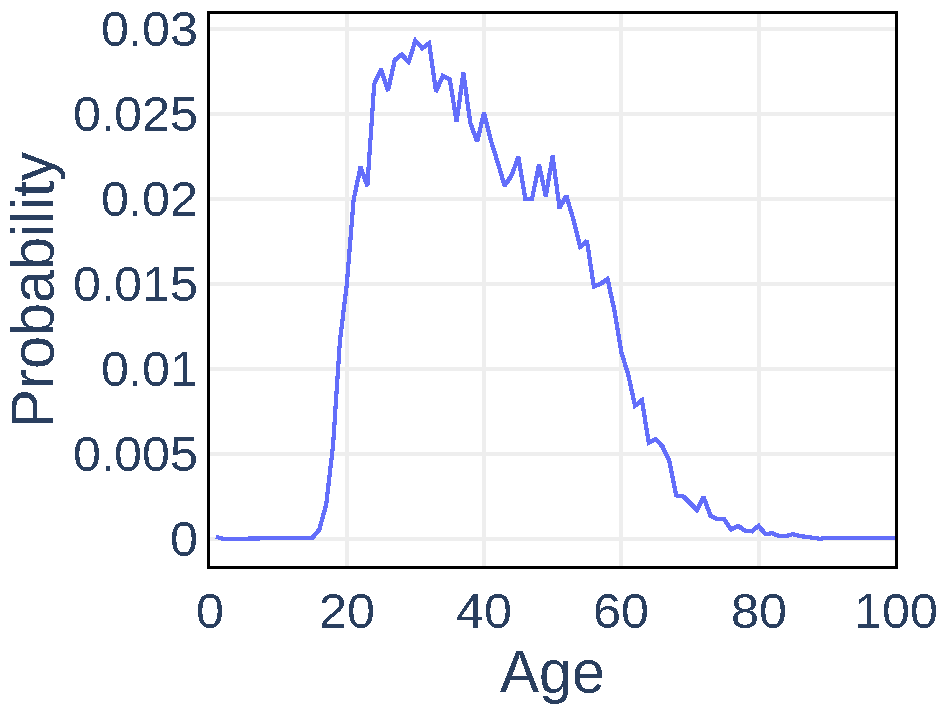
\includegraphics[width=\textwidth]{Figures/Data-Age-PDF}
  \end{subfigure}
	\begin{subfigure}[b]{0.3\textwidth}
    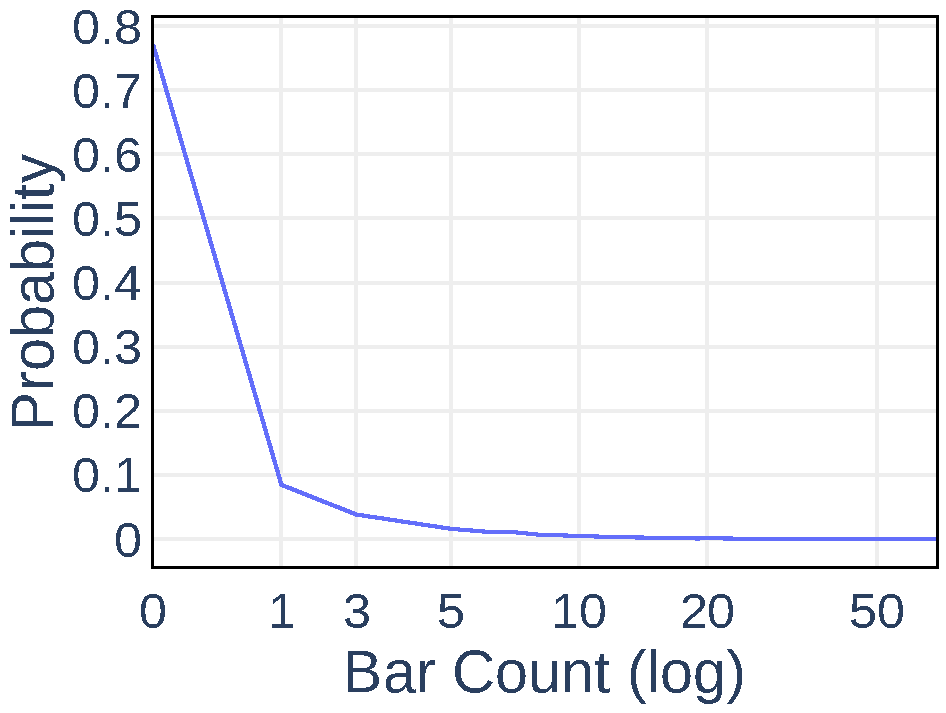
\includegraphics[width=\textwidth]{Figures/Data-Bar-PDF}
  \end{subfigure}
	\begin{subfigure}[b]{0.3\textwidth}
    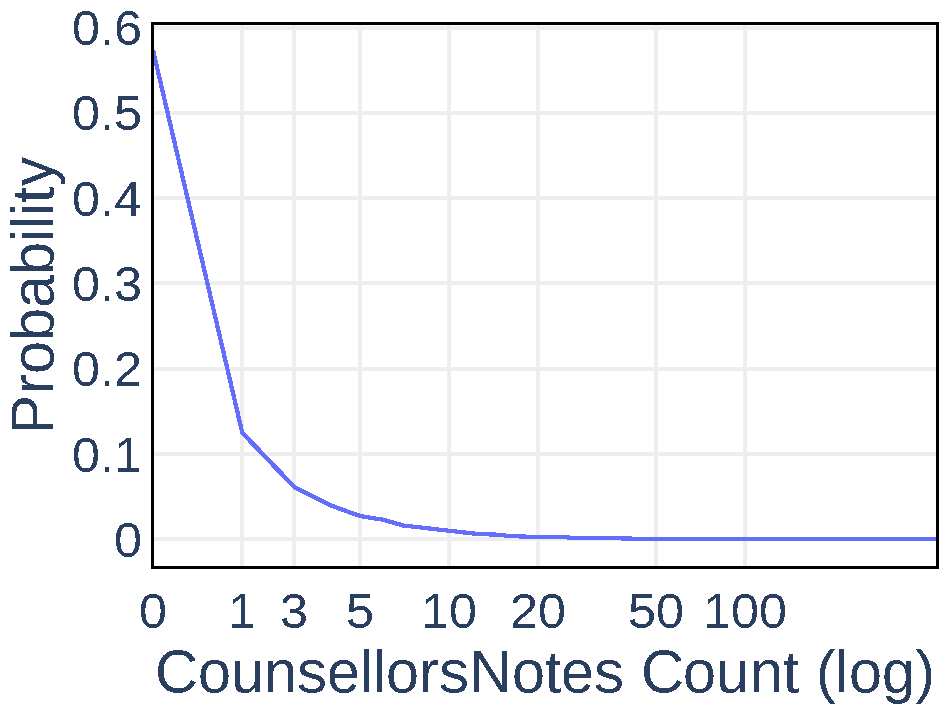
\includegraphics[width=\textwidth]{Figures/Data-CounsellorsNotes-PDF}
  \end{subfigure}
	\vspace*{1em}

	\begin{subfigure}[b]{0.3\textwidth}
    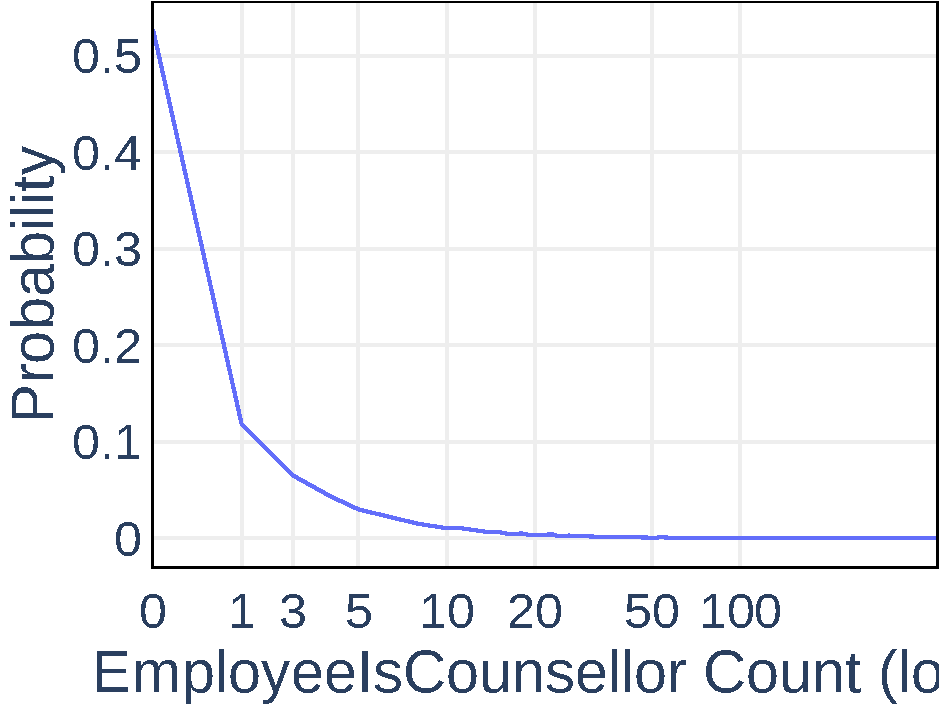
\includegraphics[width=\textwidth]{Figures/Data-EmployeeIsCounsellor-PDF}
  \end{subfigure}
	\begin{subfigure}[b]{0.3\textwidth}
    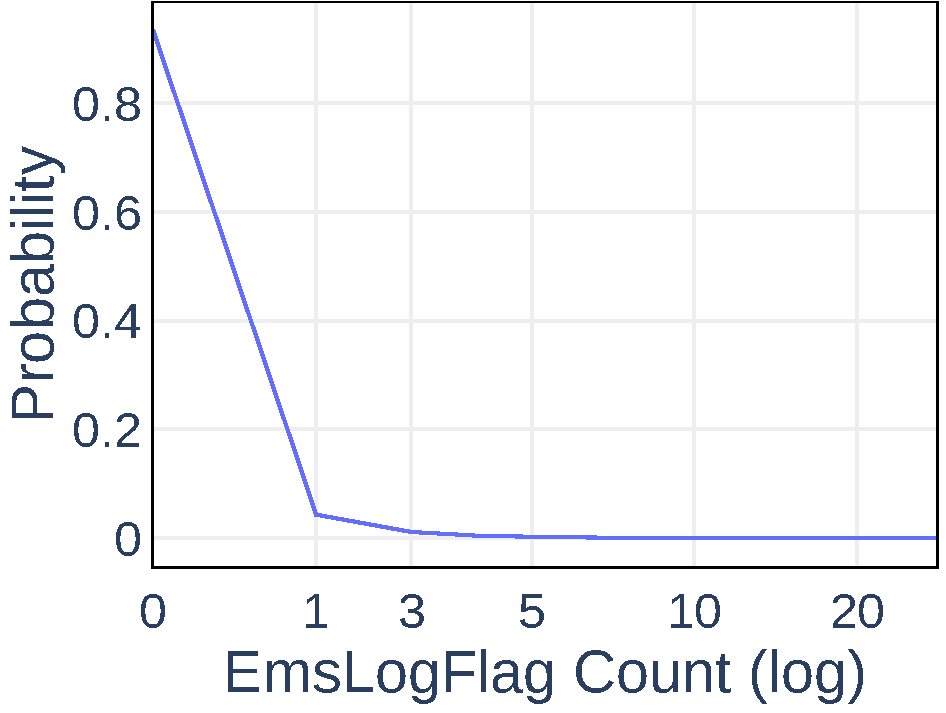
\includegraphics[width=\textwidth]{Figures/Data-EmsLogFlag-PDF}
  \end{subfigure}
	\begin{subfigure}[b]{0.3\textwidth}
    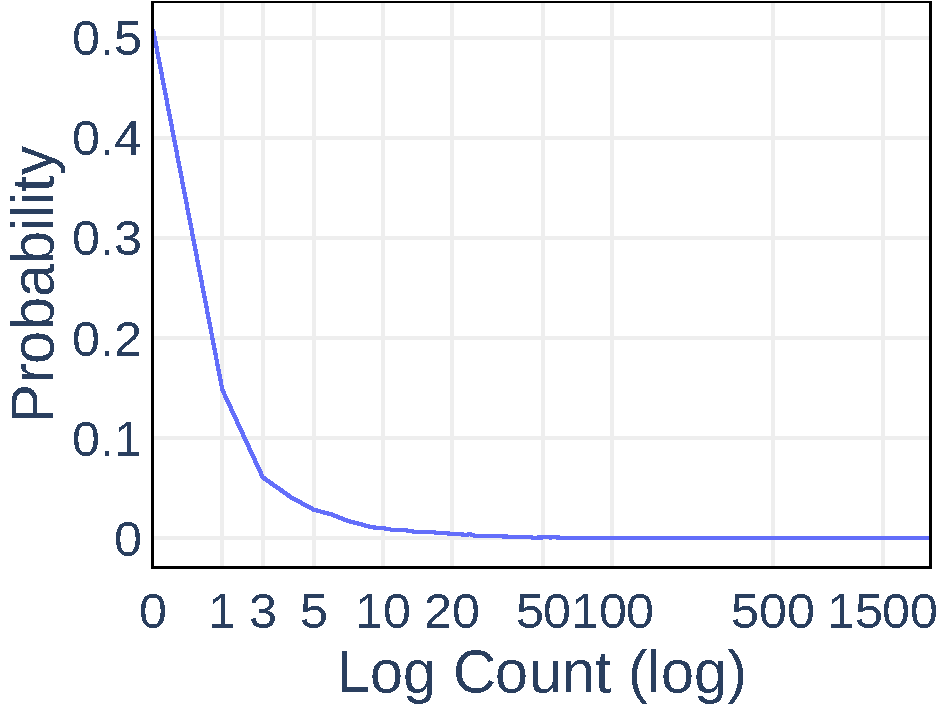
\includegraphics[width=\textwidth]{Figures/Data-Log-PDF}
  \end{subfigure}
	\vspace*{1em}

	\begin{subfigure}[b]{0.3\textwidth}
    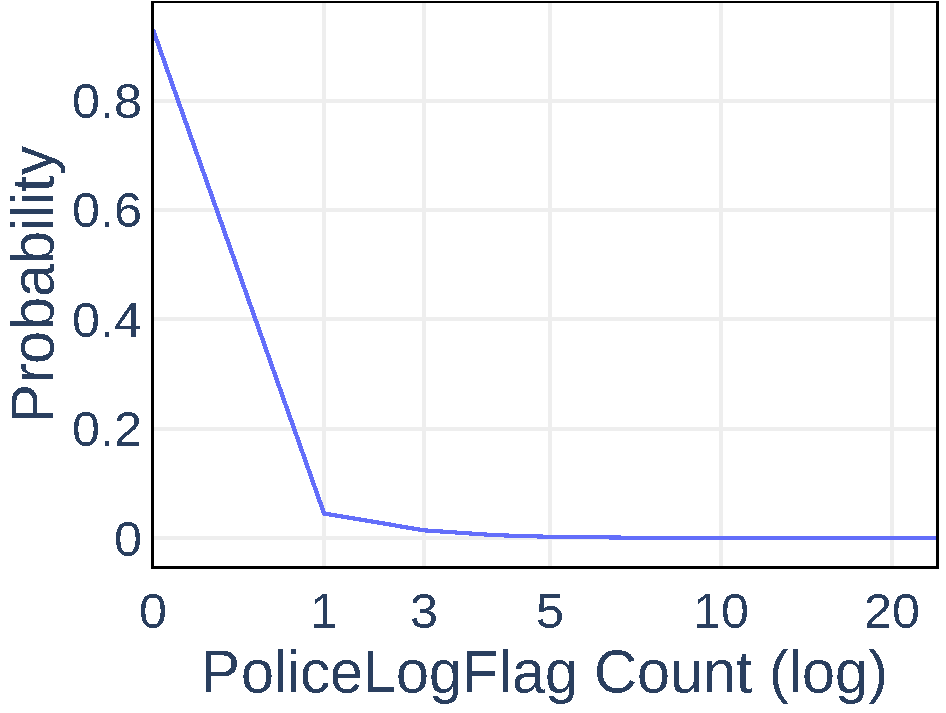
\includegraphics[width=\textwidth]{Figures/Data-PoliceLogFlag-PDF}
  \end{subfigure}
	\begin{subfigure}[b]{0.3\textwidth}
    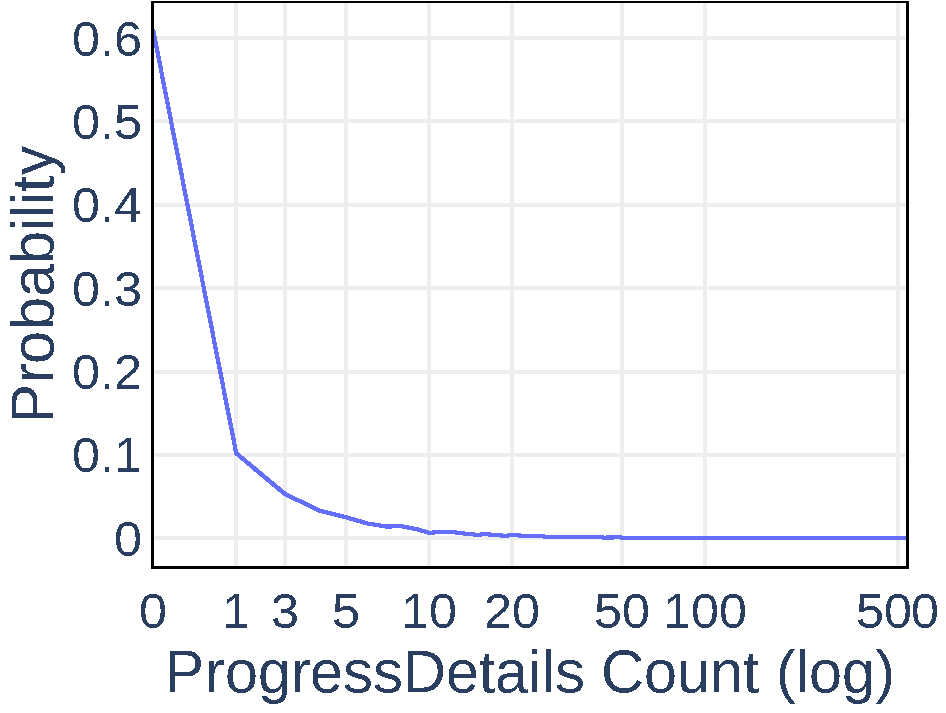
\includegraphics[width=\textwidth]{Figures/Data-ProgressDetails-PDF}
  \end{subfigure}
	\begin{subfigure}[b]{0.3\textwidth}
    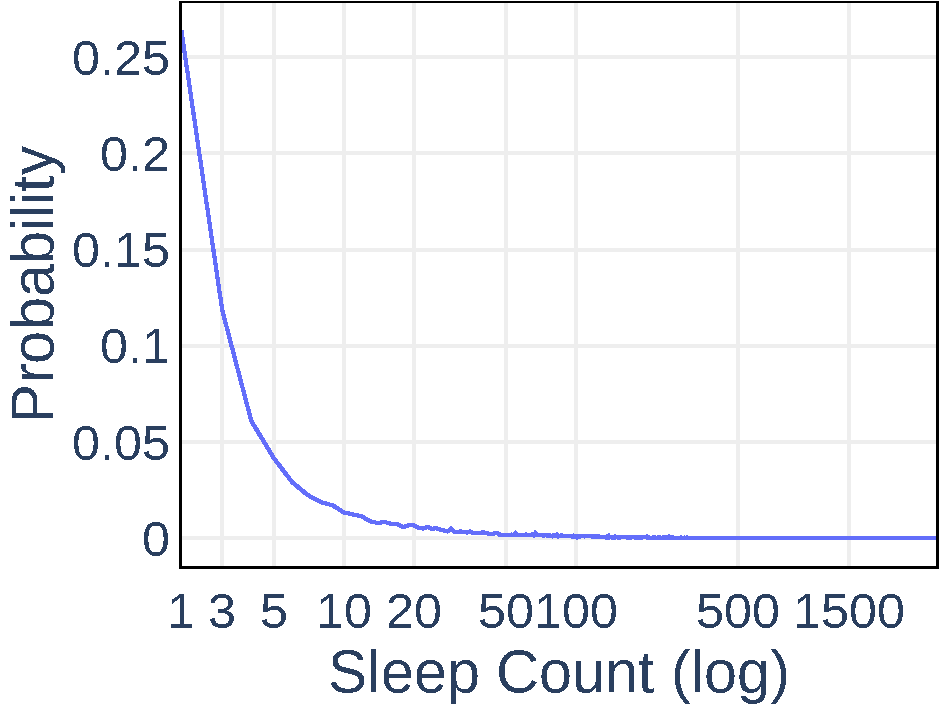
\includegraphics[width=\textwidth]{Figures/Data-Sleep-PDF}
  \end{subfigure}
	\caption{Histograms of the nine attributes.}
	\label{fig:pdf}
\end{figure}

\begin{figure}[ht]
  \figuretitle{Demographic Histograms}
  \centering

	\begin{subfigure}[b]{0.3\textwidth}
    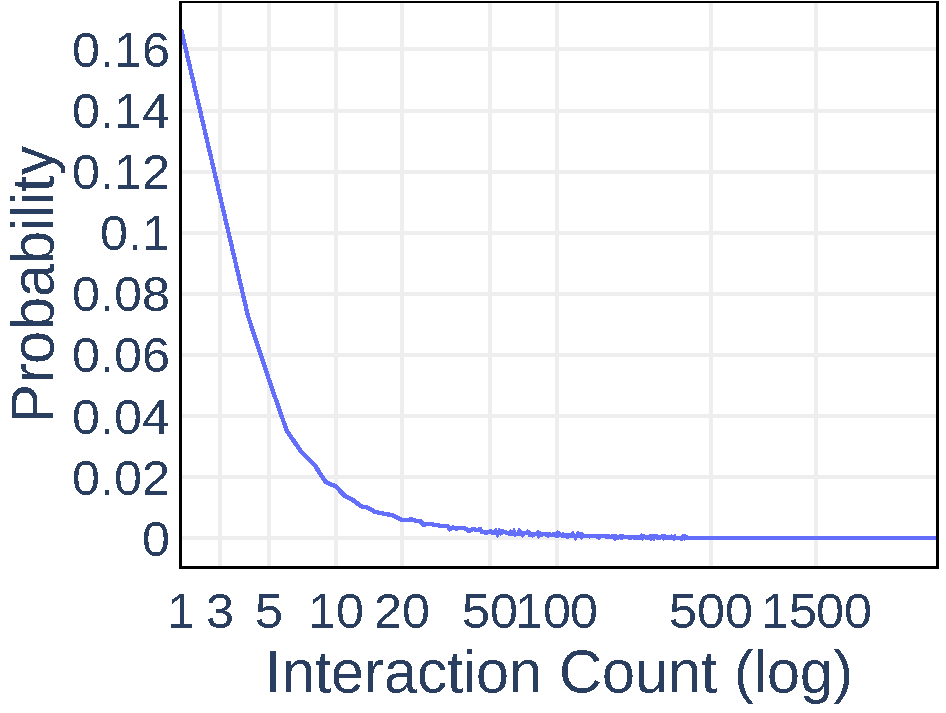
\includegraphics[width=\textwidth]{Figures/Data-Interaction-PDF}
  \end{subfigure}
	\begin{subfigure}[b]{0.3\textwidth}
    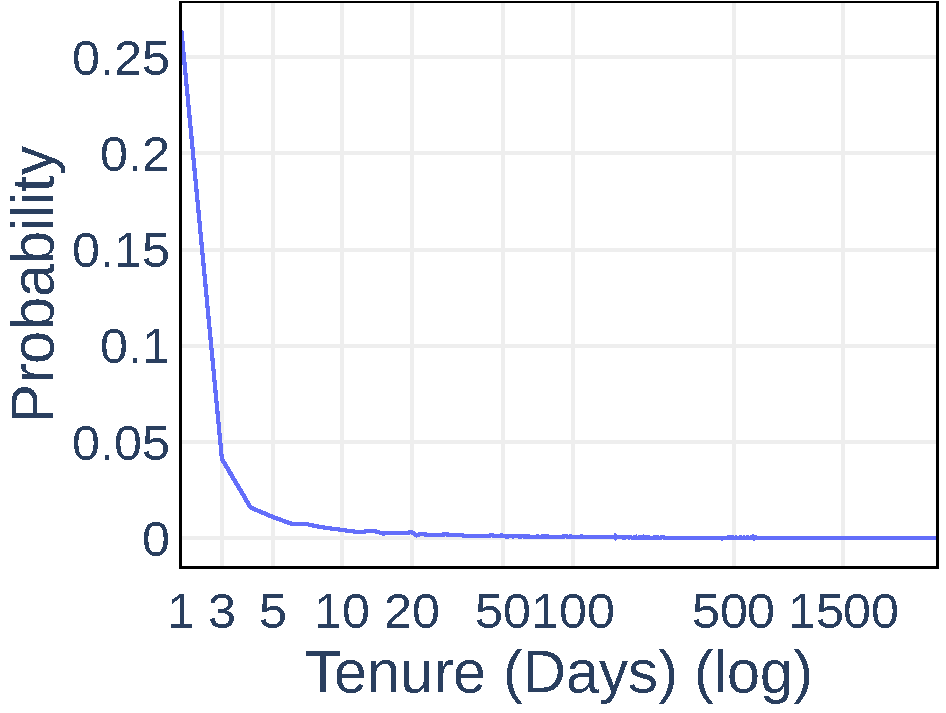
\includegraphics[width=\textwidth]{Figures/Data-Tenure-PDF}
  \end{subfigure}
	\begin{subfigure}[b]{0.3\textwidth}
    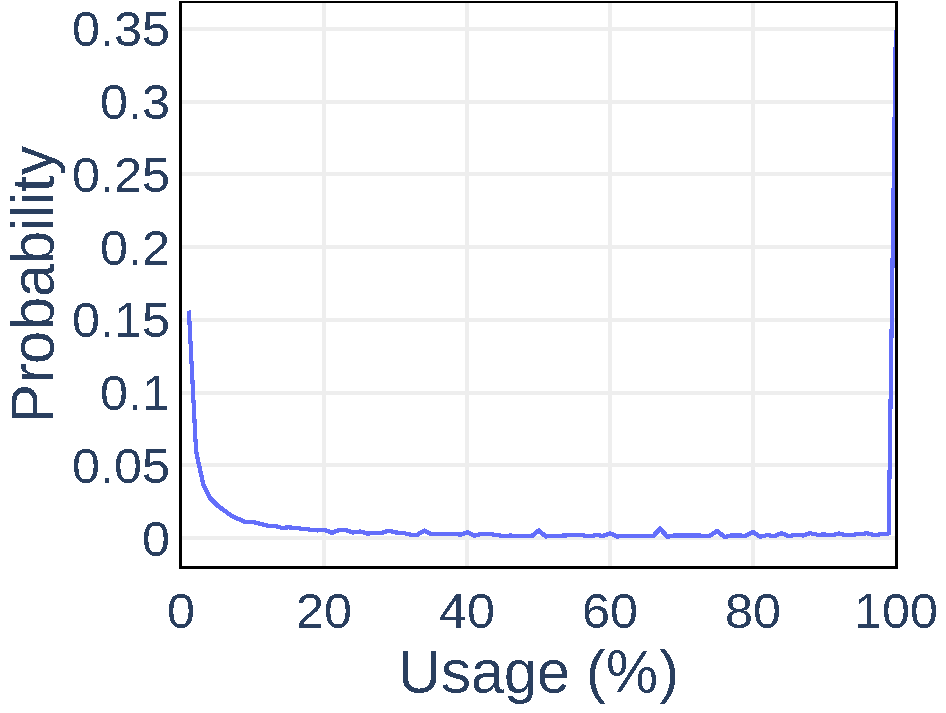
\includegraphics[width=\textwidth]{Figures/Data-UsagePct-PDF}
  \end{subfigure}
	\vspace*{1em}

	\begin{subfigure}[b]{0.3\textwidth}
    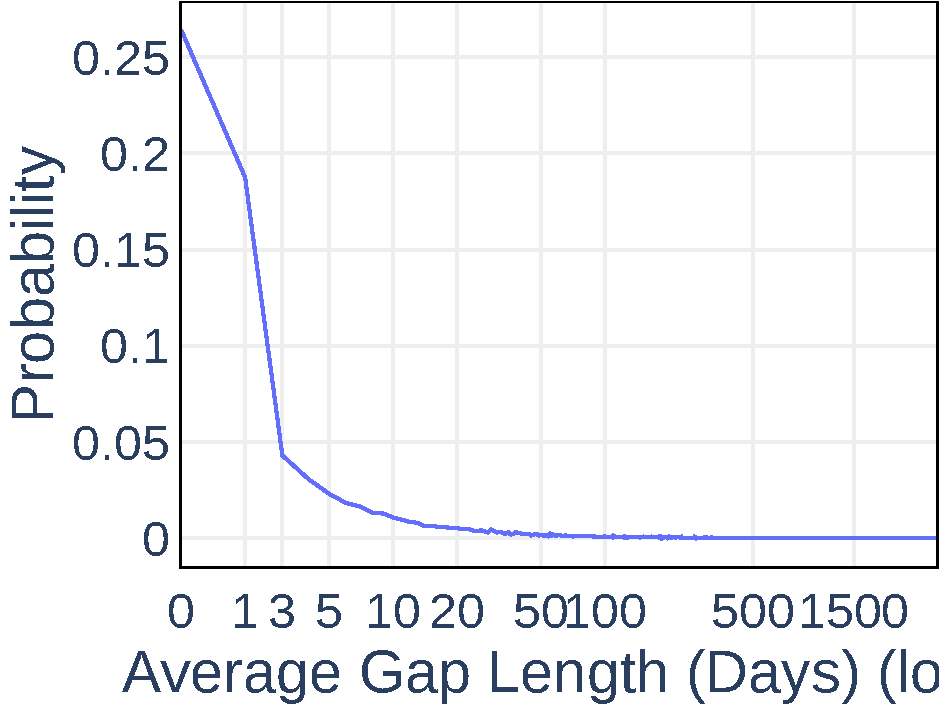
\includegraphics[width=\textwidth]{Figures/Data-AvgGapLen-PDF}
  \end{subfigure}
	% \begin{subfigure}[b]{0.3\textwidth}
    % 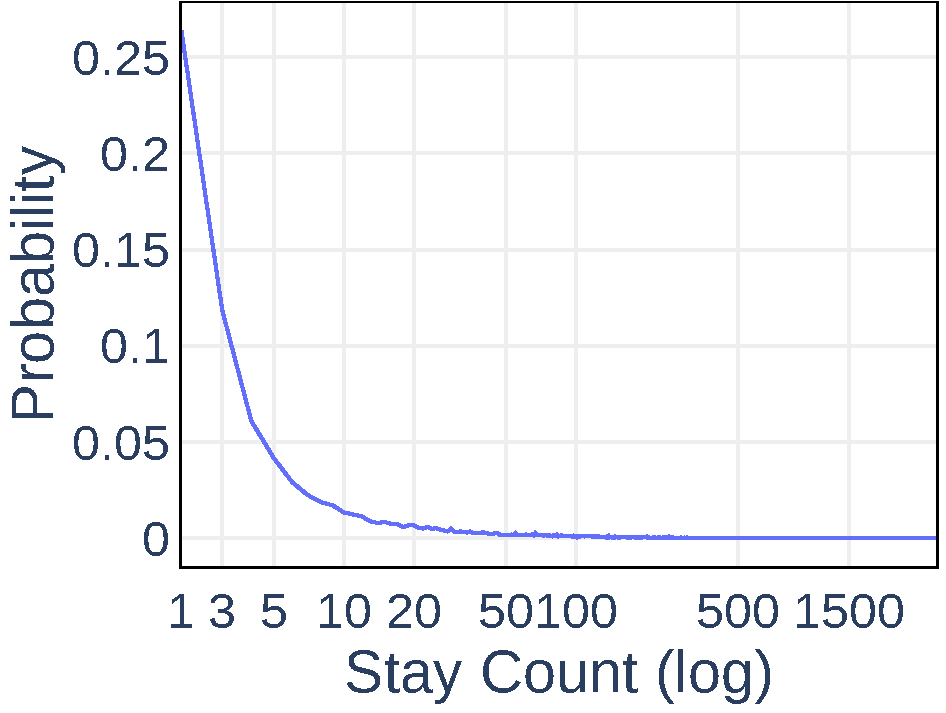
\includegraphics[width=\textwidth]{Figures/Data-TotalStays-PDF}
  % \end{subfigure}
	\begin{subfigure}[b]{0.3\textwidth}
    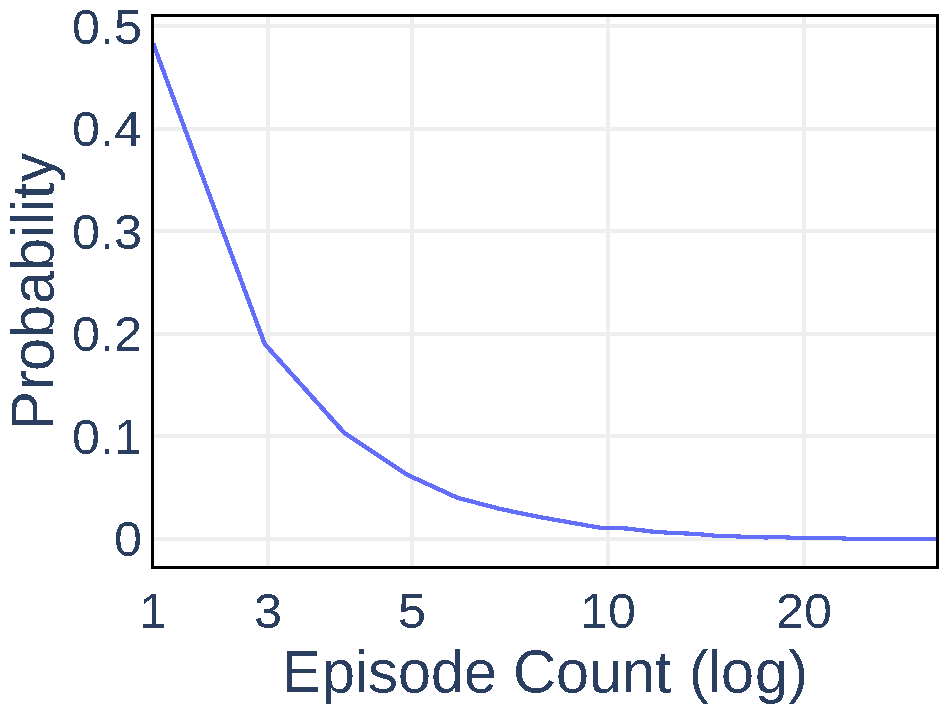
\includegraphics[width=\textwidth]{Figures/Data-TotalEpisodes-PDF}
  \end{subfigure}
	\caption{Histograms of the five Demographic fields.}
	\label{fig:demopdf}
\end{figure}


\section{Labelling the Data} \label{chap:data:labelling}

As stated in the introduction, the approach taken in this work is to identify clients that will eventually become chronic. There is no consensus for what it means to be chronically homeless, thus a definition must be selected. There are three "standards" that apply to our work, the Canadian federal definition, the Alberta provincial definition, and the definition applied by the DI. There are also several standards \cite{byrne2015testing} from other locations and organizations which will not be considered here. The three definitions under consideration are:

\begin{enumerate}
\item \textbf{Government of Canada (GoC):} "individuals who are currently experiencing homelessness AND who meet at least 1 of the following criteria: they have a total of at least 6 months (180 days) of homelessness over the past year or they have recurrent experiences of homelessness over the past 3 years, with a cumulative duration of at least 18 months (546 days)" \cite{canada2020definition}
\item \textbf{Government of Alberta (GoA):} "A person or family is considered chronically homeless if they have either been continuously homeless for a year or more, or have had at least four episodes of homelessness in the past three years." \cite{snyder2008albertadefinition}
\item \textbf{Calgary Drop-In Centre (DI):} "individuals who access the Calgary Drop-In Centre more than 75\% or 276 [sic] days in a calendar year" \cite{di_2019}.
\end{enumerate}

Of these three definitions, the DI definition was selected for use in this work. It was selected for two reasons. First, the DI definition most closely aligns with the original chronic classification \cite{kuhn1998applying}, as shown in our other work \cite{messier2020}. The second, and perhaps more functional reason, is that this work is being undertaken in partnership with the DI, and thus will use the internal definition of the DI.

Thus, for the remainder of this thesis, the term "chronic" will refer to chronic under the DI definition. In the context of homelessness, we interpret "access" as sleeps and do not include access to other DI services (which can be available to housed individuals). It is possible for a client to access the DI for both day and night sleeps, in this definition only a maximum of one sleep per 24 hour period is counted. Our analysis will be constrained to clients that spend at least one night (or day sleep) at the shelter. Of the 18,398 clients covered by this data set, only 886 (4.82\%) have ever met the DI definition for chronic homelessness.

The chronic label generated by applying the DI definition across the attribute table $A$ will be denoted $C$. Thus $C$ is a vector of boolean values corresponding to the chronic status of each client in $A$. To generate $C$ a rolling window of 365 days is applied to each client in $T$. The number of unique sleeps within any of those resulting windows is counted and if this number is greater than or equal to 276 nights, the client is identified as having experienced chronic homelessness. We note that this definition requires a recently homeless person to spend \emph{at least} 276 days sleeping in a shelter before being eligible for additional support based on chronic status.
While the minimum required time to be identified as chronic is 276 days, the median is 349 days and the mean is 666 days. These numbers are based on the data provided to us by the DI.
This effect was studied in our previous work \cite{messier2020} and motivates the need for a tool that considers a client's first $d$ days in shelter, where $d < 276$. $C$ will be used in later chapters as the class label for training procedures.

\subsection{Characteristics of Chronic Clients}

Following the discussion in Section \ref{chap:data:characteristics}, the same table structure will be presented here focusing only on clients that were identified as chronic using the DI definition (Table \ref{tbl:stats:chronic}). It can be seen that the median client who meets the definition of chronic has significantly more interactions than the general population (Table \ref{tbl:stats:notchronic}). Furthermore, as could be expected, the minimum number of sleeps is 276, and the minimum tenure is only slightly higher at 280. A new row, Tenure Pre-chronic, has been added to demonstrate the number of days a client is homeless before being identified as chronic. 

\begin{table}[h]
	\centering

	\begin{tabular}{lrrrr}
	\toprule
	Attributes &      min &      max &     mean &   median \\
	\midrule
	Age                          &       19 &       83 &    51.67 &       54 \\
	Bar (Count)                  &        0 &       68 &     5.21 &        2 \\
	CounsellorsNotes (Count)     &        0 &      443 &    26.34 &       17 \\
	EmployeeIsCounsellor (Count) &        0 &      464 &    58.78 &       32 \\
	EmsLogFlag (Count)           &        0 &       27 &     0.73 &        0 \\
	Log (Count)                  &        0 &     2419 &    62.23 &       21 \\
	PoliceLogFlag (Count)        &        0 &       11 &     0.34 &        0 \\
	ProgressDetails (Count)      &        0 &      539 &    45.37 &       30 \\
	Sleep (Count)                &      276 &     3575 &   955.06 &    787.5 \\
	\midrule
	Demographics								 &         &    &      &    \\
	\midrule
	Interactions (Count)         &      283 &     5247 &  1292.97 &   1091.0 \\
	Tenure (Days)                &      280 &     3800 &  1687.09 &     1636 \\
	Usage (\%)                    &  8.00225 &      100 &  63.6248 &  65.9663 \\
	Average Gap Length (Days)    &        1 &  12.5371 &  2.05862 &   1.5166 \\
	% Stays (Count)                &      276 &     3575 &  955.058 &    787.5 \\
	Episodes (Count)             &        1 &       22 &  3.69977 &        3 \\
	Tenure Pre-chronic (Days)    &      275 &     3623 &  665     &      349 \\
	\bottomrule
	\end{tabular}


	\caption{Basic Attribute statistics and Demographic data for chronic individuals.}
	\label{tbl:stats:chronic}
\end{table}


\section{Summary}

This chapter introduced the data set provided by the DI including the definitions used to label clients as chronic. Further, the attribute data and the demographic summaries were presented demonstrating some of the differences between chronic and non-chronic users of the DI. A discussion of classification evaluation measures will be presented in the following chapter.

 \chapter{Classification Rule Learning} \label{chap:rule}

Rule learning can be used in a supervised manner for classification, or in an unsupervised manner for knowledge discovery \cite{agrawal1996fast} \cite{kavvsek2006apriori}. In this work, rule learning is used for classification but takes cues from the other contexts.

This chapter will examine the individual parts of a rule learning system and present a popular implementation of classification rule learning. Section \ref{chap:rule:back} will provide an introduction to the architecture of a rule learning system.
Section \ref{chap:rule:ripper} will use this architecture to introduce the RIPPER \cite{cohen1995ripper} classification rule learner, which is perhaps the most famous rule learner. 
The specifics of the rule learning system used in this work will be detailed in Chapter \ref{chap:algo}.
This chapter provides a basic introduction into each section of classification rule learning, for a more in-depth introduction please see \cite{furnkranz2012foundations}.


\section{Background} \label{chap:rule:back}

The standard unit of rule learning is the \emph{rule}. A rule is an unordered combination of binary features that together restrict a population to a select few individuals that match each feature in the rule. A feature is a binary test that can be applied to the attribute matrix $A$ (defined in Section \ref{chap:data:layout}) that will categorize each client as "matching" the feature, or not.
As such, each attribute matrix will have a distinct set of features.
The set of all features will be denoted $\mathcal{F}$ where $\mathcal{F} = \{ f_1, f_2, ..., f_{|\mathcal{F}|}\}$, $f_i$ is the $i$th feature, and $|\mathcal{F}|$ is the size of the set $\mathcal{F}$.
A typical feature in this work, will look like $a > 30$ where $a$ is an attribute in $A$, this feature would match all clients who have slept at the DI more than 30 times.
A single rule is typically denoted $c \leftarrow f_1 \land  f_2 \land ... \land f_L$ where $c$ is the assigned class label (chronic/not chronic in this work) and $L$ is the rule length. In this work, a simpler notation will be utilized that fits better with plain text and the fact that all rules in this work will assign the positive class. Rules will take the form $f_1$ AND $f_2$ AND $...$ AND $f_L$ where each feature will be represented by its actual value (i.e Sleep $>$ 30 AND Age $>$ 55).
The number of features in a rule is known as the rule length, or depth, this work will refer to both.
As more features are added to a rule, the population covered by the rule decreases in size (or stays the same). This is because a rule is the logical conjunction (intersection) of all of its features.

A rule set is the logical disjunction (union) of rules, meaning that as more rules are added to the rule set, the size of the covered population increases (or stays the same). Together, the rules and rule set present a powerful framework for classification, as the rules provide specific classifications that cover a relatively small population and the sets combine them to cover a wide population in a targeted way that more general rules can not duplicate.

% It is possible to consider an ordered rule set (that is, rules must be viewed in a certain order with order representing rule quality or some other metric), however, in this work only unordered rule sets will be considered (this work deals only with a single class, meaning there is no distinction between ordered and unordered rule sets)

There are four main sections of a rule learning system: feature generation, individual rule learning, rule set learning, and post-processing/pruning. 
Figure \ref{fig:covering} demonstrates the basic flow of the classification rule set learning. The feature generation phase is responsible for processing $A$ into a set of features, more details are found in Section \ref{chap:rule:pre}. The features in this set are combined by the rule learning to produce rules, Section \ref{chap:rule:individual} covers the details on how this could be done. The rule learner is repeatedly called by the rule set learner until some stopping condition is met, before that, the generated rules are added to the currently growing rule set. Section \ref{chap:rule:sets} has more details on rule set learning. The final stage, post-processing, performs some form of optimization on the generated rule set. A common technique is to "prune" the rules in the rule set. Pruning is a process where features are iteratively removed from the rules in a rule set with the intention of improving the classification performance of the rule set. Details on this post-processing step/pruning are provided in Section \ref{chap:rule:post}.




\begin{figure}[h]
    \centering
    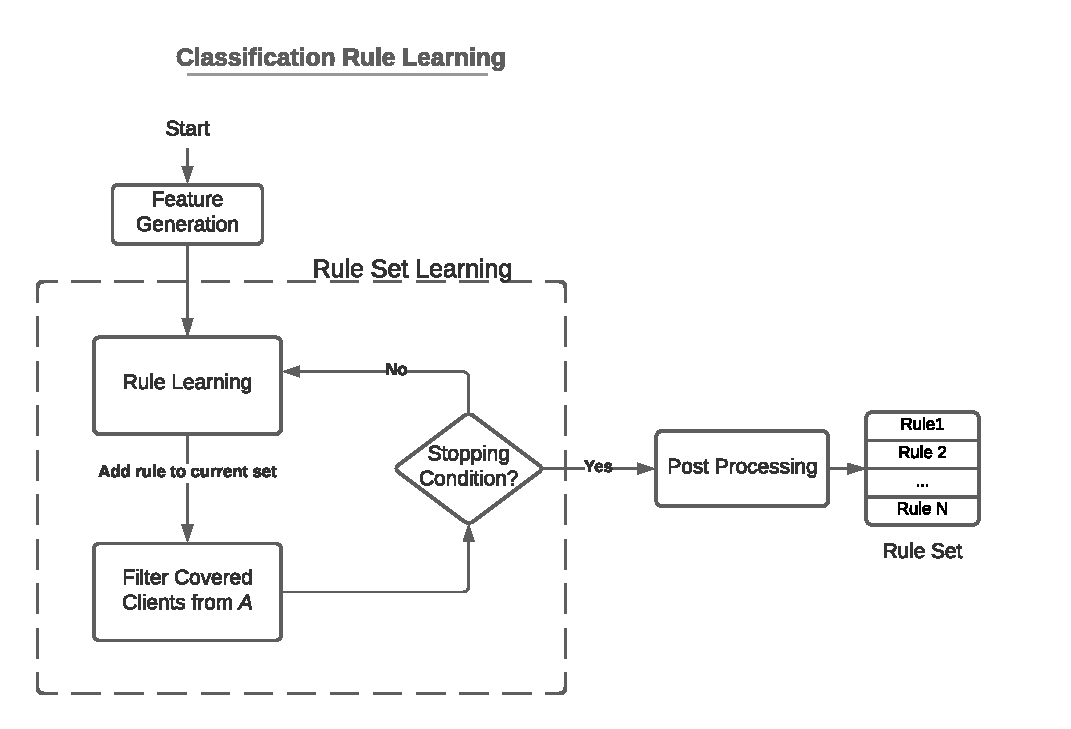
\includegraphics[width=1\textwidth]{Figures/Covering-Algorithm.pdf}
    \caption{A high-level overview of a classification rule learning system.}
		\label{fig:covering}
\end{figure}


\subsection{Feature Generation} \label{chap:rule:pre}

As features are typically descriptions of a data set (e.g Sleep $>$ 30), they will need to be derived somehow from the data. The general format of features also needs to be chosen by the system designer and will have an impact on the feature generation procedure. A common feature generation procedure is to take the range of each attribute and generate several "bins" based on this range. The bins can be evenly spaced, or the result of some clustering algorithm. The resulting "bins" will be used as features (e.g 25 $<$ Sleep $<$ 30). Another approach is to consider thresholds, which are the same as bins, but one side is unbounded (e.g. Sleep $>$ 24). More examples are provided in Table \ref{tbl:rule:examplefeatures}. Similarly, these threshold values can be evenly spaced, exponentially spaced, or based on some clustering or partitioning algorithm. 

A common problem with rule learning is that the space of all possible rules is large ($\sum_{k=1}^{|\mathcal{F}|} {|\mathcal{F}| \choose k}$), and many (if not most) rules are not useful. Due to the combinatorial nature of rules with respect to features, the complexity of the rule space increases exponentially with the number of features. The feature generation procedure needs to take this into account and generate a minimal set of features that can support high-quality rules. Additionally, this means there is much to be gained from removing features that are not useful before the learning process begins. There are many methods of determining the usefulness of a feature, but perhaps the two most common are pairwise correlation and feature coverage.

Pairwise correlation examines every available feature and builds a correlation matrix, that is, a matrix whose columns and rows are the set of all features, and whose values are the correlation between those features. The Pearson correlation coefficient \cite{benesty2009pearson} can be used to get these correlation values. A correlation threshold is then given and any pairs with a correlation higher than the threshold will be reduced to a single feature. One method of determining which feature in the pair should be removed is to take the sum of all correlations of the two features and discard the one with a larger total correlation. This pruning is then repeated on the reduced set of features until all pairs are below the given correlation threshold.

As noted above, each feature applied to $A$ generates a list of clients matching the feature. A features coverage is the number of positive individuals who match the feature (in this work, clients who are chronic or have the potential to become chronic are considered for coverage). A feature with low coverage can only produce rules with even lower coverage (as noted in Section \ref{chap:rule:back}, paragraph 1). This suggests that features with abnormally low coverage can be excluded from the rule learning procedure as they are unlikely to produce useful rules.
Another reason to trim low coverage rules is they can lead to over-fitting. Rules with low coverage are inherently over-fit as they target a small subset of the population that does not necessarily represent the broader chronic population.
In this work, low coverage is defined as having a Support $< 0.5\%$, which in this data set covers approximately 5 clients.

After this stage, the rule learning system will have a set $\mathcal{F}$ of available features. Table \ref{tbl:rule:examplefeatures} contains a list of example features using attribute names from Chapter \ref{chap:data}.


\begin{table}[h]
	\centering

	\begin{tabular}{c}
	\toprule
	Sleep $> 30$ \\
	Bar $\leq 1$ \\
	Log $= 15$ \\
	$55 \leq$ Age $< 79$ \\
	Log $> 15$  \\
	Sleep $\leq 30$ \\
	Bar $> 1$ \\
	EmployeeIsCounsellor $< 6$ \\
	Age $> 65$ \\
	CounsellorsNotes $> 16$ \\

	\bottomrule
	\end{tabular}

	\caption{Example features.}
	\label{tbl:rule:examplefeatures}
\end{table}


\subsection{Learning Individual Rules} \label{chap:rule:individual}
Within the context of rule learning, the user is often most interested in the best rule (or top $N$ rules) possible from a set of features $\mathcal{F}$. Best refers to a rule's ranking with some given quality metric. For example, a common quality metric is Accuracy, which measures the proportion of correct positive and negative classifications. See Appendix \ref{chap:perf} for an evaluation and discussion of different metrics.  Alternatively, a user might want a list of all rules sorted by some given quality metric. In both cases, a search algorithm must be employed that will discover the top rules.

In general, all of these search algorithms follow the same process. Initially, the search space is $\mathcal{F}$ and the initial rule is the default rule. The default rule being the class label that will be assigned to the examples that are not covered by the rule set. In binary classification systems such as this, the default rule has no features and results in a negative classification (not chronic in this work). Using Table \ref{tbl:rule:examplefeatures} as $\mathcal{F}$, a rule learner would begin the learning process by selecting one feature randomly (typically the first feature in the set). For example, the Sleep $> 30$ feature could be added to the current rule. The next step will be determined by the exact search algorithm used.

The simplest of these search algorithms would be breadth-first search (BFS) and depth-first search (DFS). Both of these algorithms are examples of exhaustive search and will discover all rules within a bounded search space. The only difference is the order in which rules are discovered.

BFS is an iterative algorithm that searches all rules made up of only a single feature, before searching all rules made up of two features, and so on. Continuing from the above example, the BFS algorithm will create a set of rules from Sleep $> 30$ and the remaining features in $\mathcal{F}$, (e.g. Sleep $> 30$ AND Bar $\leq 1$, Sleep $> 30$ AND Log $= 15$, etc.) producing $|\mathcal{F}| - 1$ new rules. For each rule in this resulting rule set, the above procedure will be duplicated, that is, each rule that was just added to the rule set will produce $|\mathcal{F}| -2$ new rules. This procedure is repeated until all possible rules are created from $\mathcal{F}$. The rules can now be ranked by a quality metric (e.g. Accuracy) and the best rule (or best $n$ rules) can be returned.

DFS recursively searches the space of all possible rules and adds features to the current rule until there are no more available features, or some other stopping condition is met. This is conceptually the same as BFS, but the order of rule generation is different. Starting again with one rule, Sleep $> 30$, the DFS algorithm will create the next rule by adding a feature from $\mathcal{F}$, for example, Sleep $> 30$ AND Bar $\leq 1$. The next step will add a feature to the current rule, for example, Sleep $> 30$ AND Bar $\leq 1$ AND Log $=15$. The algorithm will continue adding one feature at a time until $\mathcal{F}$ is empty, at which point it will backtrack and substitute one feature for another. For example, at one stage in the algorithm, the rule Sleep $> 30$ AND Log $= 15$ will be generated. The generated rules will be identical to the BFS algorithm, hence they are both exhaustive search techniques. The difference between these techniques becomes apparent when stopping conditions aside from $|\mathcal{F}| = 0$ are used, as this is when rule set ordering can become relevant.

It is common to use a given depth as a stopping condition, as in, only rules up to a certain depth will be created. Another common stopping condition is to supply a given rule quality measure and set a minimum value for the measure. While these simple search algorithms are quite powerful, the entire search space of all possible rules is often large enough that it can be infeasible to search beyond a depth of 2 or 3.
Along with limits on search depth, exhaustive search techniques can suffer from over-searching \cite{quinlan1995oversearching} \cite{janssen2008oversearching}. That is, the ability to search over all possible rules can result in a rule learning system that over-fits the data and will not generalize well.
 Fortunately, there are heuristics that can be used to reduce the search space and help prevent over-searching.

 The Apriori algorithm \cite{agrawal1996fast} is most famously used in the field of association rule learning, but has also been adapted for use in classification rule learning \cite{liu1998integrating} \cite{liu2000improving} \cite{jovanoski2001classification}.The Apriori algorithm is a heuristic search based on BFS. The algorithm differs from BFS by evaluating each generated rule and discarding all rules that fall below a given quality threshold. This heuristic limits the search space thus allowing for more efficient discovery of rules. The quality measures used are Support, Confidence, and Lift. These measures are precisely defined in Appendix \ref{chap:perf}, but for now, it is enough to know that Support is equivalent to the coverage of a rule, Confidence is the conditional probability of a true positive, and Lift represents the improvement of Confidence relative to a random guess.
 Confidence should not be confused with the similarly named Confidence Intervals. The definition of Confidence used in this work is alternatively called Precision, but Confidence will be used here to align with the field of association rule learning.
 If a generated rule is below the given Support it will be removed from consideration. This effectively reduces the severity of over-searching by reducing the search space of the algorithm (which removes the guarantee of a global optimum). Using Support in this way performs the same role as the coverage feature-filtering technique in Section \ref{chap:rule:pre}. After the rules have been generated, all the rules are sorted by Lift, and any rule with Lift less than 1 is removed. These are rules that do not provide additional Confidence beyond a random guess.

 Hill climbing is an alternative type of rule search algorithm, which follows a DFS approach, allowing it to discover much longer rules. The difference is that hill climbing will only follow a single path (it is not exhaustive). Hill climbing starts with the set of all features and selects the "best" feature, based on some provided quality measure. This feature is added to the current rule, and the procedure is repeated, $|\mathcal{F}|-1$ new rules are generated by adding a feature to the current rule and the "best" rule is selected. This procedure is repeated until some stopping condition is met. This condition can be the same as above (maximum depth) or something specific to hill climbing such as stopping when the quality difference between the current rule and the previous falls below a given threshold. The difference between hill climbing and DFS is hill climbing adds features based on which current feature will produce the best rule, and hill climbing never backtracks. This makes hill climbing very efficient because it does not generate all possible rules.
Unfortunately, hill climbing suffers from myopia by following the current optimal path and can thus miss a globally optimal rule that has a non-optimal predecessor.

Beam search is an improvement on hill climbing that maintains a "beam" of the $b$ best rules and will generate the set of potential rules by extending the $b$ best rules. The hill climbing procedure is simply the beam search with a beam size of $b=1$. Similarly, DFS is a beam search with $b=|\mathcal{F}|$. This alleviates the problem somewhat by allowing for an expanded search space but does not guarantee a globally optimal solution.

% This stage will generate a rule made up of one or more features. Table \ref{tbl:rule:examplerules} demonstrates a set of fabricated rules, made up of features from Table \ref{tbl:rule:examplefeatures}.


% \begin{table}[h]
% 	\centering

% 	\begin{tabular}{c}
% 	\toprule
% 	Sleep $> 30$ AND Bar $\leq 1$ \\
% 	Sleep $> 30$ AND Log $= 15$ \\
% 	Bar $\leq 1$ AND Age $> 65$ AND Sleep $\leq 30$ \\
% 	Log $> 15 10$ AND CounsellorsNotes $> 16$ \\
% 	Log $= 15$ AND Sleep $> 30$ AND Bar $> 1$ \\
% 	CounsellorsNotes $> 16$ AND EmployeeIsCounsellor $< 6$ AND Bar $\leq 1$ \\

% 	\bottomrule
% 	\end{tabular}

% 	\caption{Example rule set.}
% 	\label{tbl:rule:examplerules}
% \end{table}

\subsection{Learning Rule Sets} \label{chap:rule:sets}
Just as with rule learning, rule set learning is another simple operation that can be performed in any way that the rule learning system designer sees fit. For example, the most basic rule set learning algorithm would be to take the top $N$ rules generated by the rule learning procedure. This is not an ideal approach as it does not examine the impact each rule has on the rule set and can produce significant overlap between rules. Slightly more complex than that is the commonly used Covering algorithm \cite{michalski1969covering}.

The Covering algorithm, as the name suggests, is primarily concerned with the effect a new rule will have on the population covered by a rule set. Specifically, the covering algorithm is a loop that has two main functions. First, it searches for the top rule in the set of all rules (using any rule search method). Second, it removes all individuals covered by that rule from the attribute table. These two operations are repeated, with the rule learning procedure using the new attribute table at each iteration, and each rule learned being added to the current rule set. The loop stops when a given stopping condition is reached.
The stopping condition is typically when there are no more available rules, or when the rule set has 100\% coverage of the positive examples. This basic loop can perform fairly well but is often too eager in removing covered clients, which can impact the performance of rules generated later as they will have a much smaller database to draw from.

The weighted covering algorithm \cite{lavrac2004weighted} is a modification to the standard covering algorithm that assigns each client a weight. This weight is used by the top rule generating algorithm and corresponds to the degree a client should be considered by the rule learning procedure. Each time a client is covered by the top rule, this weight is reduced until a client is dropped entirely from consideration. The standard covering algorithm can be seen as a special case of the weighted covering algorithm, where a client is dropped from consideration after only being covered a single time. A simple method of calculating weights is the additive weighting scheme \cite{lavrac2004weighted} which is defined $weight = 1/(1+n)$ where $n$ is the number of times a client has been covered in the covering loop. The additive weighting scheme is recommended for experimental use in \cite{lavrac2004weighted}.

% After this stage, the rule learning system will have generated a rule set just like the one presented in Table \ref{tbl:rule:examplerules}. Note, there is not typically a limit to the number of rules in a rule set, the example in Table \ref{tbl:rule:examplerules} is fabricated.

\subsection{Post-Processing} \label{chap:rule:post}

The post-processing step can take place after rule set generation, or after the single rule procedure. It is used to compensate for possible over-fitting during the rule (set) learning procedure. Typically this is some form of pruning procedure (removing features from a rule). While there are several pruning procedures, such as Reduced Error Pruning \cite{brunk1991rep} or Reduced Error Regrowth \cite{cohen1993pruning}, a full examination of these methods will not take place in this work. Instead, a general introduction to the broad technique will take place.

The procedure for pruning proposed by Pagallo and Haussler \cite{pagallo1990pruning} is to split the data into a growing set $\mathcal{G}$ and a pruning set $\mathcal{H}$. These are similar to a training and testing set. The growing set $\mathcal{G}$ is used for the rule learning procedure, resulting in a set $\mathcal{R}$.
The rules in $\mathcal{R}$ then undergo the pruning process. The pruning process is a simple loop that removes one feature from one rule at a time. The rule set performance is then tested against $\mathcal{H}$ using either the same quality metric as was used in rule set learning, or a different one. If the prune successfully improves the rule set quality, it will be accepted and the pruning procedure will be repeated on $\mathcal{R}'$. The pruning procedure stops once additional prunes are unable to increase the quality of $\mathcal{R}'$. The pruning procedure is useful in combatting over-fitting by removing features that make rules overly specific (over-fit).

% Table \ref{tbl:rule:exampleprune} demonstrates a new rule set that might be generated after the rule set in Table \ref{tbl:rule:examplerules} was subjected to such a pruning procedure. Features highlighted in red are those that have been pruned by the pruner. In this (fabricated) example, the pruner has removed some redundant features and some features that did not improve the rule quality.


% \begin{table}[h]
% 	\centering

% 	\begin{tabular}{c}
% 	\toprule

% 	\prune{Sleep $> 20$ AND} Log $> 22$ \\
% 	Sleep $> 30$ AND Age $> 55$ \\
% 	\prune{Bar $\leq 1$ AND} Age $\geq 55$ AND Sleep $> 25$ \\
% 	Log $< 10$ AND CounsellorsNotes $< 5$ \\
% 	Log $< 3$ \prune{AND Sleep $> 15$} AND Bar $\geq 3$ \\
% 	CounsellorsNotes $> 16$ \prune{AND EmployeeIsCounsellor $>12$ AND Bar $\leq 1$} \\

% 	\bottomrule
% 	\end{tabular}

% 	\caption{Example rule set after pruning.}
% 	\label{tbl:rule:exampleprune}
% \end{table}

\section{RIPPER} \label{chap:rule:ripper}



\RIPPER (RIPPER) \cite{cohen1995ripper}, known by the popular JRIP, an implementation of RIPPER in the Java programming language included in the WEKA workbench \cite{frank2005jrip} is a highly regarded classification rule learning system. RIPPER was designed primarily to overcome the over-fitting issues described above and to improve the efficiency of its predecessor \IREP (IREP) \cite{frnkranz1994irep}. As such the broad structure of the RIPPER and the IREP algorithms are the same, only the RIPPER algorithm will be presented here. The reader is referred to \cite{frnkranz1994irep} for more information on IREP. The following sections will break the RIPPER algorithm into four sections of classification rule learning, feature generation, rule learning, rule set learning, and post-processing and detail each one.

\subsection{Feature Generation}
The RIPPER algorithm considers features of the form $a_n = v$ where $v$ is a value present in $a_n$ and $a_n$ is made up of integer values. For continuous attributes, RIPPER considers features of the form $a_c \leq \theta$ and $a_c \geq \theta$ where $\theta$ is a value present in attribute $a_c$.
For example, the feature Log $= 15$ from Table \ref{tbl:rule:examplefeatures} is a feature of the form $a_n = v$. The attribute matrix $A$ does not contain any continuous attributes, but a feature of this form would look like the second feature in Table \ref{tbl:rule:examplefeatures}, Bar $\leq 1$.

\subsection{Learning Rules/Learning Rule Sets}
Before rule generation, the data set is split into a growing set ($\mathcal{G}$) and a pruning set ($\mathcal{H}$).
The basic covering algorithm is employed for the rule set learning stage, and the individual rule learning is performed with a hill climbing algorithm that makes use of \FOIL's (FOIL's) \cite{quinlan1990foil} information gain metric as the quality measure.
FOIL is a relational learning algorithm that uses information gain to learn logical relations. One area that FOIL was shown to work in is a chess endgame scenario where logical predicates were used to encode legal and illegal moves \cite{quinlan1990foil}.
The RIPPER algorithm stops generating rules when the description length of the rule set plus the class label vector $C$ exceeds the previous description length by more than 64 bits. Description length is analogous to the number of bits needed to transmit the rule set (or $C$) over a communications channel, the exact definition used can be found in Cohen 1995 \cite{cohen1995ripper}. The benefit of using description length is that it gives an upper limit to the allowed complexity of a rule set.
Using the description length in bits allows a rule learner to directly compare the length of a rule set to the size of the example set ($C$).

\subsection{Post-Processing}
The final, and perhaps most distinctive step of the RIPPER algorithm is a rule optimization post-processing pass. This pass will create two modifications for each rule, the \emph{replacement} which is created by pruning the rule with the goal of optimizing the rule set on the pruning set $\mathcal{H}$. And the \emph{revision} which is formed by adding features to the rule also with the goal of optimizing the rule set (rather than optimizing the individual rules as in the first pass). These two modifications along with the original are then used in an optimization algorithm that will determine for each rule in the set which should be used.


\section{Summary}

This chapter introduced many of the fundamental concepts in rule learning. The broad architectural sections were introduced, namely feature generation/pre-processing (Section \ref{chap:rule:pre}), individual rule learning (Section \ref{chap:rule:individual}), rule set learning (Section \ref{chap:rule:sets}), and post-processing. The RIPPER algorithm was also introduced describing how it incorporates each stage. The following chapter will introduce the system proposed and implemented in this work, with motivations for each chosen stage.

 
\chapter{Rule Learning System Details} \label{chap:algo}

This chapter will introduce the proposed classification rule learning system and provide implementation details that are aligned to the goals stated in Chapter \ref{chap:intro}.
Section \ref{chap:algo:overview} gives a high-level overview of the proposed system and provides context on the broad choices made.
Section \ref{chap:algo:binning} describes the feature generation procedure used in this work.
Section \ref{chap:algo:whypriori} describes the rule learning algorithm that was chosen and why.
Section \ref{chap:algo:weightcov} describes the Weighted Covering Algorithm and why it was chosen for this system.
Section \ref{chap:algo:proposed} covers the overall system and how it is evaluated.

\section{Overview} \label{chap:algo:overview}
The proposed system is called \Name (\Abb) and has two stages of interest, one is a classification rule learning system (seen in Figure \ref{fig:covering}), and the other is a higher level covering loop that operates on rule sets (Figure \ref{fig:highlevel}). Both stages are designed to be as simple as possible to enable a transparent view into their operation. 



\begin{figure}[h]
    \centering
    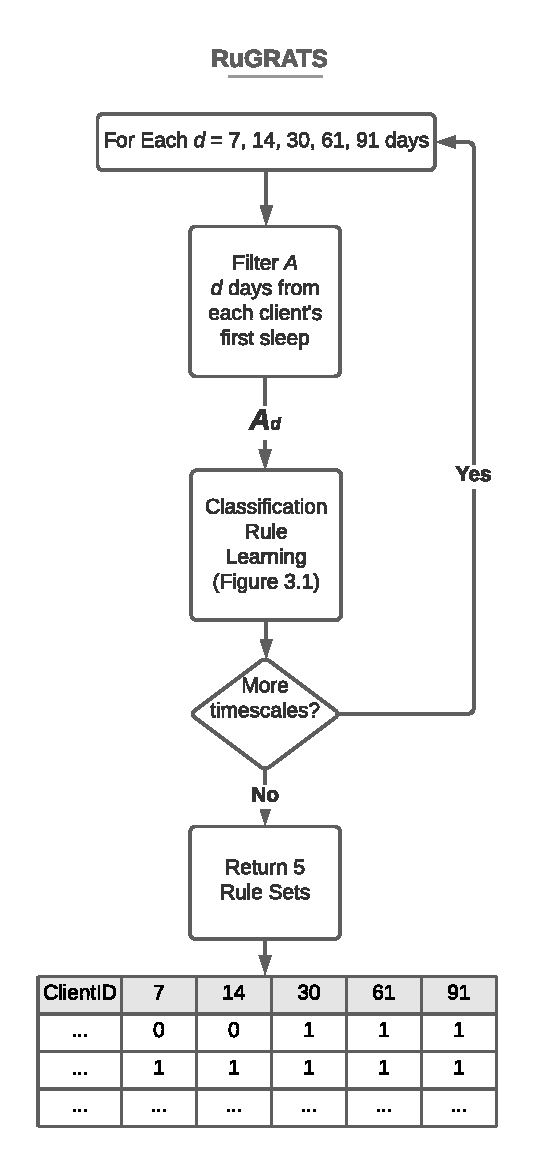
\includegraphics[width=0.5\textwidth]{Figures/RuGRATS.pdf}
    \caption{A high-level overview of the proposed algorithm structure.}
		\label{fig:highlevel}
\end{figure}

The outer stage (Figure \ref{fig:highlevel}) is proposed in this work as a means to identify potentially chronic individuals as early as possible. The general function of this loop is to extend the concept of rule sets, to \emph{time-dependent} rule sets. Which when combined allow the \Abb recommendation system to identify clients very rapidly at short time scales, while still taking advantage of the availability of data after a longer period.

Time-dependent rule sets are rule sets that are only exposed to a client's first $d$ days sleeping in shelter. Thus, the outer loop in Figure \ref{fig:highlevel} loops over a set number of time scales. In this work $d =$ 7, 14, 30, 61, and 91 days. This outer loop will generate five time-dependent rule sets, one for each value of $d$. The \Abb system will return a matrix of classifications (see Figure \ref{fig:highlevel}), with one client per row, and the columns represent after how many days the client was identified to be potentially chronic. In the figure, 0 refers to not identified, and 1 is identified. The proposed system would re-generate the matrix of classifications every day using updated data from each client. The five rule sets could also be updated daily, or updated periodically.
Section \ref{chap:algo:proposed} covers this concept in more detail and introduces a metric (Section \ref{chap:algo:mtti}) that can aid in comparing the rapidity of classification. This metric will approximate the mean identification time of a given classifier allowing multiple classifiers to be compared.

The inner stage is a typical rule set learning system (Figure \ref{fig:covering}) with a focus on simple, easy-to-understand operations. This stage employs the weighted covering algorithm (Section \ref{chap:algo:weightcov}), which repeatedly uses the Apriori algorithm to generate the top rule (Section \ref{chap:algo:whypriori}). The Apriori stage composes rules made up of features generated in the feature generation stage (Section \ref{chap:algo:binning}).
This inner stage can easily be replaced by another classification system (e.g. Logistic Regression, Neural Network etc.). Replacing the inner stage might be useful for a homeless shelter that is willing to forgo interpretability for more performant classifications. The inner stage presented here is designed to be simple with an interpretable output. As discussed in Chapter \ref{chap:intro}, classification rule learning excels in interpretability because all decision making in the classifier is encoded into a rule set.

\section{Feature Generation} \label{chap:algo:binning}

The feature format selected for this is the threshold method mentioned in Section \ref{chap:rule:pre}. Features will take the form $a < \theta$ and $a \geq \theta$ where $\theta$ is a value in the range $[1, max(a)]$ for each attribute $a$. This form was chosen carefully to avoid over-fitting and increase the fairness of classification. Features of the form $a = \theta$ will have less coverage than a rule of the form $a \geq \theta$ because they are more specific, thus leading to over-fitting. The fairness of open-ended features comes naturally from the fact that they are open-ended. For example, the feature $Sleep = 29$ will only represent clients with exactly 29 sleeps. A client with more than 29 nights in shelter would not be identified by this rule when in reality they have more nights in shelter.


The feature generation process was designed to limit the number of features generated per attribute to ten or less. As was discussed in Chapter \ref{chap:rule}, having a large number of features exponentially increases the search space of rule learning, and the time it takes to generate rule sets. The cutoff of ten features was put in place to minimize generation time, and still provide some granularity of features.
The values of $\theta$ are based on the range of attribute $a$, if $max(a) \leq 20$ then $\theta = 2n + 1 \text{ where } n \in [1, \frac{max(a)}{2} + 1]$. If $max(a) > 20$ then $\theta$ is an exponentially distributed variable with a value $\theta = \lfloor e^\frac{n\log(max(a))}{10} \rfloor \text{ where } n \in  [0, 10]$. This distribution was chosen to match the typical distribution of attributes in $A$ (shown in Figure \ref{fig:pdf}) and give features a higher resolution in the lower ranges, which represent a larger proportion of clients.
The feature reduction techniques presented in Section \ref{chap:rule:pre} are not used in this work because the above technique sufficiently reduces the number of features. The second technique presented in Section \ref{chap:rule:pre} is not needed because it is made redundant by the use of the Apriori algorithm (Section \ref{chap:algo:whypriori}).


% Table \ref{tbl:algo:examplefeatures} demonstrates some actual features used by the \Abb system. These are randomly selected features, and are specifically generated with $d=30$. For convenience, features of the form $a < 1$ are represented as 'No $a$'.

% \begin{table}[h]
% 	\centering

% 	\begin{tabular}{c}
% 	\toprule
% 	EmployeeIsCounsellor $< 3$ \\
% 	Sleep $\geq 23$ \\
% 	Age $\geq 50$ \\
% 	No Log \\

% 	\bottomrule
% 	\end{tabular}

% 	\caption{Example features.}
% 	\label{tbl:algo:examplefeatures}
% \end{table}


\section{Top Rule Learning}\label{chap:algo:whypriori}

In this work, the Apriori algorithm will be used to search for possible rules. As discussed in Chapter \ref{chap:rule}, the Apriori algorithm is very similar to the BFS exhaustive search but has the additional heuristic that it drops rules with low coverage. Dropping rules with low coverage during the search procedure reduces the search space and allows the Apriori algorithm to discover rules more efficiently. As rule length increases, rule coverage goes down (discussed in Section \ref{chap:rule:pre}), this means that dropping low coverage rules early on in the search procedure will not preclude further high-quality rules from being generated. 

The reason for using a heuristic based on exhaustive search is to combat the myopia present in hill search and beam search techniques. These algorithms do not search the entire space of possible rules and thus can get stuck in local maxima and will be unable to find the best rule. The typical reason to implement hill climbing or beam search is to discover rules with a larger depth.

Rules with a larger depth are "specific", this is in contrast to shorter rules which are "general". The terms specific and general refer to the implied coverage of a rule. That is, a rule with a large depth will have many features, with each added feature reducing the coverage, meaning that longer rules will typically have lower coverage than a similar short rule. Short rules cover general populations, for example, Sleep $>30$ is more general than Sleep $> 30$ AND Log $< 15$ because it describes a more generic population. Rules with a larger depth are therefore at risk of over-fitting. In this work, a rule depth limit of 2 is employed. This limit is in place to prevent over-fitting (and focus on more general rules), but the exact value was chosen based on computing constraints (going to a depth of 3 required 50x the computing time). An implemented system would not have the computing time constraint and could use a slightly larger depth.

% 20:35:52.269123
% vs.
% 0:24:21.123328

% 2. Exhaustive search techniques are easy to explain to the layperson user of the system. Other search heuristics, such as hill climbing and beam search require specific knowledge about searching to understand. By contrast, an explanation of the Apriori algorithm can be truthfully simplified as "All possible rules are generated, and the top rule that covers at least N clients is selected". This hides some implementation details of the Apriori algorithm, but still reflects what is happening and the intuition that a user develops will be true. Hill climbing and beam search can not be simplified in such a way, and if the above explanation is used, these techniques could return rules that do not intuitively make sense to a shelter operator (in the worst case of both algorithms, the local maxima is followed until a non-optimal solution is found).



Traditionally the Apriori algorithm uses the Precision measure to rank rules. For this work, other measures were considered with the goal of improving classification performance. Appendix \ref{chap:perf} compares six different performance measures in the context of this work. Ultimately, the Apriori measures, Support, Precision (Confidence), and Lift were not replaced because of their tolerance to data sets with class imbalance and the intuitive nature of the rules (e.g. for Lift any value above 1 is better than a random guess).

% \tdo{How can I integrate this table?}
% Table \ref{tbl:algo:examplerules} demonstrates an example rule set made up of rules that have been generated using this procedure. Again, these rules were generated with $d=30$.

% \begin{table}[h]
% 	\centering

% 	\begin{tabular}{c}
% 	\toprule
% 	Age $\geq 50$ AND Sleep $\geq 29$ \\
% 	No Log AND Sleep $\geq 29$ \\
% 	Age $\geq 50$ AND Sleep $\geq 25$ \\
% 	Age $\geq 42$ AND Sleep $\geq 27$ \\
% 	EmployeeIsCounsellor $< 3$ AND Sleep $\geq 27$ \\
% 	Age $\geq 42$ AND Sleep $\geq 21$ \\

% 	\bottomrule
% 	\end{tabular}

% 	\caption{Example rule set.}
% 	\label{tbl:algo:examplerules}
% \end{table}

\section{Rule Set Learning}\label{chap:algo:weightcov}

The standard for rule learning is to use some variant of the covering algorithm. This work is no different and employs the weighted covering algorithm to generate rule sets. This choice was made to increase the redundancy of the generated rule sets.
The redundancy of the weighted covering algorithm allows a client to be covered $k$ times before being removed from consideration. This redundancy can help reduce the problem of over-fitting. In this work $k$ was chosen to be 5, this variable is available to be optimized but was not in this work. Following the recommendation in \cite{lavrac2004weighted}, the additive weighting scheme was used. A factor in the decision for using this scheme is the simplicity and the goal of maintaining simplicity wherever possible.

The use of the weighted covering algorithm necessitates that the implementation of Support, Precision, and Lift must take the weight of each client into account. Let $P(R)$ be the probability that a given rule classifies a client as chronic, $P(C)$ is the probability that a client actually is chronic, and $P(R \cap C)$ is the probability that a client is chronic and identified as such. $P(R) = \frac{n(R)}{N}$, $P(C) = \frac{n(c)}{N}$, and $P(R \cap C) = \frac{n(R \cdot C)}{N}$ where $n(R)$ is the number of clients identified by a given rule, $n(C)$ is the number of chronic clients, $n(R \cdot C)$ is the number of clients that are chronic and identified as such, and $N$ is the total number of clients, this follows the convention in \cite{lavrac2004weighted}. The definitions of Support, Precision, and Lift are $P(R \cap C) = \frac{n(R \cdot C)}{N}$, $P(C|R) = \frac{n(R \cdot C)}{n(R)}$, and $\frac{P(C|R)}{P(C)} = \frac{n(R \cdot C) \cdot N}{n(R) \cdot n(C)}$ respectively. In order to take weight into account, $n(R)$, $n(C)$, $n(R \cdot C)$, and $N$ will be substituted with $n'(R)$, $n'(C)$, $n'(R \cdot C)$, and $N'$. Where $N'$ is the summation of all clients weights and $n'(R)$, $n'(C)$, and $n'(R \cdot C)$ are the summation of weights of clients identified by a rule, chronic clients, and both respectively. The new definitions for Support, Precision, and Lift are $P(R \cap C) \to \frac{n'(R \cdot C)}{N'}$, $P(C|R) \to \frac{n'(R \cdot C)}{n'(R)}$, and $\frac{P(C|R)}{P(C)} \to \frac{n'(R \cdot C) \cdot N'}{n'(R) \cdot n'(C)}$ respectively.


Section \ref{chap:rule:sets} introduced the most basic stopping condition, 100\% coverage. In the \Abb system one more stopping condition is used, the minimum lift condition. A rule with a Lift of 1 has the same Precision as a random guess. Thus, if the top rule has a Lift of 1 or less, the covering algorithm can safely quit (there are no more good rules). In this work, the minimum lift is configurable and will be used by the outer loop to adjust the Precision of the resulting rule set. Precision measures the probability that a client becomes chronic given that they were classified as such. The Precision of a random guess in this data set is 4.82\% (the proportion of chronic clients) and any rule set Precision higher than that can be considered "good". Lift measures the improvement of Precision over a random guess, in this work, Lift is defined as $\frac{\text{Precision}}{4.82\%}$. A higher minimum lift will increase the overall Precision of a rule set by limiting rules with low Precision/Lift.
However, a user of the system may want much more than 4.82\% Precision in decision making. Moreover, as Precision increases, coverage tends to decrease. That is, increasing the Minimum Lift Threshold will reduce the number of clients identified as chronic, but the correct proportion of identified clients will be higher. This is useful for shelter operators, as it will allow them to increase and decrease the number of identified clients based on the available resources at the time.

The rule sets presented in Table \ref{tbl:algo:exampleminlift} were generated using this procedure. Specifically, they were generated using a Minimum Lift Threshold of 2.5 and 10.6. One thing that is evident by observing this example rule set is that the Sleep attribute seems to be the most important attribute making a chronic classification. This is understandable, as the definition used to generate the chronic labels (the DI definition, Section \ref{chap:data:labelling}) is purely based on the amount of sleep. Beyond that, it is worth noting that features based on the same attribute (e.g. Sleep $\geq 25$ and Sleep $\geq 27$) are not allowed in the same rule, but are allowed in the same rule set.

As the Minimum Lift Threshold is an early stopping condition it will affect the number of rules in a generated rule set. Table \ref{tbl:algo:exampleminlift} demonstrates this with two rule sets with a Minimum Lift Threshold of 2.5 and 10.6. As can be seen, the higher Minimum Lift Threshold significantly reduces the length of the generated rule set. These rule sets are selected examples that were generated as part of the results in Chapter \ref{chap:results}.

\begin{table}[h]
	\centering

	\begin{tabular}{cc}
	\toprule
	2.5 & 10.6 \\
	\midrule
	Age $\geq 59$ AND Sleep $\geq 27$ & Age $\geq 59$ AND Sleep $\geq 27$ \\
	Age $\geq 50$ AND Sleep $\geq 29$ & \\
	No Log AND Sleep $\geq 29$ & \\
	Age $\geq 42$ AND Sleep $\geq 25$ & \\
	EmployeeIsCounsellor $< 3$ AND Sleep $\geq 27$ & \\
	Age $\geq 50$ AND Sleep $\geq 21$ & \\
	\bottomrule
	\end{tabular}

	\caption{Example rule sets generated with Minimum Lift Thresholds of 2.5 and 10.6.}
	\label{tbl:algo:exampleminlift}
\end{table}


\section{Outer Covering Loop} \label{chap:algo:proposed}


The \Abb system proposes an outer covering loop to minimize the amount of time before a chronic classification can take place. To do this, multiple rule sets are generated where each rule set is generated using a modified attribute table with a different number of days $d$. This work uses $d$ values of 7, 14, 30, 61, and 91. These values can likely be optimized, but in the interest of simplicity, these are suitable for experimental demonstration. If this system were to be deployed, alternative values would be investigated. 

The generation process of \Abb is simply repeated generation of rule sets with the different values of $d$. If a single rule set were used the user or system designer would be presented with a trade-off. A small value of $d$ results in more rapid classification time, but lower coverage and potentially lower Precision. A large value of $d$ has better coverage and potentially better Precision, but suffers from the longer classification time. This work removes that trade-off by generating multiple rule sets. 


However, removing this trade-off does not come free. The system designer (or user) is now responsible for determining the minimum lift condition for each of the five rule sets generated in the \Abb system (as opposed to just one). In this work, three methods for determining these values are proposed. The first is the Lazy approach, this approach has the user set a minimum lift value for all rule sets. The second is the Greedy approach which selects minimum lift values that maximize the Precision for each rule set. These values are chosen by sweeping the Minimum Lift Threshold and selecting the value that maximizes the rule set Precision.
The rule sets generated by the Lazy system will tend to be longer than those generated by the Greedy system because the Minimum Lift Threshold will tend to be lower.
Thus the Greedy system will identify fewer clients than the Lazy system, but the identified clients have a higher probability of being chronic. The third approach is to leave setting the Minimum Lift Threshold values up to the user. This approach is, of course, difficult to evaluate in advance but allows a user to best tailor the system to the current needs of a shelter and its clients. Chapter \ref{chap:results} will evaluate the Lazy and Greedy methods.


Using the \Abb system to generate predictions is much the same as using a single rule set. The difference is that the order of evaluations will need to be considered. That is, in this work, five different time scales are used, meaning five different lists of clients will be identified as at risk to become chronic. The user of the system will need to manually determine the prioritization of clients across these lists. This is considered a benefit as it allows the system to mesh with shelter operations and allows a human to have the final say on critical decisions such as housing. This is particularly important for shelter operators because it will allow them to limit the number of False Positives when housing resources are scarce and it allows them to identify more clients when housing resources are available.

An effect of generating rule sets using different time scales is that the generated rule sets will have a different number of rules and likely a different diversity of rules. Table \ref{tbl:algo:exampledays} demonstrates this with two rule sets, one generated with $d=7$ and the other with $d=91$. As can be expected the rules in the rule set with $d=91$ are much richer, this is because there is more client data available after 91 days. A note, some rules are redundant, particularly in the $d=7$ rule set, and could be automatically removed to make the rule set more clear. This is not shown here but should be employed if this system is used. A typical cleaning method is the pruning operation discussed in Chapter \ref{chap:rule}. Another option is to simply numerically compare the overlap of the rules. For example, the $d=7$ rule set in Table \ref{tbl:algo:exampledays} can be reduced by observing that the features are the same in all rules and can be combined by taking the minimum value of each feature. Thus, the $d=7$ rule set can be reduced to the single rule Age $\geq 42$ AND Sleep $\geq 5$.

\begin{table}[h]
	\centering

	\begin{tabular}{cc}
	\toprule
	$d=7$ & $d=91$ \\
	\midrule
	Age $\geq 59$ AND Sleep $\geq 7$ & Age $\geq 42$ AND Sleep $\geq 91$ \\
	Age $\geq 50$ AND Sleep $\geq 7$ & Age $\geq 59$ AND Sleep $\geq 55$ \\
	Age $\geq 42$ AND Sleep $\geq 7$ & No EmployeeIsCounsellor AND Sleep $\geq 55$ \\
	Age $\geq 50$ AND Sleep $\geq 5$ & Age $\geq 50$ AND Sleep $\geq 55$ \\
																	 & Age $\geq 42$ AND Sleep $\geq 55$ \\
																	 & Log $< 4$ AND Sleep $\geq 55$ \\
																	 & Age $\geq 50$ AND Sleep $\geq 33$ \\

	\bottomrule
	\end{tabular}

	\caption{Example rule sets generated with different time scales, $d=7$ and $d=91$.}
	\label{tbl:algo:exampledays}
\end{table}

\subsection{Mean Time to Identification} \label{chap:algo:mtti}

The purpose of the \Abb system is to identify potentially chronic individuals as rapidly as possible. Ideally, there would be a method to measure and compare the timeliness of classification. In this work the Mean Time To Identification (MTTI) measure is proposed to do exactly this. MTTI is calculated using a loop similar to the covering algorithm, that is, the rule sets are applied to the data set one at a time starting with the smallest value of $d$. For each rule set, the number of covered chronic clients is recorded and those clients are removed from the data set. This procedure is repeated until all the rule sets have been used.
The mean of each classification time ($d$) is then taken, chronic clients who are not identified by one of the five rule sets are assumed to be classified using the DI definition (Section \ref{chap:data:labelling}). A result of using mean identification time, rather than median is that the mean identification time will be able to represent clients who are identified by the classifier and those that are not (true positives and false negatives). Having a small MTTI value is thus reflective of a classifier being able to identify a large number of individuals, and being able to identify them in shorter time scales. Chapter \ref{chap:results} will make use of this measure to compare \Abb strategies.

% Geoff commented on my second assumption asking if it was necessary.
% I feel it's necessary because in the case of some episodic clients, they are 
% "Successfully housed" but still experience episodes of homelessness afterwards
The MTTI measure does not measure the time that a client will be homeless, and does not provide any sort of guarantee as to the identification time for a specific client.
This is because MTTI makes three key assumptions. The first assumption is that clients that are identified and immediately housed after $d$ days for each rule set (e.g. the assumption is that all clients identified in the $d=7$ rule set are identified after 7 days). This assumption is false because it assumes that every client is immediately housed and does not allow for delays.
The second assumption is that clients who are identified by the system never re-enter homelessness. The assumption is not true because clients often experience multiple episodes of homelessness.
The third assumption is that clients who are not identified by the classification system will be identified after 666 days (the mean time to identification for the DI definition, Section \ref{chap:data:labelling}). This assumption is false because it only uses the mean identification time for the DI definition and does not take the distribution of identification time into account. For example, Table \ref{tbl:stats:chronic} demonstrates that the minimum time to chronic identification is 276 days, and Section \ref{chap:data:labelling} shows that the median is 349 days.
So the MTTI measure is not a completely accurate measure of identification speed. Instead, the MTTI measure provides a simple metric to compare different classification systems based on the \Abb system.


\section{Summary}

This chapter introduced the details of the \Name (\Abb) system. The feature generation, top rule learning, and rule set learning procedures were more concretely discussed and solidified. Across all stages of this system, simplicity was preferred to allow users to understand the procedures. This also extends to the outer loop of the \Abb system that functions primarily to give users insight into clients who are at risk of becoming chronic. The following chapter (Chapter \ref{chap:results}) will evaluate the \Abb system along with the \Abb rule set learning algorithm and compare it against more commonly used classification systems.


 \chapter{Results} \label{chap:results}

To get an understanding of how the \Abb recommendation system performs relative to other techniques, the results will be presented in two sections. Section \ref{chap:results:sets} will compare the rule set learning system proposed in Chapter \ref{chap:algo} to Logistic Regression and Decision Trees. Section \ref{chap:results:rapid} will evaluate the \Abb system using the Lazy/Greedy approaches as well as using a \Abb system based on Linear Regression.


\section{Rule Set Performance}\label{chap:results:sets}

The rule set learning procedure from the \Abb system will be compared against Logistic Regression  \cite{hastie2009elements} and Decision Trees \cite{chen2016xgboost}. These techniques were briefly introduced in Chapter \ref{chap:intro} and \ref{chap:rl}. As mentioned in Section \ref{chap:algo:overview}, the \Abb system could make use of any machine learning system. This makes it important to directly compare the proposed inner rule set learner to other techniques.
Logistic Regression was chosen due to its prevalence in social and medical fields \cite{allegheny2019homeless} \cite{hong2018applications} \cite{toros2019early} and inherent interpretability.
Decision trees were chosen because of their similarity to classification rules. Decision Trees can be represented as rules, making them equally interpretable. The XGBoost library \cite{chen2016xgboost} was chosen to implement the Decision Trees. The XGBoost also supports Random Forests, which are an extension of Decision Trees (detailed in Chapter \ref{chap:rl}) that typically increase classifier performance. Using Random Forests from the XGBoost library is just as easy as using Decision Trees, so the below results will include a comparison to both Decision Trees and Random Forests.

Results will be presented with the confusion values first (True Positives, False Positives, True Negatives, and False Negatives). It is the author's preference to show these values as they present the full picture of classifier quality (and any quality metric can be derived from these four values, see Appendix \ref{chap:perf}). Confidence, Sensitivity, and Specificity will also be presented for convenience. In general, the Confidence and Sensitivity metrics will also be discussed as they neatly combine the confusion values and allow for the text to be more expressive.


\subsection{Baseline Algorithm Parameters}
The \Abb system generates rule sets based on multiple different time scales (values of $d$). However, this section will only compare the rule set learning used in \Abb, meaning only a single time scale can be used. In this section all three systems will be trained on and evaluated on a time scale of 30 days, that is, only a client's first 30 days since sleeping at the DI will be used. 
The rule set learning system of \Abb will use all the parameters discussed in Chapter \ref{chap:algo}.

All presented results are the averaged values from using 10-fold stratified cross-validation. 
The Logistic Regression was performed using the scikit-learn \footnote{scikit-learn version 0.20.3 obtained via pip} library implementation of Logistic Regression. As noted above XGBoost \footnote{XGBoost version 1.02 obtained via pip} was used for the Decision Tree and Random Forests implementations. In general, the default or recommended values were used for these systems, but for completeness Tables \ref{tbl:results:lrparam} and \ref{tbl:results:xgbparam} include all parameters used.

\begin{table}[h]
	\centering

	\begin{tabular}{lr}
	\toprule
	{Name} &    Value \\
	\midrule
	Solver & 'lbfgs' \\
	Max iterations & 1000 \\
	\bottomrule
	\end{tabular}

	\caption{Parameters used for the Logistic Regression model.}
	\label{tbl:results:lrparam}
\end{table}

\begin{table}[h]
	\centering

	\begin{tabular}{lr}
	\toprule
	{Name} &    Value \\
	\midrule
	max\_depth & 2, 5 \\
	objective & 'binary:logistic' \\
	\midrule
	colsample\_bynode & 0.8 \\
	learning\_rate & 1 \\
	num\_parallel\_tree & 100 \\
	subsample & 0.8 \\
	\bottomrule
	\end{tabular}

	\caption{Parameters used for the XGBoost Decision Trees and Random Forests. Values below the midline are specific to Random Forests.}
	\label{tbl:results:xgbparam}
\end{table}


\subsection{Minimum Lift Threshold} \label{chap:results:mlt}
As discussed in Section \ref{chap:algo:whypriori}, the Minimum Lift Threshold is a parameter of the rule set learning used by the \Abb system that allows the system designer to enforce a minimum Lift value for a rule set. Also discussed was the trade-off this imposes between rule set Confidence and coverage (Sensitivity).
Figure \ref{fig:conf-sweep} displays this trade-off between Confidence and Sensitivity by sweeping the Minimum Lift Threshold from 0.5 to the maximum possible lift value of 21 with 50 steps.
As can be seen, the Confidence can only increase so far before the system fails to find rules that surpass the Minimum Lift Threshold. The reason that Confidence moves in almost direct proportion to the Minimum Lift Threshold is that the Minimum Lift Threshold restricts the quality of rules that are added to the rule set. Thus, increasing the Minimum Lift Threshold will increase the Confidence of the rule set. The corollary is that there will be fewer rules in the rule set, which will reduce the Sensitivity, as discussed in Section \ref{chap:rule:back}.
This relationship can be valuable for \Abb users because it will allow them to increase the Minimum Lift Threshold when high-quality rules that only identify a few individuals are desired. Conversely, it will allow the user to lower the threshold when they are willing to accept a lower Confidence and desire a higher Sensitivity.


\begin{figure}[ht]
    \centering
    \figuretitle{Minimum Lift Threshold Sweep}
    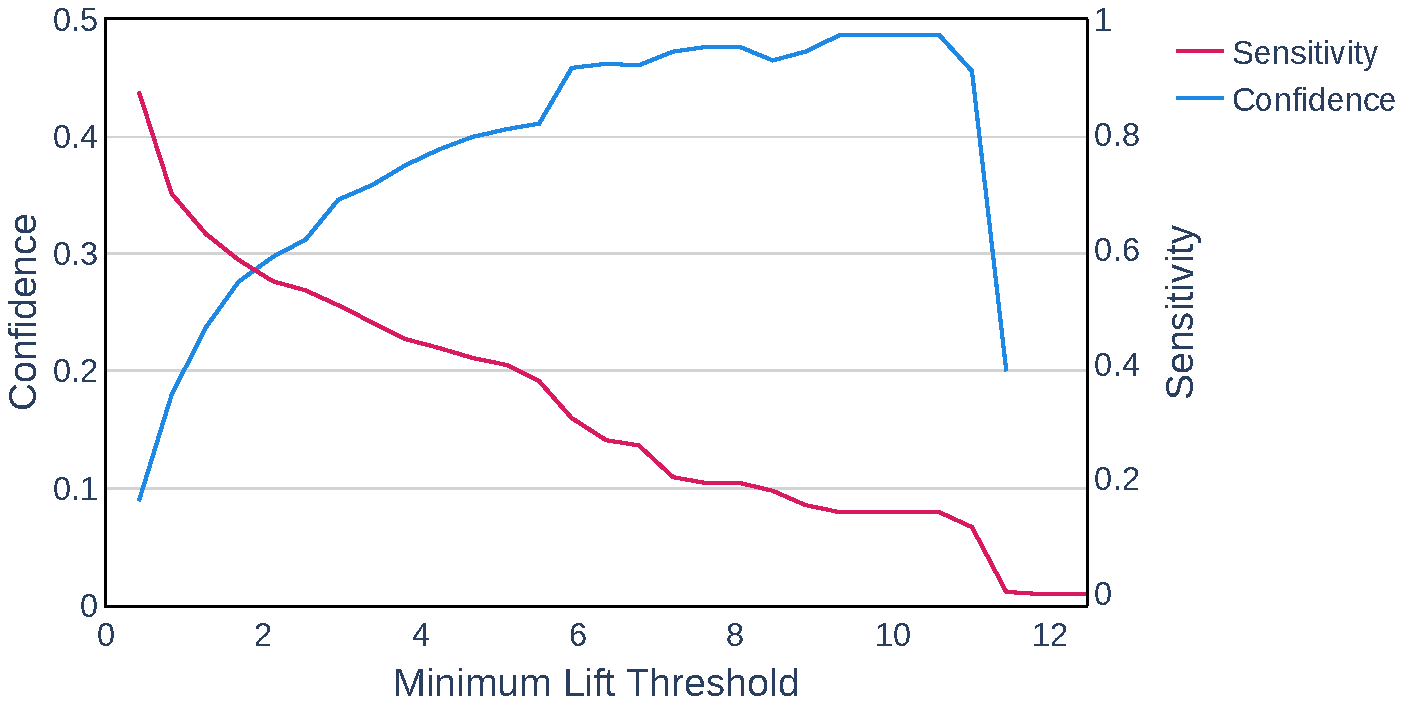
\includegraphics[width=1\textwidth]{Figures/Lift-Sweep.pdf}
		\caption{Demonstration of Confidence and Sensitivity vs. Minimum Lift Threshold.}
    \label{fig:conf-sweep}
\end{figure}

\subsection{Results}


Table \ref{tbl:results:30} demonstrates the confusion values (with abbreviated column names) for the \Abb rule set learning system, Logistic Regression, Decision Trees, and the Random Forests model. 
There are three versions of the rule set learner presented here, each one with a different Minimum Lift Threshold (2.5, 6.4, 10.6). The values were chosen to roughly correspond to high, medium and low Confidence based on Figure \ref{fig:conf-sweep}.
The exactness of the values used is a result of sweep analysis in Figure \ref{fig:conf-sweep}. That is, the sweep analysis used an even step on the Minimum Lift Threshold between values of 0.5 and 21, and the three Minimum Lift values were taken from those samples.
As can be seen in Table \ref{tbl:results:30}, increasing the Minimum Lift Threshold reduces the number of True Positives (and False Positives), but at the same time increases the Confidence of the generated rule set. Thus, increasing the Minimum Lift Threshold presents a direct Confidence/Sensitivity trade-off, as discussed in Section \ref{chap:results:mlt}.

Looking below at the other algorithms, it can be seen that the Logistic Regression performs similarly to the rule set learner with a Minimum Lift of 10.6 (outperforming slightly in both Confidence and Sensitivity). The Random Forests (both depths) perform similarly to the rule set learner with a Minimum Lift of 2.5 (underperforming on Confidence but outperforming on Sensitivity).
Logistic Regression outperforms the rule set learner with Minimum lift = 10.6 in both Confidence and Sensitivity. This suggests that using Logistic Regression instead of an Apriori-based rule set learning could be beneficial especially when working in an environment where the Logistic Regression is understood. Section \ref{chap:results:rapid} includes a comparison of the \Abb system with an Apriori-based rule set learner, as well as one that uses Logistic Regression.

The Decision Trees and Random Forests classification results are presented in two variants, one with a maximum depth of 2, and one with a maximum depth of 5. This is done because the \Abb results are presented with a maximum depth of 2, but the Decision Tree/Random Forests models are capable of going to a larger depth within a reasonable amount of time. Table \ref{tbl:results:30} demonstrates that the increase in depth does not necessarily improve performance, as mentioned in Section \ref{chap:rl:tree}. As noted above, the Random Forests classifier does outperform the Decision Trees alone, however, neither classifier matches the Confidence of the \Abb rule set learner or Logistic Regression.

As seen in Table \ref{tbl:results:30}, the performance of other classifiers can be roughly approximated with the \Abb rule set learner. Additionally, the performance trade-offs (Confidence vs. Sensitivity) can be explicitly set. This is compared to using classifiers such as Logistic Regression that have an implicit trade-off. This is a tool that will be useful for users of the full \Abb system, as it can allow adjusting the Sensitivity in each time scale, thus allowing for more fine-grained control of which clients are identified. It is technically possible to adjust the Confidence/Sensitivity of Logistic Regression and Tree based models, but that was not done here. The Logistic Regression and Tree based models all use the default training procedures according to their implementation.

\begin{table}[h]
	\centering

	\begin{tabular}{p{0.3\textwidth}rrrrrrr}
	\toprule
	{Algorithm} &    TP &     FP &      TN &    FN &  Confidence &  Sensitivity &  Specificity \\
	\midrule
	\Abb rule set learner (Minimum lift = 2.5) & 468 & 1032 & 16480 & 418 & 0.3120 & 0.5282 & 0.9411 \\
	\Abb rule set learner (Minimum lift = 6.4) & 237 & 276 & 17236 & 649 & 0.4620 & 0.2675 & 0.9842 \\
	% \Abb (0.224) & 364 & 547 & 16965 & 522 & 0.3996 & 0.4108 & 0.9688 \\
	\Abb rule set learner (Minimum lift = 10.6) & 126 & 133 & 17379 & 760 & 0.4865 & 0.1422 & 0.9924 \\
	Logistic Regression & 137 & 104 & 17408 & 749 & 0.5685 & 0.1546 & 0.9941 \\
	Decision Trees (Max depth = 2) & 541 & 1528 & 15984 & 345 & 0.2615 & 0.6106 & 0.9127 \\
	Decision Trees (Max depth = 5) & 536 & 1548 & 15964 & 350 & 0.2572 & 0.6050 & 0.9116 \\
	Random Forests (Max depth = 2) & 502 & 1139 & 16373 & 384 & 0.3059 & 0.5666 & 0.9350 \\
	Random Forests (Max depth = 5) & 504 & 1302 & 16210 & 382 & 0.2791 & 0.5688 & 0.9257 \\

	\bottomrule
	\end{tabular}

	\caption{Confusion values of the \Abb rule set learner, Logistic Regression, Decision Trees, and Random Forests.}
	\label{tbl:results:30}
\end{table}


\section{\Abb Performance} \label{chap:results:rapid}
As discussed in Chapter \ref{chap:algo} the Greedy and Lazy systems will be evaluated. The system that uses Logistic Regression in place of rule set learning will also be evaluated. This will be done by first showing the confusion values for each step as well as the summarized system performance. Then the MTTI values for each system will be compared against the DI definition from Chapter \ref{chap:data}.


\subsection{Greedy}
As discussed in Chapter \ref{chap:algo}, the Greedy system uses a different Minimum Lift Threshold for each time scale. Table \ref{tbl:results:mltgreedy} shows these Minimum Lift values. They were calculated by sweeping the Minimum Lift Threshold (see Figure \ref{fig:conf-sweep} for a visualisation) for each time scale and selecting the value that maximized the Confidence of each rule set. As can be seen, as the value of $d$ increases the Minimum Lift Threshold increases as well. This is because as clients are in shelter longer, there is more data available to generate features, thus the rule set learner has a larger set of rules to pull from and can continue to generate rules even as the Minimum Lift Threshold gets large.

To get a rule set for each $d$, ten rule sets are generated using 10-fold stratified cross-validation. In most cases, the cross-validation procedure generates the same rule set 10 times, but in the case that more than one is generated, the single rule set generated the most times is selected for use. It is important to have a single generated rule set, because it will be used later in Section \ref{chap:results:rugresults}.

The rule sets used for the Greedy System are in Table \ref{tbl:results:greedysets}. Notably, none of the rule sets are made up of more than a single rule. This is because the Greedy system uses rule sets generated with the maximum possible Confidence, that is, the Minimum Lift Threshold is increased until the rule set learning only returns the top rule. The introspection of a rule set, like the one in Table \ref{tbl:results:greedysets} is one of the primary benefits of using a rule learning system. That is, the rule set can be observed and analyzed after generation.
Table \ref{tbl:results:greedysets} demonstrates that at smaller time scales, Sleep and Age are the most important features. Larger time scales however show that Age becomes less important and exposure (or lack thereof) to DI counsellors becomes an important feature. These rule sets are thus useful to understand how classification decisions are made, but they also provide a tool that shelter staff can use to understand the features of a chronically homeless person.

\begin{table}[h]
	\centering

	\begin{tabular}{lr}
	\toprule
	{$d$} &  Minimum Lift \\
	\midrule
	7     & 6.4 \\
	14    & 7.2 \\
	30    & 9.3 \\
	61    & 9.3 \\
	91    & 10.2 \\

	\bottomrule
	\end{tabular}

	\caption{Minimum Lift Threshold values for the greedy system.}
	\label{tbl:results:mltgreedy}
\end{table}


\begin{table}[h]
	\centering

	\begin{tabular}{cc}
	\toprule
	$d$ & Rule Set \\
	\midrule
	7	& Age $\geq 59$ AND Sleep $\geq 7$ \\
	\midrule
	14	& Age $\geq 59$ AND Sleep $\geq 13$ \\
	\midrule
	30	& Age $\geq 59$ AND Sleep $\geq 27$ \\
	\midrule
	61	& EmployeeIsCounsellor $< 4$ AND Sleep $\geq 61$ \\
	\midrule
	91	& EmployeeIsCounsellor $< 6$ AND Sleep $\geq 91$ \\

	\bottomrule
	\end{tabular}

	\caption{The rule sets used in the Greedy System.}
	\label{tbl:results:greedysets}
\end{table}

% \begin{figure}[ht]
%     \centering
%     \figuretitle{Maximum Confidences}
%     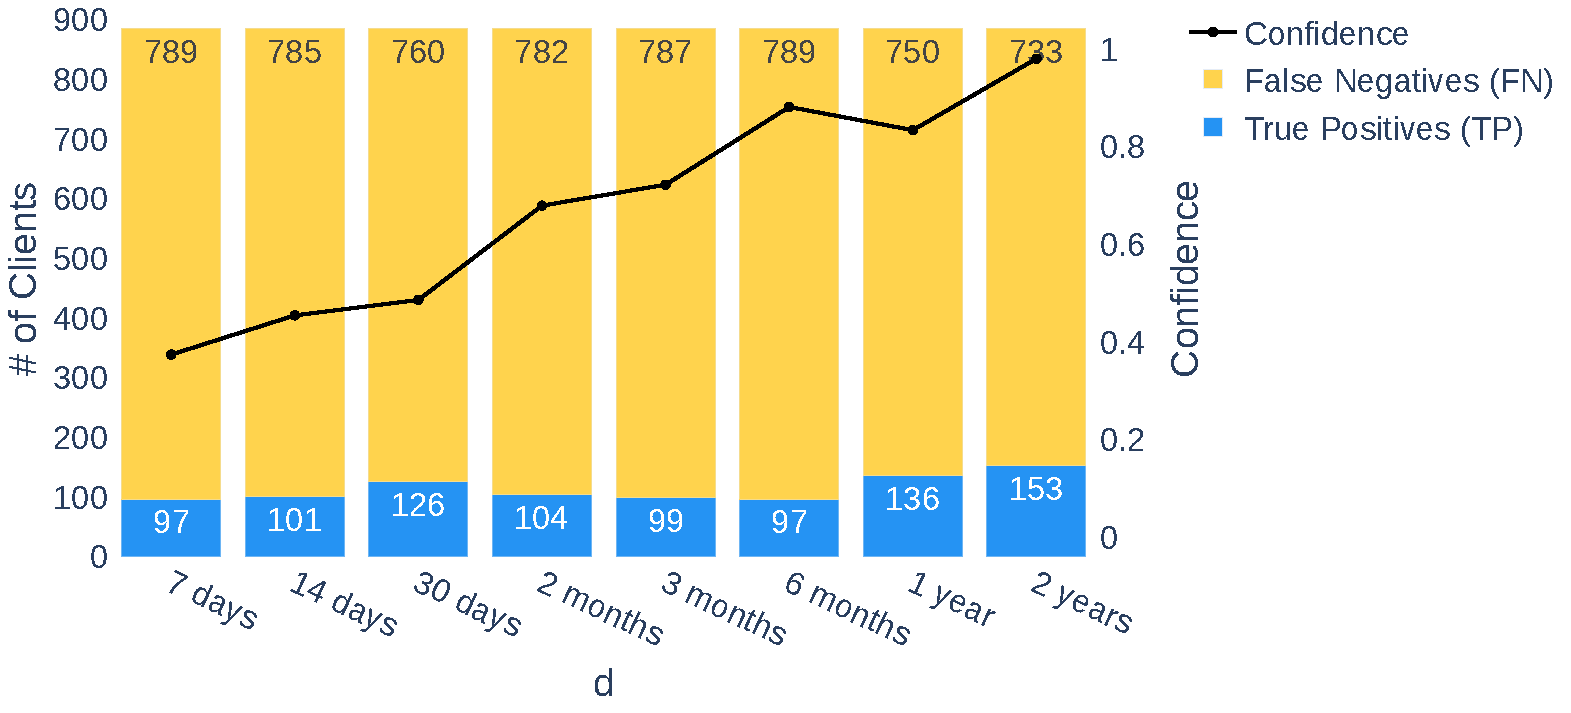
\includegraphics[width=1\textwidth]{Figures/Greedy-Columns.pdf}
% 		\caption{Confidence values taken from the rule set that maximizes Confidence at each time scale.}
%     \label{fig:greedycol}
% \end{figure}


\subsection{Lazy}

The Lazy system as introduced in Chapter \ref{chap:algo} uses a single Minimum Lift for all generated rule sets. For these results, a Minimum Lift of 6.4 is selected because it has a somewhat even trade-off between Confidence and Sensitivity (Figure \ref{fig:conf-sweep} and Table \ref{tbl:results:30}). The rule set generation procedure is the same as used in the Greedy system.

Table \ref{tbl:results:lazysets} shows the rule sets used in the Lazy system. The most notable difference to the Greedy system is that the last three rule sets in the Lazy system have more than a single rule. The first two rule sets are the same in the Lazy and Greedy systems. This is because the first two Minimum Lift values used in the Greedy system are very close to the 6.4 used in the Lazy system (6.4 and 7.2, Table \ref{tbl:results:mltgreedy}). The last three rule sets all start with the same rule as the Greedy system, this is due to the behaviour of the Covering loop detailed in section \ref{chap:algo:weightcov}. Namely, that the rules are added to the rule set in order of highest Lift to lowest.

Some insights into the characteristics of chronic homelessness can be drawn from Table \ref{tbl:results:lazysets}. In particular, the importance of Sleep events on a chronic identification are very apparent. Another important observation is that individuals who have not met with a DI counsellor (or have few meetings) are more likely to become chronic. A different way of looking at this is that clients who have regular meetings with counsellors are more likely to become housed.

\begin{table}[h]
	\centering

	\begin{tabular}{cc}
	\toprule
	$d$ & Rule Set \\
	\midrule
	7 	& Age $\geq 59$ AND Sleep $\geq 7$ \\
	\midrule
	14	& Age $\geq 59$ AND Sleep $\geq 13$ \\
	\midrule
	30	& Age $\geq 59$ AND Sleep $\geq 27$ \\ 
			& No EmployeeIsCounsellor AND Sleep $\geq 29$ \\
			& Age $\geq 50$ AND Sleep $\geq 29$ \\
	\midrule
	61	& EmployeeIsCounsellor $< 4$ AND Sleep $\geq 61$ \\
			& Age $\geq 50$ AND Sleep $\geq 38$ \\
	\midrule
	91	& EmployeeIsCounsellor $< 6$ AND Sleep $\geq 91$ \\
			& Age $\geq 59$ AND Sleep $\geq 55$ \\
			& Age $\geq 50$ AND Sleep $\geq 55$ \\
	\bottomrule
	\end{tabular}

	\caption{The rule sets used in the Lazy System.}
	\label{tbl:results:lazysets}
\end{table}

% \begin{figure}[ht]
%     \centering
%     \figuretitle{Confidences at Minimum Lift of 6.4}
%     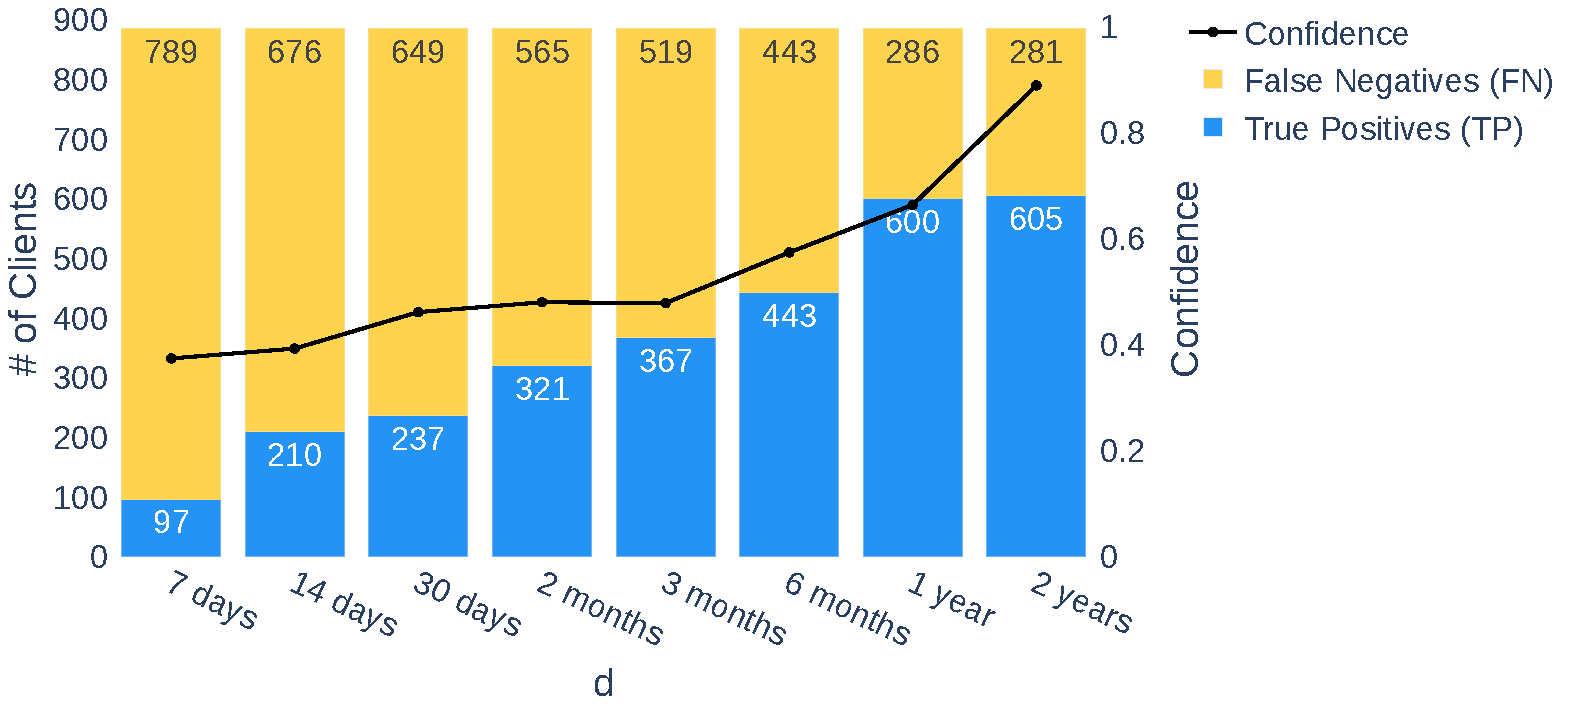
\includegraphics[width=1\textwidth]{Figures/Lazy-Columns.pdf}
% 		\caption{Confidence values taken from rule sets with Minimum Lift of 6.4.}
%     \label{fig:lazycol}
% \end{figure}

\subsection{Logistic Regression}
The Logistic Regression was integrated into the \Abb system by swapping out the Weighted Covering Algorithm rule set learner for Logistic Regression. This meant that five Logistic Regression models were trained (for five different values of $d$) and tested. 
Logistic Regression does not generate a model that can easily be saved and compared (like in rule set learning). The results presented in Section \ref{chap:results:rugresults} depend on having five trained models which were selected from a set of 10 trained by 10-fold stratified cross-validation. That is not possible with Linear Regression so instead, a simple 50-50 train/test split was performed. The model was trained on one split but evaluated on the entire dataset. This was done to ensure the numbers would line up with the other models.

% \begin{figure}[ht]
%     \centering
%     \figuretitle{Confidences using Logistic Regression}
%     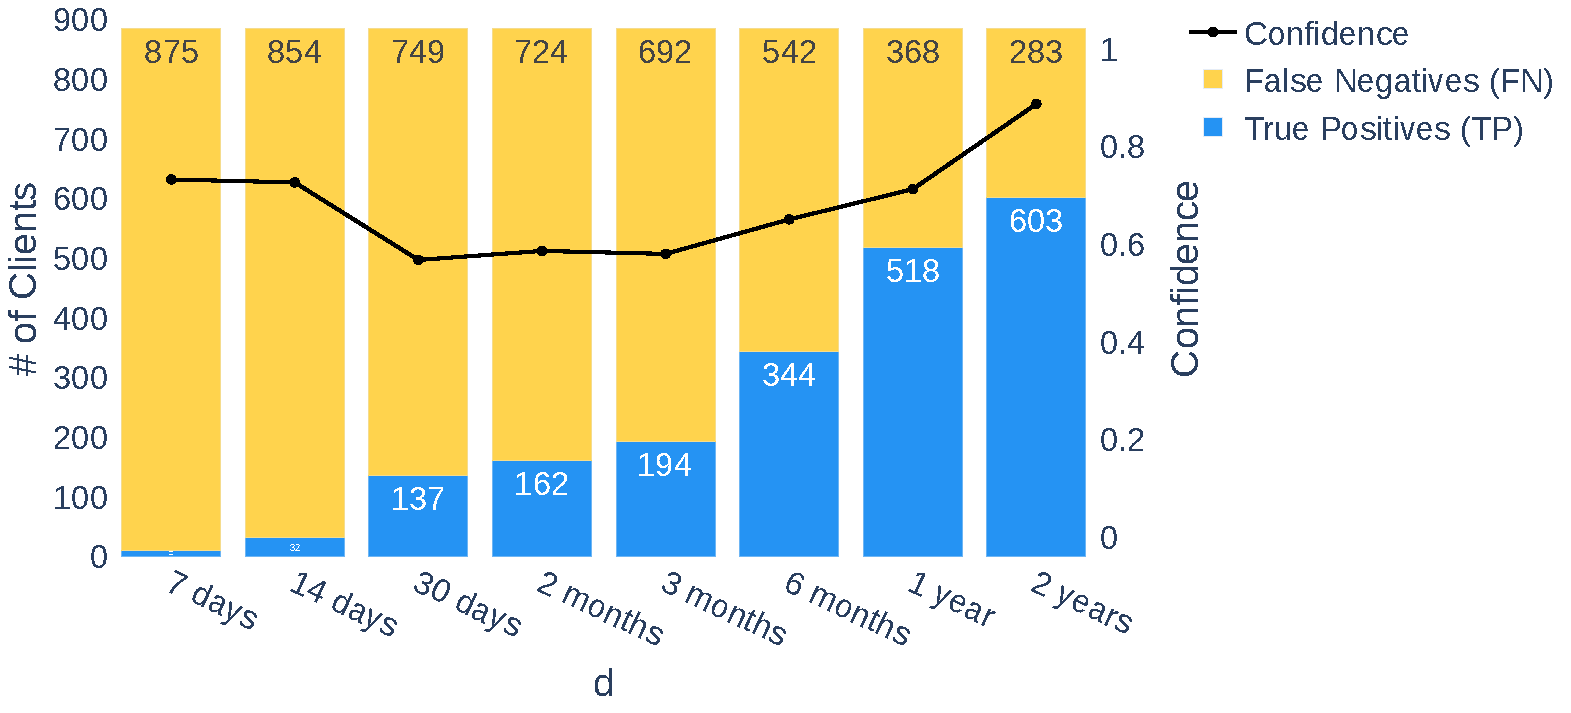
\includegraphics[width=1\textwidth]{Figures/LR-Columns.pdf}
% 		\caption{Confidence values taken from using Logistic Regression instead of rule set learning.}
%     \label{fig:lrcol}
% \end{figure}

\subsection{Results} \label{chap:results:rugresults}

Table \ref{tbl:results:abb} presents the results of the Greedy/Lazy systems and the Logistic Regression system.
In these results, the confusion values are presented without overlap between rule sets. What that means is that clients who are identified by one rule set (e.g. $d=7$) will be removed from the data set. This allows the Final row to be presented without over-inflating the number of individuals identified by the system. It also demonstrates the degree to which the generated rule sets do overlap. To display this removal, Table \ref{tbl:results:abb} has a new column, $N$, which is the cumulative sum of correctly identified individuals.

The Greedy system performs comparably to the single rule set with a Minimum Lift of 6.4 (Table \ref{tbl:results:30}). The benefit of the Greedy system can be seen by observing the distribution of the True Positive values with respect to the time scales. That is, the majority of clients (more than 100) are identified in fewer than 30 days (an average of around 29 days), with most of the rest being identified after 61 days. This is due to the overlap between the rule sets with short time scales, and rule sets with larger time scales. The rule sets with shorter time scales identify chronic clients early on, and those clients are then removed from the data set used by the rule sets with larger time scales, resulting in less identified clients. This is demonstrated in Table \ref{tbl:results:greedysets} where it can be seen that the rule sets generated at different time scales are similar. This is an example of the transparency that makes rule set based classifiers useful.

The Lazy system does not suffer the Sensitivity fall off quite as sharply as the Greedy system. This means that only about a third of identified clients are identified in less than 30 days (clients are identified after an average of around 33 days), and the rest are identified at a later time scale. There are about twice as many True Positives identified by the Lazy system, and this comes at the cost of having a little more than twice as many False Positives. The Lazy system also demonstrates the overlap, particularly at $d=14$ and $d=91$ where the Sensitivity is very low.

Comparing the results of the Lazy system with Table \ref{tbl:results:30}, it can be seen that the Lazy system performs somewhere between the single rule sets with Minimum Lift values of 2.5 and 6.4. The results of the Lazy system however have a more favourable Confidence/Sensitivity trade-off, with Confidence and Sensitivity being near the higher end of either single rule set scenario. Same as with the Greedy system, the real benefit of the Lazy system is that many of the clients are identified in two weeks or less.

The Logistic Regression system performs quite similar to the single time scale results presented in Table \ref{tbl:results:30}. The Confidence is approximately the same but the Sensitivity has improved by approximately 50\%. This Sensitivity increase comes from the redundancy of having five rule sets. Notably, the Linear Regression based system does not appear experience the Sensitivity falloff quite as sharply as the other two systems. The clients are identified at more even intervals, with a mean around 46 days. This appears to happen for two reasons. The first being that the Linear Regression system has a much lower Sensitivity at $d=7$ days, meaning that the overlap will be less pronounced as it is spread out more. The second is that the Linear Regression system is possibly training models that have less overlap than the rule set based systems. 

Overall there is no superior system based on Table \ref{tbl:results:abb}. All systems present a new set of Confidence/Sensitivity trade-offs and can situationally fit a user's needs depending on what those needs currently are. While it seems that both systems improved the rapid identification situation when compared to the single rule sets in Table \ref{tbl:results:30}, it is not exactly clear. In the following section, the MTTI metric will be used to compare the rapidity of identification.

\begin{table}[h]
	\centering

	\begin{tabular}{lrrrrrrrr}
	\toprule
	{$d$} &    $N$ &   TP &   FP &     TN &   FN &  Confidence &  Sensitivity &  Specificity \\
	\midrule
	\toprule
	Greedy & & & & & & & & \\
	\midrule
	7     &   95 &   95 &  150 &  17362 &  791 &    0.387755 &     0.107223 &     0.991434 \\
	14    &  109 &   14 &   16 &  17346 &  777 &    0.466667 &     0.017699 &     0.999078 \\
	30    &  115 &    6 &   11 &  17335 &  771 &    0.352941 &     0.007722 &     0.999366 \\
	61    &  183 &   68 &   42 &  17293 &  703 &    0.618182 &     0.088197 &     0.997577 \\
	91    &  186 &    3 &    9 &  17284 &  700 &    0.250000 &     0.004267 &     0.999480 \\
	Final &  186 &  186 &  228 &  17284 &  700 &    0.449275 &     0.209932 &     0.986980 \\
	\bottomrule
	\toprule
	Lazy & & & & & & & & \\
	\midrule
	7     &   95 &   95 &  150 &  17362 &  791 &    0.387755 &     0.107223 &     0.991434 \\
	14    &  109 &   14 &   16 &  17346 &  777 &    0.466667 &     0.017699 &     0.999078 \\
	30    &  264 &  155 &  195 &  17151 &  622 &    0.442857 &     0.199485 &     0.988758 \\
	61    &  366 &  102 &  157 &  16994 &  520 &    0.393822 &     0.163987 &     0.990846 \\
	91    &  373 &    7 &   21 &  16973 &  513 &    0.250000 &     0.013462 &     0.998764 \\
	Final &  373 &  373 &  539 &  16973 &  513 &    0.408991 &     0.420993 &     0.969221 \\
	\bottomrule
	\toprule
	Logistic Regression & & & & & & & & \\
	\midrule
	7     &   20 &   20 &    9 &  17503 &  866 &    0.689655 &     0.022573 &     0.999486 \\
	14    &   35 &   15 &    3 &  17500 &  851 &    0.833333 &     0.017321 &     0.999829 \\
	30    &  115 &   80 &   56 &  17444 &  771 &    0.588235 &     0.094007 &     0.996800 \\
	61    &  173 &   58 &   50 &  17394 &  713 &    0.537037 &     0.075227 &     0.997134 \\
	91    &  208 &   35 &   36 &  17358 &  678 &    0.492958 &     0.049088 &     0.997930 \\
	Final &  208 &  208 &  154 &  17358 &  678 &    0.574586 &     0.234763 &     0.991206 \\
	\bottomrule
	\end{tabular}

	\caption{Performance of the \Abb systems.}
	\label{tbl:results:abb}
\end{table}


\subsection{Mean Time To Identification}

The MTTI is a tool introduced in Chapter \ref{chap:algo} for comparing the rapidity of identification. This tool has been used with the Greedy, Lazy, and Logistic Regression systems.


The MTTI provides the mean time for all chronic clients to be identified as such. This means that clients that are not identified as chronic by the \Abb systems will still need to be identified by the DI definition. This results in MTTI values with a large number of days. To demonstrate how these systems compare on the clients they are able to identify, two new metrics are presented. The first is AIT, or Average Identification Time, which is the average time to identification for chronic clients who are identified by a system. The other is the Median Identification Time, which takes the median time to identification, rather than average. Total number of identified clients $N$ will be presented as well.

Table \ref{tbl:results:mtti} presents the MTTI values for the Greedy/Lazy systems, the Logistic Regression system, a system that uses a single rule set trained on 30 days (with a Minimum Threshold of 6.4), and using just the DI definition to classify individuals.
As stated in Section \ref{chap:algo:mtti}, the MTTI is the Mean Time to Identification for the 886 chronic clients in the data set. When a client is not identified by any of the classifier systems, the remaining unclassified individuals are assumed to be identified by the DI chronic definition after 666 days. The result of this is that all MTTI values are perhaps unexpectedly large. When evaluating a system based on MTTI, it is important to observe how many days less the MTTI value is when compared against the DI definition. The AIT and MIT values cover only the correctly identified future chronic individuals, they give a reference to how rapidly each system successfully identifies clients.
The Greedy system performs the worst of the four classifiers tested with the Logistic Regression system performing very similarly. The Lazy system performs the best, and the single time scale classifier performs somewhere in between. Looking back at Tables \ref{tbl:results:abb} and \ref{tbl:results:30} it appears that the reason for this relates with the Sensitivity of each system, having values of 0.21, 0.42, 0.23, and 0.27 respectively.
Another aspect of the Logistic Regression system that increased the MTTI value is the distribution of Sensitivity as seen in Table \ref{tbl:results:abb}. Logistic Regression has a fairly even distribution of Sensitivity compared to the Greedy and Lazy systems which would can be seen to increase the AIT by 15 days. 
This result suggests that the best way to identify individuals rapidly is to widen the net and allow many individuals to be identified at the cost of Confidence.
This result may also seem to suggest that the Greedy and Logistic Regression systems have poor performance, however, they require half the amount of housing resources as the Lazy system and still reduce the MTTI by over 100 days when compared to the DI definition alone. This could be a very useful heuristic for homeless shelters to use when housing resources are limited.


\begin{table}[h]
	\centering

	\begin{tabular}{lrrrr}
	\toprule
	{System} &  MTTI (days) & AIT (days) & MIT (days) & $N$ \\
	\midrule
	Greedy & 532 & 29.4 & 7 & 186 \\
	Lazy & 400 & 33.2 & 30 & 373 \\
	Logistic Regression & 520 & 45.5 & 30 & 208 \\
	$d=30$ & 496 & 30 & 30 & 237 \\
	DI Definition & 666 & 666 & 349 & 886 \\

	\bottomrule
	\end{tabular}

	\caption{The calculated MTTI values.}
	\label{tbl:results:mtti}
\end{table}

% \section{Demographics} \label{chap:results:demographics}
% \tdo{Discuss the need for looking at demographics}
% - definitions take a single slice of demographics, this can be more accurate
% \tdo{Display the demographic analysis results}

% \begin{table}[h]
% 	\centering

% 	\begin{tabular}{llll}
% 	\toprule
% 	{} &       min &      max &   median \\
% 	\midrule
% 	Age                          &        19 &       85 &       58 \\
% 	Bar (Count)                  &         0 &       55 &        0 \\
% 	CounsellorsNotes (Count)     &         0 &      443 &        7 \\
% 	EmployeeIsCounsellor (Count) &         0 &      464 &       11 \\
% 	EmsLogFlag (Count)           &         0 &       24 &        0 \\
% 	Log (Count)                  &         0 &     2419 &        8 \\
% 	PoliceLogFlag (Count)        &         0 &        8 &        0 \\
% 	ProgressDetails (Count)      &         0 &      539 &       13 \\
% 	Sleep (Count)                &         7 &     3380 &    243.5 \\
% 	Interactions (Count)         &         7 &     4517 &    354.5 \\
% 	Tenure (Days)                &         7 &     3733 &    696.5 \\
% 	Usage (\%)                    &  0.460678 &      100 &  78.2731 \\
% 	Average Gap Length (Days)    &  0.991935 &  233.692 &   1.2782 \\
% 	Stays (Count)                &         7 &     3380 &    243.5 \\
% 	Episodes (Count)             &         1 &       21 &        2 \\
% 	\bottomrule
% 	\end{tabular}

% 	\caption{}
% 	\label{tbl:results:demo}
% \end{table}



\section{Summary}

This chapter demonstrated the results of the \Abb system and compared those results against some more commonly used classification systems. These results demonstrated that the \Abb rule set learning system performs comparably to the standard interpretable classifiers. Additionally, the \Abb rule set learning is easily configurable to adjust the balance between Confidence and Sensitivity.

The MTTI metric was used to compare the Greedy/Lazy \Abb systems with a Logistic Regression based \Abb system. This demonstrated that Sensitivity is the most important metric when it comes to rapid identifications, but low Sensitivity classifiers can still be beneficial.

Overall the \Abb systems perform comparably to other classification systems but with an easy-to-understand set of steps and a clear/interpretable resulting model (rule sets). 
 \chapter{Conclusion} \label{chap:conclusion}

\section{Summary}

Classification rule learning is an interesting ML technique that can allow for fully interpretable output. The system proposed in this work (Chapter \ref{chap:algo}) takes this a step further by ensuring that each section of the process, Feature Generation, Single Rule Learning and Rule Set Learning strike a good balance between simplicity and performance. Specifically, this work uses a custom Feature Generation stage (Section \ref{chap:algo:binning}) that reduces the number of features without losing coverage of all attributes. A Single Rule Learning stage was also proposed (Section \ref{chap:algo:whypriori}) that utilizes the Apriori algorithm adapted for rule learning, which is essentially an exhaustive search over the space of all features. The Rule Set Learning stage (Section \ref{chap:algo:weightcov}) uses the Weighted Covering Algorithm, which is a slight departure from simplicity but allows for rules that overlap, allowing for a more intuitive rule set. 

The proposed \Abb system adds a layer on top of the classification rule learner that enables homeless shelters to identify clients within a much shorter time scale and still identify clients who do not exhibit chronic behaviours until after a much longer period. This work was evaluated with the proposed MTTI metric (Chapter \ref{chap:results}) and was able to outperform a single rule set as well as the DI definition.


Overall, this system shows promise and demonstrates the potential for use not just within homeless shelters, but any space where non-technical users need insight into machine learning models.


\section{Suggestions for Future Work}

As with all projects of this nature, there are several interesting extensions to this work that the author feels are worth pursuing. They are listed below in no specific order.

% The rule set learner in this work was the Apriori algorithm with the Weighted Covering algorithm. As mentioned in Chapter \ref{chap:algo}, this stage can be replaced by any other ML algorithm, based on the preference of the user. Notably, Chapter \ref{chap:results} demonstrated that the Logistic Regression algorithm would be a suitable and maybe even preferred replacement,

Chapter \ref{chap:results} demonstrated two hypothetical heuristics for setting the Minimum Lift Threshold. Rather than depending on a heuristic a higher level covering algorithm could be employed that would iteratively generate rule sets (as opposed to the standard covering algorithm that generates rules) and optimize for some user-supplied value.

As noted in Chapter \ref{chap:algo} this work makes predictions based on the $d$ days following a client's first sleep in shelter. This does not fit perfectly with real patterns of homelessness. A real client will not necessarily demonstrate patterns of chronic homelessness immediately upon their first stay in shelter. Client's will often experience multiple episodes of homelessness before becoming chronic. For example, a client might not demonstrate patterns of chronic homelessness the first time they sleep at the DI, but they may return after a few years and show chronic patterns at that time. A future system should take this into account and consider a client's $d$ days since first sleep, as well as the first $d$ days of the current episode.

The final suggestion departs from the typical supervised learning model used in this work. The chronic definition employed at shelter and government levels is a rough measure for homelessness that only considered sleeps (and sometimes episodes). Thus any bias from this non-perfect measure will be present in an ML system trained with chronic labels generated from the standard measures. This is similar to the selectively labelled data problem highlighted by Lakkaraju et al. \cite{lakkaraju2017selective}, however in this case the bias is introduced by a human-made measure.
The author proposes to instead use a new rule quality metric Stays Saved \cite{messier2020} which will consider the total stays of each client, as well as the number of stays the client has experienced at the theoretical time of learning. That is, for a rule set being generated with $d=7$, a client's number of stays is guaranteed to be less than 7 but the total number of stays can be much greater. The Stays Saved metric will calculate the difference between these values for each client and sum them. This single metric can then be used to evaluate and compare rules. A rule set generated using Stays Saved as a training metric will be more closely aligned with the actual purpose of identifying chronic individuals, that is, minimizing the total time that homeless individuals spend in shelter. 


%%%%%%%%%%%%%%%%%%%%%%%%%%%%%%%%%%%%%%%%%%%%%%%%%%%%%%%%%%%%%%%%%%%%%%%%
%                                                                     %%
% Bibliography                                                        %%
%                                                                     %%
%%%%%%%%%%%%%%%%%%%%%%%%%%%%%%%%%%%%%%%%%%%%%%%%%%%%%%%%%%%%%%%%%%%%%%%%

%% As required by the 2014 thesis guidelines, the bibliography must
%% appear in the table of contents. Do not remove the following lines. 
  \cleardoublepage\phantomsection
  \addcontentsline{toc}{chapter}{Bibliography}
  
%% There are multiple options for assembling a bibliography in LaTeX.
%% Some of these options include:

%%%%%%%%%%%%%%%%%%%%%%%%%%%%%%%%%
%%  BiBTeX
\bibliographystyle{ieeetr}
\bibliography{BiblThesis}

%%%%%%%%%%%%%%%%%%%%%%%%%%%%%%%%%%%%%%%%%%%%%%%%%%%%%%%%%%%%%%%%%%%%%%%%
%%                                                                    %%
%% Appendices                                                        %%
%%                                                                    %%
%%%%%%%%%%%%%%%%%%%%%%%%%%%%%%%%%%%%%%%%%%%%%%%%%%%%%%%%%%%%%%%%%%%%%%%%

  \appendix             %% Do not remove this line

	\chapter{Measuring Performance} \label{chap:perf}

% \tdo{Re-read this}
% \tdo{Maybe expand on the Accuracy and why it is bad}

% \begin{epiquote} 
%  \textit{When a measure becomes a target, it ceases to be a good measure.}
% \end{epiquote}    
% \begin{flushright} - \textit{Goodhart's Law}\end{flushright}\bigskip

 It is important to understand the benefits and downsides of using a specific measure when training a machine learning system. In this Appendix, a framework for theoretical rule analysis \cite{furnkranz2005roc} will be presented (Section \ref{chap:perf:background}). This framework will then be used to compare several common performance measures (Section \ref{chap:perf:measures}). Consideration will be made for the specific challenges presented by this work (i.e. the imbalance between the number of chronic and not chronic clients), however, this appendix will not be using data from the DI, and will instead focus on the theoretical use of the presented measures. 


\section{Background} \label{chap:perf:background}

% 35 if my counting is correct
There are over 30 measures for comparing binary classification systems in Foundations of Rule Learning \cite{furnkranz2012foundations}. However, each measure presents a specific trade-off between reinforcing true positives and penalizing false positives (or reinforcing true negatives and penalizing false negatives). Understanding this trade-off is of utmost importance when selecting a measure as it directly translates to the usefulness of the generated model.

This work is performed within the context, of housing operations where, due to budget and housing constraints, it is infeasible to house every client. In the standard classification context it is generally considered equal to increase the covered true positives or to decrease the covered false positives. However, in this context, adding additional covered clients can mean exceeding the capacity of a housing program. With this work, there will be a preference for decreasing the covered false positives when given the opportunity. Unfortunately, this trade-off is often unclear when looking at a measure definition, ideally, there would be a way to visualize this trade-off for each measure.

Receiver Operating Characteristic (ROC) \cite{Fawcett2006AnIT} analysis is a popular method of visualizing classifier performance. While the most common usage is the ROC curve, ROC analysis can take other forms. F{\"u}rnkranz and Flach \cite{furnkranz2005roc} demonstrate a method of using the ROC space to visualize the inherent true positive/false positive trade-off presented by different measures.

In this appendix, a modification of ROC space, called coverage space \cite{furnkranz2005roc}, will be used to visualize the differences between the measures. Coverage space only differs from ROC space in that it plots the number of true positives vs. false positives, rather than the true positive rate and false positives rate typically used in ROC space. 
In most cases, the plots will be almost identical between coverage space and ROC space, but coverage space tends to more accurately represent a measure by using the non-normalized values. This is particularly helpful when analyzing rules in the context of a skewed data set.

The rest of this appendix will adopt the notation used in Foundations of Rule Learning \cite{furnkranz2012foundations}. Within this appendix, these are purely theoretical values and not the result of having run any form of classifier. However, later appendix will adopt the same notation when presenting classification results.


\begin{align*}
	\mathcal{E} &= \text{Set of all examples (set of all clients)} \\
	\mathcal{P} &= \text{Set of positive examples} \\
	\mathcal{N} &= \text{Set of negative examples} \\
	P &= \text{Number of positive examples} = \hat P + \bar P = |\mathcal{P}| \\
	N &= \text{Number of negative examples} = \bar N + \hat N |\mathcal{P}| \\
	\hat P &= \text{Number of correct positive classifications (True positives)} \\
	\hat N &= \text{Number of incorrect positive classifications (False positives)} \\
	\bar P &= \text{Number of incorrect negative classifications (False negatives)} \\
	\bar N &= \text{Number of correct negative classifications (True negatives)} \\
\end{align*}


In this appendix only the set sizes will be used ($P, N, \hat P, \hat N, \bar P, \bar N$). Within figures, TP and FP will be used instead of $\hat P$ and $\hat N$ respectively.

Table \ref{tbl:perf:examples} presents two example classifications. These classifications are completely fabricated and are only represented by the confusion values. These examples will be used in the following section to compare the performance of different measures. These examples are created from a sample of 200 individual classifications. The Random example is an example of a randomized classifier, i.e. the classifier used predicts True 70\% of the time no matter what. The Good example is completely fabricated and demonstrates a pretty good classification. More examples will be introduced in the next section as needed.

\begin{table}[h]
	\centering

	\begin{tabular}{lrrrr}
	\toprule
	{} &    $\hat P$ & $\hat N$ & $\bar N$ & $\bar P$ \\
	\midrule
	Random & 70 & 70 & 30 & 30 \\
	Good   & 98 & 16 & 84 & 2  \\
	\bottomrule
	\end{tabular}

	\caption{Example classifications.}
	\label{tbl:perf:examples}
\end{table}


\section{Measures} \label{chap:perf:measures}

In this section, the three measures from association rule learning (Support, Confidence, and Lift) will be presented along with the Relative Linear Cost (RelLinCost) measure and the Accuracy measure.
The justification for selecting these measures is due to their popularity within the fields of association rule learning, classification rule learning, and machine/deep learning respectively.
The analysis taken in this section follows the one done by F{\"u}rnkranz and Flach, 2005 \cite{furnkranz2005roc} \cite{furnkranz2012foundations}, with a focus on the above rules.


First, a brief introduction into using coverage space as a tool for comparing measures. In typical usage of ROC space, the results of a single classification will be plotted ($\hat P$ and $\hat N$) as a point, and multiple classifications can be plotted by tweaking a threshold or a parameter in the classifier. When multiple classifications are plotted it will form a curve through the ROC space, called an ROC curve.

Points in the upper left corner of the plot $(0, P)$ (or lines that cross this point) are ideal because the corner represents a perfect prediction. Points in the bottom right are also good because the model can be inverted to obtain perfect predictions. Any point lying along the line $\hat P = \hat N$ is considered to be equivalent to a random guess because the probability of a true positive is equal to the probability of a false positive ($\text{P}(\hat P) = \text{P}(\hat N)$). A good measure will assign any point along this line a low score, and assign the maximum score to the point $(0, P)$. In the case where $P = N$, this line has a slope of 1, however, when used in the presence of class imbalance ($P \neq N$), the slope will be $P/N$. Because of the slope change, the line will always stretch from the bottom left corner to the top right corner of the coverage space. 

F{\"u}rnkranz and Flach's use of the coverage space does not depend on having classification results. They instead produce a 3D plot of a measure evaluation over the entire range of $\hat P$ and $\hat N$. This measure evaluation is a surface in 3D space. The gradient of this plot gives insight into the trade-off between true positives and false negatives. This 3D plot is represented in two dimensions using just the isometrics. An isometric is a line that represents all measures of the same value. Looking at a plot of isometrics is the same as looking at a 2D height map, the gradient can be observed as being perpendicular to the isometrics.
 
To demonstrate this the MinFP (Minimum False Positive) measure is introduced
$MinFP(\hat P, \hat N) = 1-\frac{\hat N}{N}$
. The MinFP measure is a simple measure that tracks how small the value of $\hat N$ is for a classifier. That is, a classifier with a low value of $\hat N$ will have a high MinFP score.

Figure \ref{fig:minfp} demonstrates the resulting isometric plot, which shows that the isometrics are equally spaced vertical lines. Any point along these vertical lines has the same MinFP value. The intuition that comes from looking at this plot is that MinFP does not properly account for true positives. This is rather obvious from the definition, and in the case of MinFP, the isometric plot is not very informative but stands as an example of the format.

This can be seen further by comparing the Good classification and an example classification that has the same MinFP score. It is clear from Figure \ref{fig:minfp} that the Match example is worse than the Good example, yet will still have the same MinFP score.

\begin{figure}[ht]
    \centering
    \figuretitle{Min FP}
    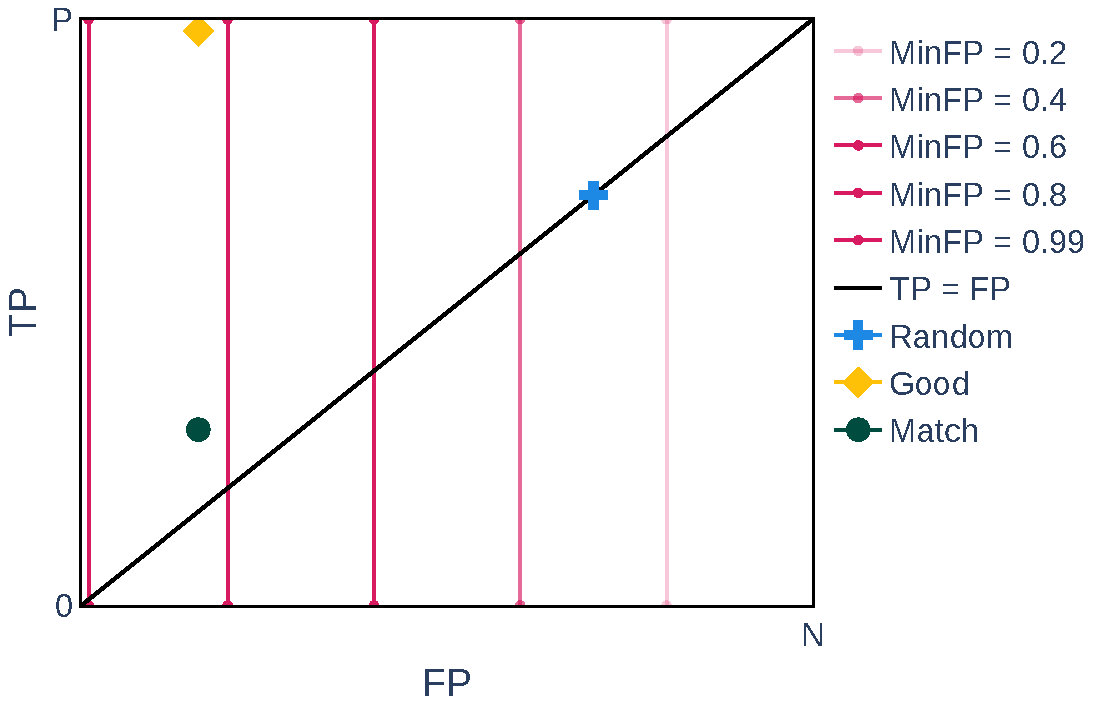
\includegraphics[width=0.7\textwidth]{Figures/MP-MinFP}
		\caption{Isometric plot for the MinFP measure.}
    \label{fig:minfp}
\end{figure}


\FloatBarrier
\subsection{Accuracy}

Accuracy is perhaps the most well-known measure, if only due to its familiar name. The reason for this popularity is clear when looking at the isometrics (Figure \ref{fig:accuracy}), which are parallel to the center line and evenly step towards the top left corner of the coverage space plot. This aligns exactly with the intuition one would develop from looking at the ROC/coverage space. The definition of Accuracy:
$Accuracy(\hat P, \hat N) = \frac{\hat P + \bar N}{P + N}$
demonstrates the reason for these isometrics, namely that Accuracy considers both true positives and true negatives in equal proportion, scaled by the total number of samples.

Intuitively, Accuracy is the proportion of correct classifications. An Accuracy of 1.0 (100\%) is thus the optimal metric, and a score of 0.5 (50\%) corresponds to a random guess. This is a good heuristic when $P \approx N$, however, it falls apart when $P$ and $N$ diverge. Figure \ref{fig:accuracy-bias} demonstrates such a case where $P = 0.2 N$, as can be seen, the isometrics skew towards the over-represented class and even relatively large changes in the minority class have little effect on the Accuracy score. This also corrupts the intuitive understanding of Accuracy as the $\hat P = 0.2 \hat N$ line is no longer aligned with an Accuracy score of 0.5. 

Figures \ref{fig:accuracy} and \ref{fig:accuracy-bias} use an additional example also called Match with values of 0.84, 0.02, 0.98, and 0.16 for $\hat P$, $\hat N$, $\bar N$, and $\bar P$ respectively. In the balanced class case $P=N$, the Random classifier has an Accuracy of 0.5, while the Good and Match classifiers have an Accuracy of 0.91. In the case with class imbalance ($P = 0.2 N$), the Random classifier now has an Accuracy of 0.7, the Good classifier has an Accuracy of 0.86, and the Match classifier has an Accuracy of 0.96.

This behaviour is undesirable for two reasons. The first is that the relative ordering of the Good and Match examples has changed when the underlying class distribution changed. This means that any classifier that uses Accuracy during the training phase will be extremely sensitive to the class distribution of the underlying data. For example, a classifier might be trained on a data set with a class distribution of X, and an Accuracy of 0.96. This classifier can then be employed on a new data set with class distribution Y, and an Accuracy of 0.8, even though the performance in terms of $\hat P$ and $\hat N$ might be identical. The second reason is that users of this system will not be able to build a proper intuition around what Accuracy means. Looking at the Random example, the Accuracy in the imbalanced case (0.7) appears good but still corresponds to a random guess.

 % Transparency is key in this work meaning that the lack of intuitive interpretation for Accuracy when working with the DI data ($P \approx 0.04 N$) makes it unsuitable for use.

\begin{figure}[ht]
    \centering
    \figuretitle{Accuracy}
    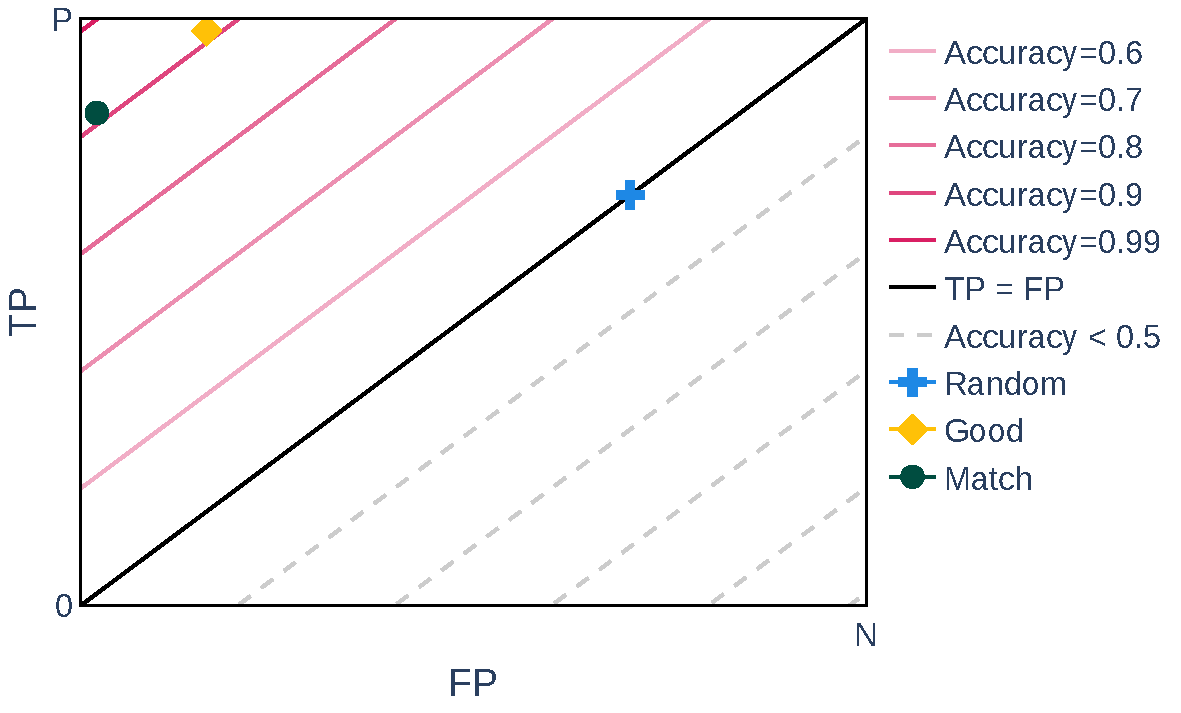
\includegraphics[width=0.7\textwidth]{Figures/MP-Accuracy}
		\caption{Isometric plot for the Accuracy measure.}
    \label{fig:accuracy}
\end{figure}
\begin{figure}[ht]
    \centering
    \figuretitle{Accuracy; P = 0.2 N}
    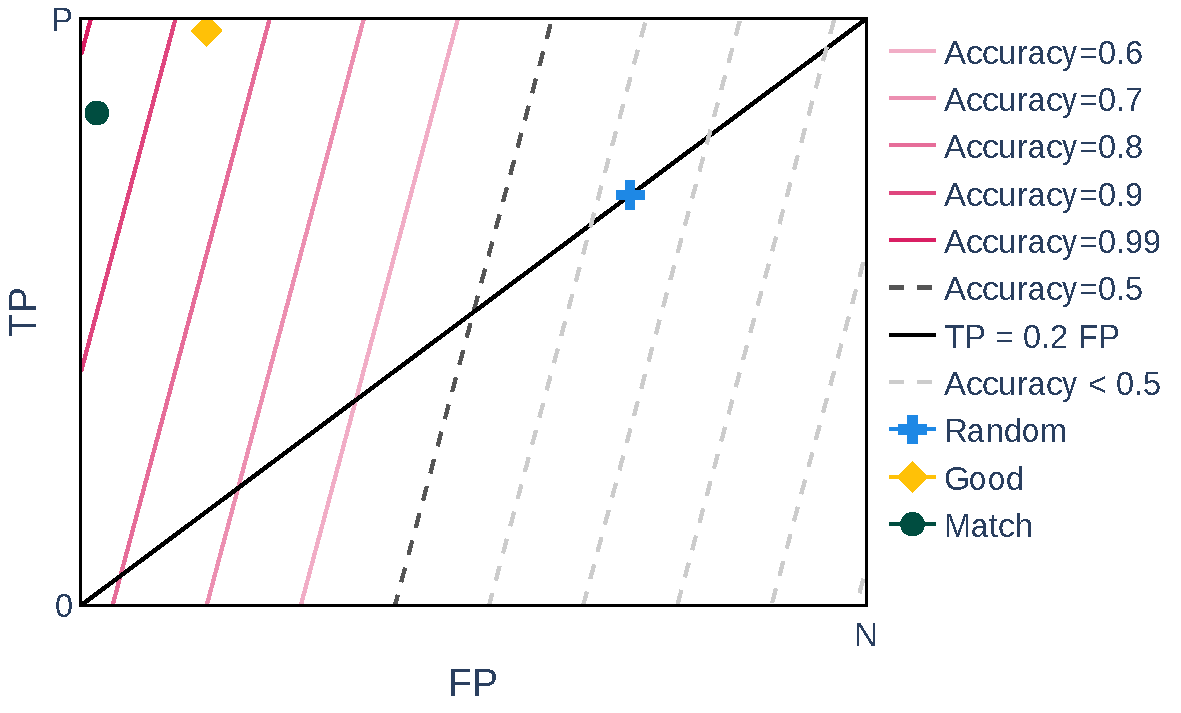
\includegraphics[width=0.7\textwidth]{Figures/MP-Accuracy-bias}
		\caption{Isometric plot for the Accuracy measure with a skewed class distribution.}
    \label{fig:accuracy-bias}
\end{figure}

\FloatBarrier
\subsection{Relative Linear Cost}

RelLinCost is a popular measure \cite{furnkranz2012foundations} within the field of classification rule learning. It is similar to Accuracy in that the isometrics perfectly sweep from the mid-line to the top-left corner (Figure \ref{fig:rellincost}). However, RelLinCost differs from Accuracy when working on an unbalanced data set. 
This is due to the configurable parameters $a$ and $b$ which can be seen in the definition of RelLinCost
$RelLinCost(\hat P, \hat N, a, b) = a  \frac{\hat P}{P} - b \frac{\hat N}{N}$
. This allows the system designer to configure a trade-off between true positives and false positives based on the specifics of the problem. A common use case is to have $a=1$ and $b=1$ which place equal importance on maximizing the true positive rate and minimizing the false positive rate. This presents a powerful tool in terms of designing a training system with configurable priorities.

RelLinCost can be seen as a generalization of Accuracy. Equation \ref{eq:rellincost-derive} demonstrates how the variables $a$ and $b$ can be configured to approximate Accuracy. This is only an approximation due to the dangling $\frac{N}{P+N}$, fortunately, this term will be constant and will not affect the relative ordering for model scores.

Because RelLinCost compares the rates rather than raw values, it will not suffer from the same issues as Accuracy when the underlying class distribution changes. Figure \ref{fig:rellincost-bias} demonstrates the case where $P = 0.2 N$. As can be seen in Figure \ref{fig:rellincost-bias} the isometrics of RelLinCost do not change when underlying class distribution changes (but can be adjusted using $a$ and $b$).

Additionally, the position of the three example points does not move when the class imbalance is introduced. This means that the intuition that users build up around what RelLinCost means will not change when the underlying class distribution changes. This makes RelLinCost an exceptionally robust measure.

\begin{equation} \label{eq:rellincost-derive}
    \begin{split}
    a = \frac{P}{P+N}; &\quad
    b = \frac{N}{P+N} \\
		RelLinCost(\hat P, \hat N, a, b) &= Accuracy(\hat P, \hat N) - \frac{N}{P+N}
    \end{split}
\end{equation}
\begin{figure}[ht]
    \centering
    \figuretitle{Relative Linear Cost}
    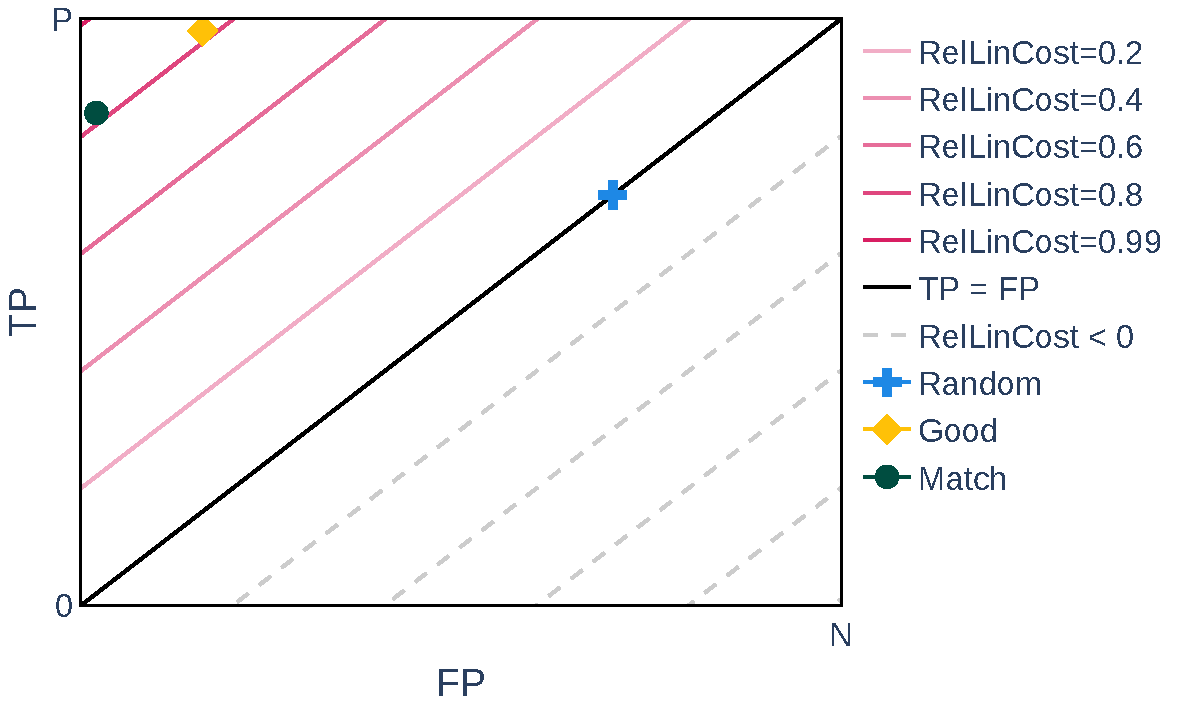
\includegraphics[width=0.7\textwidth]{Figures/MP-RelLinCost}
		\caption{Isometric plot for the RelLinCost measure.}
    \label{fig:rellincost}
\end{figure}
\begin{figure}[ht]
    \centering
    \figuretitle{Relative Linear Cost; P = 0.2 N}
    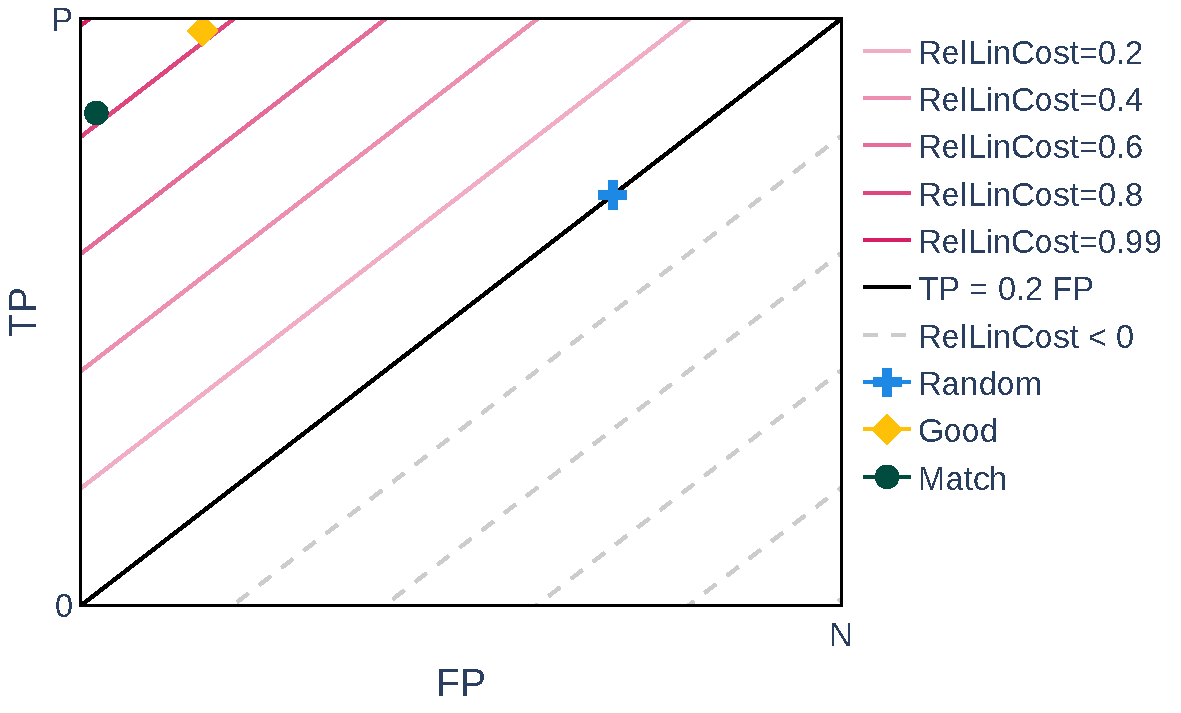
\includegraphics[width=0.7\textwidth]{Figures/MP-RelLinCost-bias}
		\caption{Isometric plot for the RelLinCost measure with a skewed class distribution.}
    \label{fig:rellincost-bias}
\end{figure}

\FloatBarrier
\subsection{Support}

Support is the most basic measure of model performance from the field of association rule learning. The definition of Support in terms of the confusion values is
$Support(\hat P, \hat N) = \frac{\hat P}{P+N}$
. An alternative definition for Support is $Support(\hat P, \hat N) = \text{P}(\hat P)$ i.e. Support is the observed probability of a true positive.
Figure \ref{fig:sup} demonstrates the isometrics of Support. These isometrics are directly perpendicular to that of MinFP, Support does not account for false positives and will thus tend towards the top-right of the coverage space when learning a rule. While Support alone is not sufficient for this work, it can be used in conjunction with another measure (commonly Confidence) to enforce a minimum number of acceptable true positives.

\begin{figure}[ht]
    \centering
    \figuretitle{Support}
    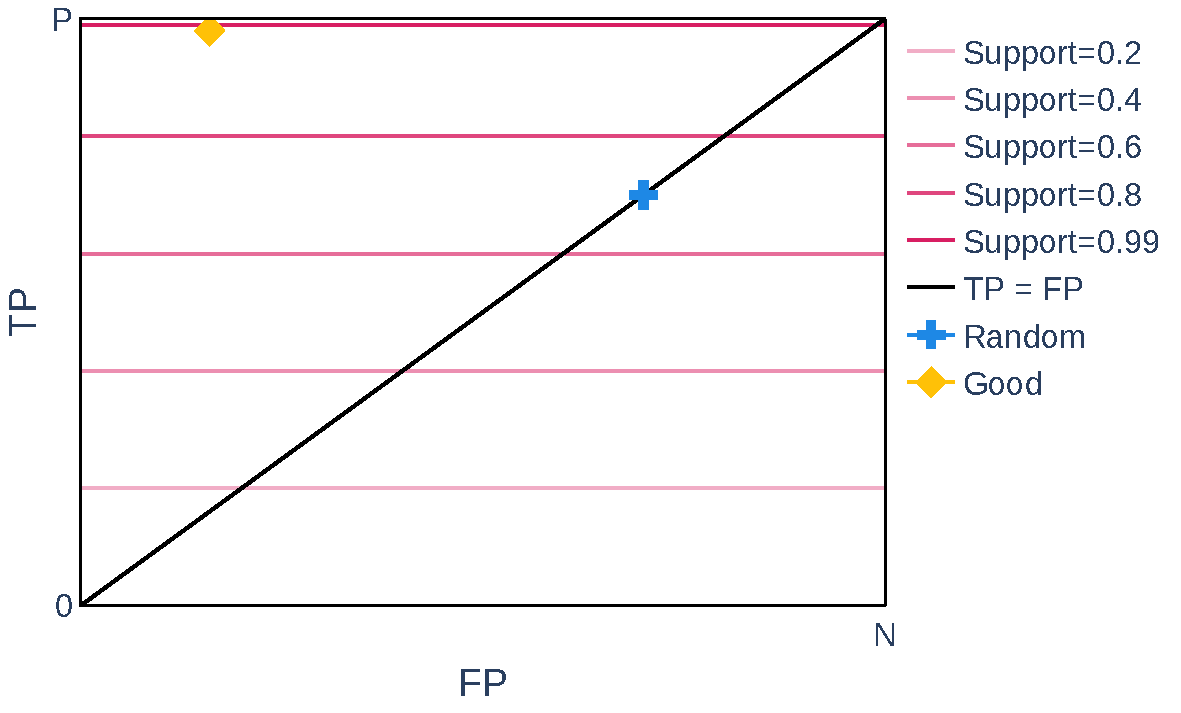
\includegraphics[width=0.7\textwidth]{Figures/MP-Support}
    \caption{Isometric plot for the Support measure.}
    \label{fig:sup}
\end{figure}

\FloatBarrier
\subsection{Confidence}

Confidence (also known as Precision) is another measure that comes out of the field of association rule learning. The definition of Confidence with respect to the confusion values is
$Confidence(\hat P, \hat N) = \frac{\hat P}{\hat P+\hat N}$
. Intuitively, Confidence is the proportion of correctly classified examples. This can also be stated as the conditional probability
\\$\text{P}(\text{Positive example}| \text{Positive classification})$. This intuition makes Confidence highly desirable when sharing results with a non-technical audience.

As can be seen in Figure \ref{fig:conf}, the Confidence measure does account for both $\hat P$ and $\hat N$. However, it only looks at the values in proportion to one another, meaning that a rule with 0 true positives can rate as high as one with $\hat P = P$. Fortunately, this can be compensated for by using the Support measure together with Confidence. Where the Support measure is used to provide a minimum threshold on the number of true positives and Confidence is used to rank models that pass that threshold. This is not always desirable, as it reduces the use of Confidence to be very similar to MinFP. However, in this work, it is preferable to minimize $\hat N$ over maximizing $\hat P$ and Confidence allows for a convenient trade-off while remaining intuitive. 

For Confidence a Match example with $\hat P$, $\hat N$, $\bar N$, and $\bar P$ of 0.3, 0.05, 0.95, 0.7 respectively are used. The Random example has a Confidence of 0.5, the Good and Match examples have a Confidence of 0.86. When the class imbalance is introduced (Figure \ref{fig:conf-bias}) the Random example Confidence becomes 0.167, the Good and Match Confidence becomes 0.55. This is better than the Accuracy example because the Good and Match examples still have the same Confidence. This means that Confidence is a suitable measure for use in the learning stage because learning algorithms (e.g. the Apriori algorithm) only rely on relative sorting of rules, which does not change in this case. However, the intuitive understanding of Confidence is no longer clear in the case of class imbalance, where a Random guess now has a Confidence of 0.167.


\begin{figure}[ht]
    \centering
    \figuretitle{Confidence}
    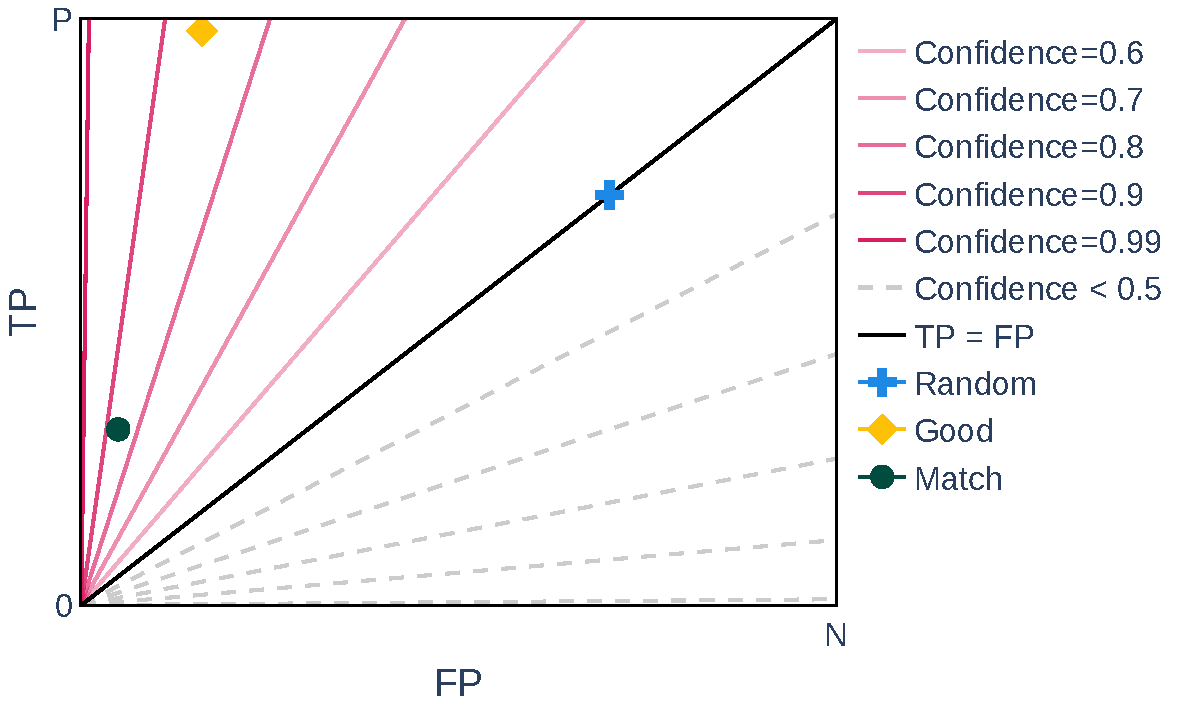
\includegraphics[width=0.7\textwidth]{Figures/MP-Confidence}
		\caption{Isometric plot for the Confidence measure.}
    \label{fig:conf}
\end{figure}
\begin{figure}[ht]
    \centering
    \figuretitle{Confidence; P = 0.2 N}
    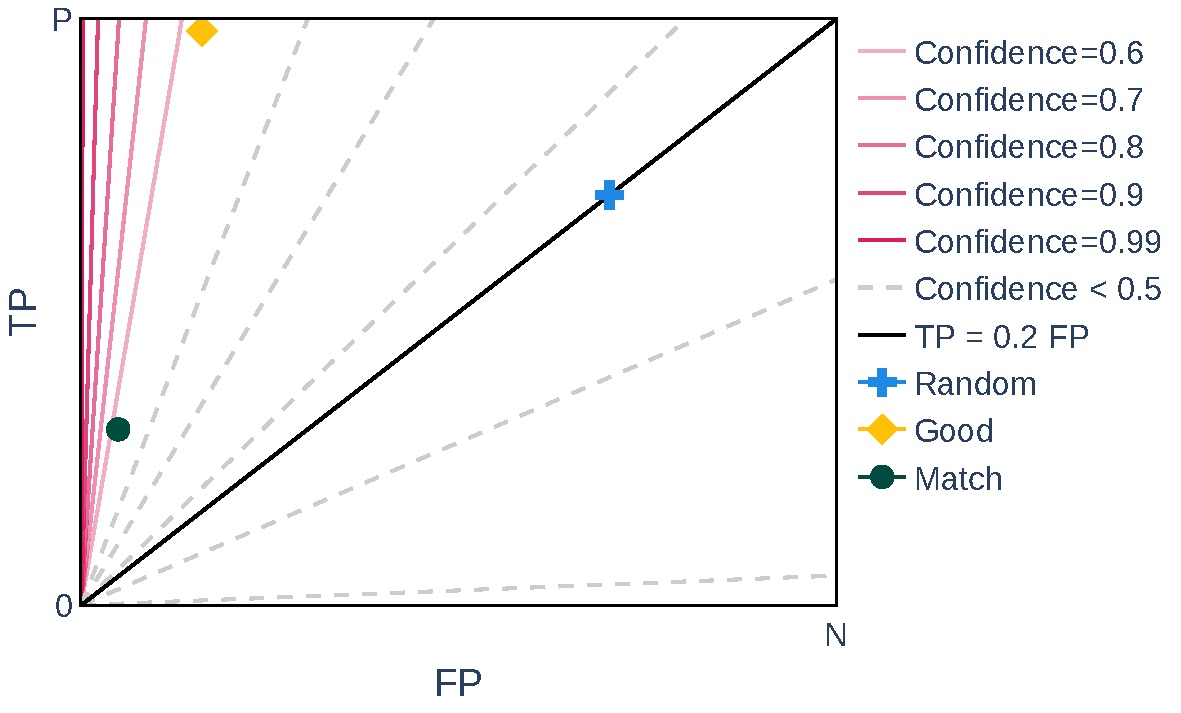
\includegraphics[width=0.7\textwidth]{Figures/MP-Confidence-bias}
		\caption{Isometric plot for the Confidence measure with a skewed class distribution.}
    \label{fig:conf-bias}
\end{figure}

\FloatBarrier
\subsection{Lift}

Lift is the final measure that comes from the field of association rule learning. The definition of Lift is
$Lift(\hat P, \hat N) = \frac{\frac{\hat P}{\hat P+\hat N}}{\frac{P}{P+ N}}$
. Intuitively, Lift is the relative performance increase (or decrease) of a classification model when compared to a random guess. In this context, a random guess is a random decision with a probability matching that of the underlying data, $\frac{P}{P+N}$ in this case. This makes judging the quality of a rule based on Lift trivially easy as and value $>1$ is by definition better than a random guess. 

Figure \ref{fig:lift} demonstrates the isometrics of Lift. As can be seen, these are identical to those of Confidence. This does not suggest that the two measures are the same, they clearly output different values, but when used to evaluate the relative performance of a machine learning model Confidence and Lift will always match.
Figure \ref{fig:lift-bias} shows the same figure under a new class distribution ($P = 0.2 N$). 
Here the Match example is the same as used with Confidence. Lift differs from Confidence because it is normalized by the underlying class distribution (similar to RelLinCost). This means that when class imbalance is introduced the values of Lift change, but the Lift value corresponding to a random guess (1) and the relative values between the Good and Match classifier do not change. This means that users do not lose the fundamental intuition that Lift $> 1$ is good, and the training system can still rely on the order of classifiers based on Lift.

Lift can also benefit from the use of Support described above. This gives Lift all the same benefits as Confidence in the context of model training, but benefits from a consistent, intuitive interpretation for any class distribution.

\begin{figure}[ht]
    \centering
    \figuretitle{Lift}
    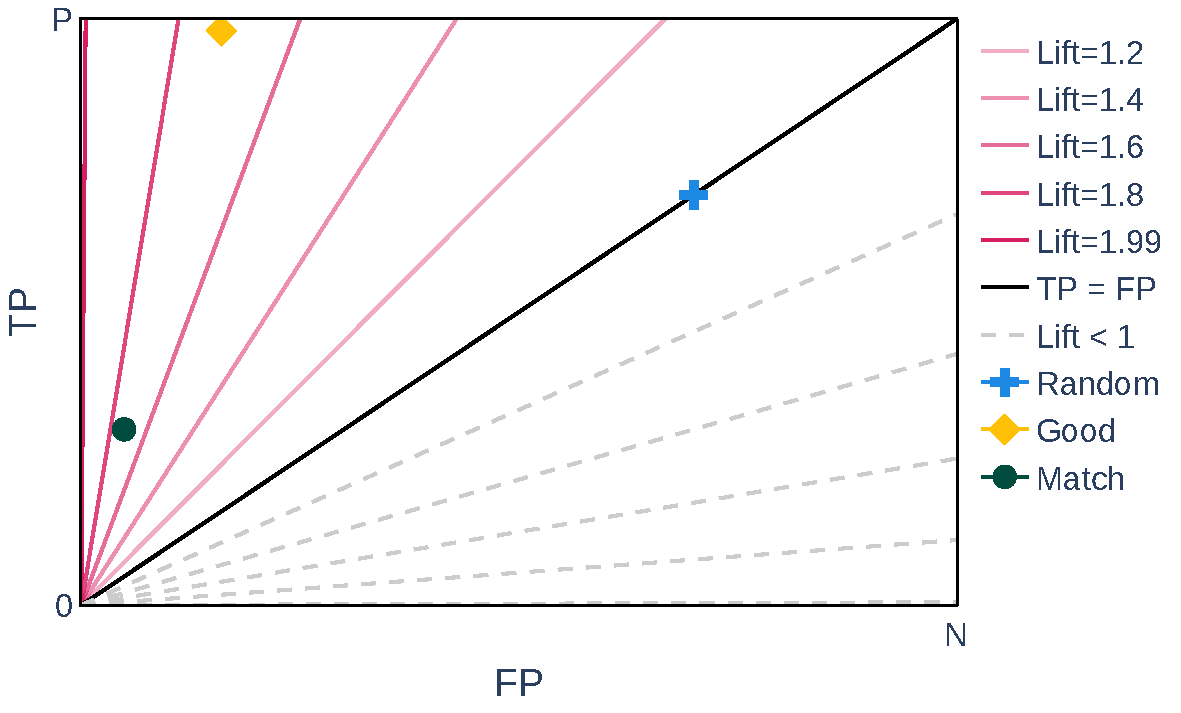
\includegraphics[width=0.7\textwidth]{Figures/MP-Lift}
		\caption{Isometric plot for the Lift measure.}
    \label{fig:lift}
\end{figure}
\begin{figure}[ht]
    \centering
    \figuretitle{Lift; P = 0.2 N}
    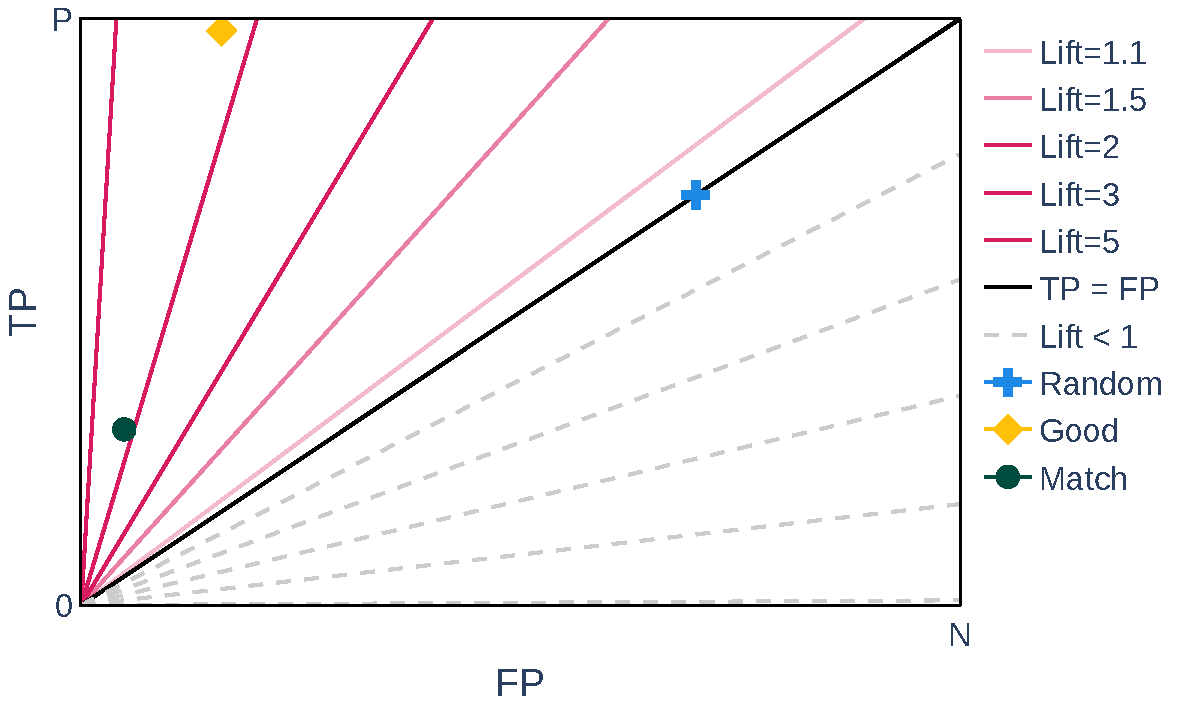
\includegraphics[width=0.7\textwidth]{Figures/MP-Lift-bias}
		\caption{Isometric plot for the Lift measure with a skewed class distribution.}
    \label{fig:lift-bias}
\end{figure}


\FloatBarrier
% \subsection{Decision}
% As transparency is a key focus of this work, it is important that the measure used for model training is the same as the measure presented to users. This prevents inconsistencies between the generated order of rules, and the order as seen by users. 

% Only RelLinCost and Lift have been identified as suitable for use in this work. Both perform well with varying class distributions and both present an intuitive understanding. For RelLinCost any values from 0-1 are improvements where 1 is the best and 0 is no improvement. For Lift any value above 1 is an improvement, the larger the better.
% Lift was selected for model training and presentation. The intuitive interpretation of Lift as "X times better than a random guess" is beneficial to users of the system who might not grasp RelLinCost and it fits with the training system introduced in chapter \ref{chap:algo}. 


\section{Conclusion}

The Accuracy, RelLinCost, Support, Confidence, and Lift measures were all discussed. It was found that Accuracy and Confidence lose their intuitive understanding when used with data sets that have a large degree of class imbalance. RelLinCost, Support, and Lift maintain the same understanding despite the change in underlying distribution. Support is lacking however in presenting the full picture of classification performance as it does not consider False Positives. RelLinCost and Lift are both suitable for use in this work, based on the above analysis. However, Lift will be the measure used in this work as it is already used by the Apriori algorithm and has a more consistent and intuitive representation than any of the other measures presented here.



%%%%%%%%%%%%%%%%%%%%%%%%%%%%%%%%%%%%%%%%%%%%%%%%%%%%%%%%%%%%%%%%%%%%%%%%
%%                                                                    %%
%% End of document                                                    %%
%%                                                                    %%
%%%%%%%%%%%%%%%%%%%%%%%%%%%%%%%%%%%%%%%%%%%%%%%%%%%%%%%%%%%%%%%%%%%%%%%%
\end{document}          %% Do not remove this line

%%
%% End of file `ucalgarythesis.tex'.
%%%%%%%%%%%%%%%%%%%%%%%%%%%%%%%%%%%%%%%%%%%%%%%%%%%%%%%%%%%%%%%%%%%%%%%

